\documentclass[11pt,a4paper]{article}

\usepackage[utf8]{inputenc}
\usepackage[T1]{fontenc}
\usepackage{babel}
\babelprovide[main,import]{spanish}
\usepackage{lmodern}
\usepackage[a4paper,margin=2.1cm,headheight=15pt]{geometry}
\usepackage{microtype,graphicx,longtable,booktabs,tabularx,array,xcolor,enumitem,hyperref,fancyhdr,caption,float,pdflscape,seqsplit,cite}
\usepackage[most]{tcolorbox}
\definecolor{Navy}{HTML}{17365D}
\definecolor{Teal}{HTML}{1F7A8C}
\definecolor{Light}{HTML}{EAF2F8}
\definecolor{Green}{HTML}{D9EAD3}
\definecolor{Amber}{HTML}{FFF2CC}
\hypersetup{colorlinks=true,linkcolor=Navy,urlcolor=Teal,citecolor=Navy,pdftitle={PE5 FabroGym - Integracion, metricas y defensa}}
\graphicspath{{../assets/}}
\pagestyle{fancy}\fancyhf{}\fancyhead[L]{\small PE5 - FabroGym}\fancyhead[R]{\small Equipo F (PE5) - 2026}\fancyfoot[C]{\thepage}
\setlength{\parindent}{0pt}\setlength{\parskip}{5pt}\setlist{nosep}
\renewcommand{\arraystretch}{1.15}
\newcolumntype{Y}{>{\raggedright\arraybackslash}X}
\newtcolorbox{reqbox}[2][]{enhanced,breakable,colback=white,colframe=Navy,title={#2},fonttitle=\bfseries,coltitle=white,boxrule=.7pt,arc=1mm,left=5pt,right=5pt,top=4pt,bottom=4pt,#1}
\newtcolorbox{alertbox}[1][]{enhanced,breakable,colback=Amber,colframe=Teal,boxrule=.7pt,arc=1mm,left=6pt,right=6pt,top=5pt,bottom=5pt,#1}
\captionsetup{font=small,labelfont=bf}

\begin{document}
\hypersetup{pageanchor=false}

\begin{titlepage}
\centering
{\Large\bfseries UNIVERSIDAD TÉCNICA ESTATAL DE QUEVEDO\par}
\vspace{.25cm}{\large Facultad de Ciencias de la Computación\par}{\large Carrera de Ingeniería de Software\par}
\vspace{.6cm}{\large Ingeniería de Requerimientos (ISR-401)\par}
\vspace{.8cm}{\LARGE\bfseries PRÁCTICA EXPERIMENTAL PE5\par}
\vspace{.25cm}{\Large Integración, métricas y defensa del Proyecto Integrador\par}
\vspace{.5cm}{\LARGE\bfseries FabroGym\par}{\large Sistema de gestión administrativa y operativa para gimnasios\par}
\vspace{.7cm}
\begin{tabularx}{\textwidth}{|>{\bfseries}p{4cm}|Y|}\hline
Equipo PFC & Equipo F - FabroGym \\\hline
Integrantes & \begin{minipage}[t]{\linewidth}
Alvia Villegas Erick Adalberto\\
Mera Arias Erick Jhair\\
Mora Duarte Alex José\\
Ponce Rivera Mery Helenmey\\
Vaca Romero David Octavio
\end{minipage} \\\hline
Docente & Guerrero Ulloa Gleiston Cicerón, PhD \\\hline
Periodo & 2026--2027 PPA \\\hline
Versión & 2.0.3 - cierre de modelos y evidencia reproducible M6 \\\hline
Fecha & 20 de agosto de 2026 \\\hline
Repositorio PE5 & \url{https://github.com/Emeraxs/Practica_Experimental_v} \\\hline
\end{tabularx}
\vfill{\large Quevedo, Ecuador - 2026\par}
\end{titlepage}
\hypersetup{pageanchor=true}
\pagenumbering{roman}
\section*{Resumen}
FabroGym es un sistema web propuesto para integrar clientes, membresías, pagos, asistencia, inventario, ventas, caja, rutinas y reportes de un gimnasio. Esta práctica consolida el trabajo de Ingeniería de Requisitos mediante una auditoría reproducible, trazabilidad end-to-end y especificación responsable de componentes de inteligencia artificial. Se analizaron la ERS v1.5.8, veinticinco requisitos funcionales, quince no funcionales, diecinueve casos de uso, tres sesiones técnicas y el prototipo V7. La validación aportó treinta y nueve fragmentos codificados, dieciocho hallazgos y ocho discrepancias de revisión. Después de las correcciones, la línea base v2.0 contiene cuarenta requisitos funcionales y veintisiete no funcionales, cada uno con fuente, prioridad, criterio BDD y caso de prueba conceptual. La completitud, consistencia, verificabilidad, trazabilidad, modificabilidad y corrección alcanzan los umbrales pedagógicos establecidos. Se especificaron un recomendador asistivo de rutinas y un detector de riesgo de inactividad, ambos con rendimiento, equidad, explicabilidad, privacidad, supervisión humana y monitoreo. No se declara que la IA, el backend ni la restauración estén implementados. Asimismo, permanecen pendientes los walkthroughs no técnicos. El resultado es un paquete LaTeX reproducible, con matrices editables y decisiones trazables que evita presentar simulaciones o evidencias inexistentes como resultados concluidos. Facilita la revisión docente y futuras iteraciones del proyecto.

\textbf{Palabras clave:} ingeniería de requisitos, trazabilidad, métricas, inteligencia artificial, gimnasio.

\section*{Abstract}
FabroGym is a proposed web system that integrates customers, memberships, payments, attendance, inventory, sales, cash closing, routines, and management reports for a gym. This practice consolidates the Requirements Engineering work through a reproducible audit, end-to-end traceability, and responsible specification of artificial intelligence components. The analysis covered SRS version 1.5.8, twenty-five functional requirements, fifteen non-functional requirements, nineteen use cases, three technical sessions, and prototype V7. Validation produced thirty-nine coded fragments, eighteen consolidated findings, and eight conflicts. After corrective actions, baseline version 2.0 contains forty functional and twenty-seven non-functional requirements, each with a source, priority, BDD acceptance criterion, and conceptual test case. Completeness, consistency, verifiability, traceability, modifiability, and correctness reach the pedagogical thresholds established by the practice guide. Two artificial intelligence components were specified: an assistive routine recommender and an inactivity-risk detector. Both include measurable performance, fairness, explainability, privacy, human oversight, and monitoring requirements. The report does not claim that artificial intelligence, the backend, or database restoration has been implemented. Non-technical walkthroughs also remain pending. The resulting package provides reproducible LaTeX sources, editable matrices, and explicit engineering decisions, preventing simulated functions or unavailable evidence from being reported as completed results. It supports instructor review and future project iterations.

\textbf{Keywords:} requirements engineering, traceability, metrics, artificial intelligence, gym management.

\tableofcontents\listoftables\listoffigures\clearpage\pagenumbering{arabic}

\section{Introducción}
FabroGym surge de la necesidad de centralizar procesos que en gimnasios de operación semejante suelen mantenerse en registros dispersos. La presente PE5 corresponde al Proyecto Fin de Curso del Equipo F, integrado por Alvia Villegas Erick Adalberto, Mera Arias Erick Jhair, Mora Duarte Alex José, Ponce Rivera Mery Helenmey y Vaca Romero David Octavio. El objetivo de la práctica es integrar la especificación, medir su calidad, cerrar la trazabilidad y preparar una línea base defendible del propio PFC. La norma ISO/IEC/IEEE 29148 establece procesos e ítems de información para requisitos \cite{iso29148}; ISO/IEC 25010 aporta un modelo de calidad del producto \cite{iso25010}. Los valores de referencia empleados son umbrales pedagógicos de la guía PE5, no porcentajes impuestos literalmente por la norma.

El informe diferencia tres estados: especificado, prototipado e implementado. Esta distinción es esencial porque V7 demuestra interacción en HTML/JavaScript, pero no dispone de backend ni base de datos real. En consecuencia, ninguna simulación se usa como prueba de operación terminal.

\section{Metodología de Ingeniería de Requisitos}
El proceso integró delimitación, elicitación, análisis, especificación, modelado, validación, gestión y medición, siguiendo el carácter iterativo de la Ingeniería de Requisitos descrito por Pohl y SWEBOK \cite{pohl,swebok}. La articulación con el ciclo de vida se contrastó con ISO/IEC/IEEE 12207:2017 y con la gestión de trazabilidad de ISO/IEC/IEEE 15288:2023 \cite{iso12207,iso15288}; además, se utilizó IREB CPRE como referencia complementaria para documentación y gestión de requisitos \cite{ireb}. Las entrevistas y encuesta aportaron evidencia de negocio; la ERS v1.5.8 constituyó la línea base de entrada; los modelos UML y mockups permitieron contrastar comportamiento; y tres sesiones técnicas permitieron identificar defectos y solicitudes de cambio. La gestión se apoya en versionado semántico, matriz editable y backlog propuesto, coherente con la Semana 13 \cite{sem13} y con los principios de gestión del proyecto de PMBOK \cite{pmbok}.

\begin{figure}[H]\centering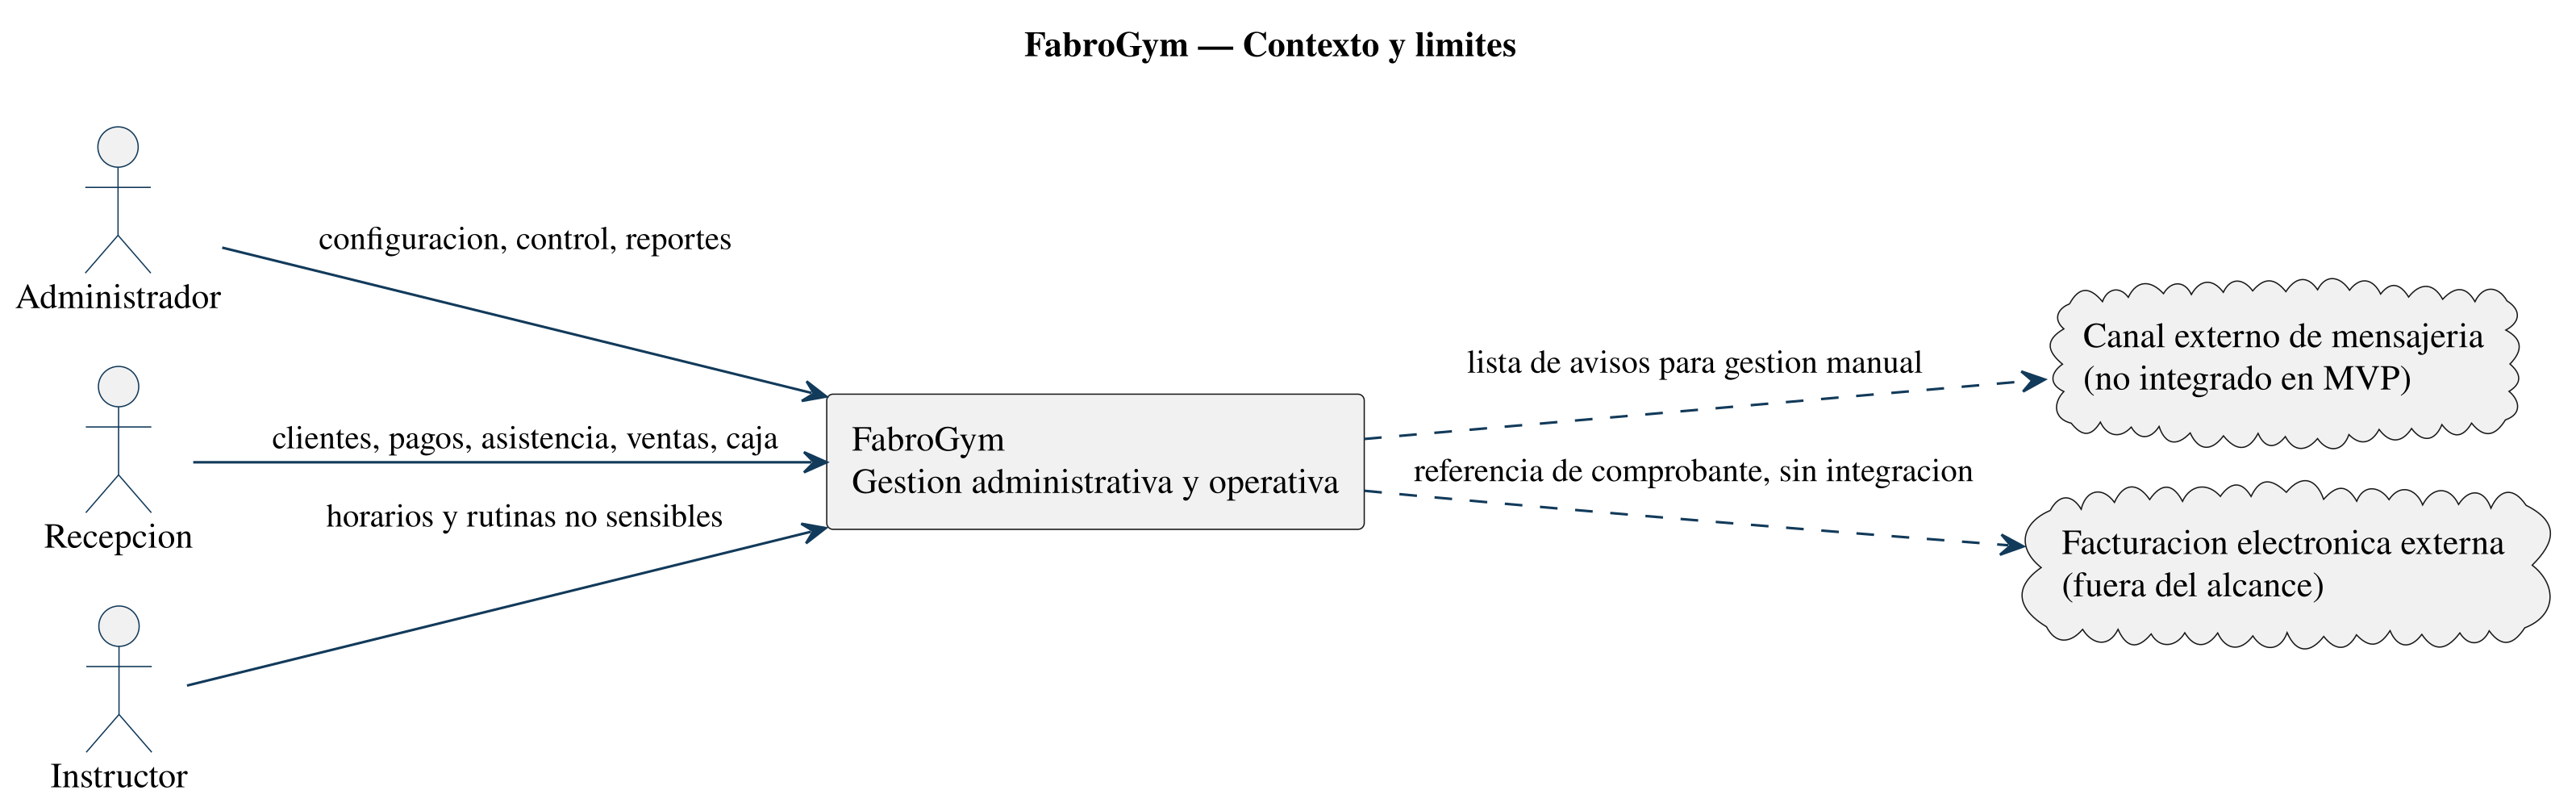
\includegraphics[width=.94\textwidth]{contexto.png}\caption{Contexto y frontera de FabroGym en la línea base de entrada.}\end{figure}

\section{ERS/SRS final integrado}
\subsection{Alcance y actores}
La línea base v2.0 incluye Superadministrador, Dueño, Recepcionista, Instructor y Cliente. Se incorporan consultas de autoservicio, configuración de IVA, categorías, proveedores, respaldo/restauración como requisitos de backend y dos componentes de IA como especificación futura. Permanecen fuera del alcance los diagnósticos, prescripciones médicas, biometría, peso y medidas corporales reales, nómina, banca y facturación electrónica integrada.

\subsection{Requisitos funcionales}
\begin{reqbox}{RF-AUT-01 - Autenticar usuario}
\begin{tabularx}{\textwidth}{>{\bfseries}p{3.2cm}Y}
Tipo y prioridad & Requisito funcional - Must \\
Actor & Personal autorizado \\
Fuente & EV-ENTR02-07 \\
Enunciado & El sistema deberá permitir iniciar y cerrar sesión mediante credenciales individuales no biométricas. \\
Caso de uso & CU-01 \\
Clases / proceso & Usuario; Rol; Permiso; EventoAuditoria; P-01 Controlar acceso \\
Estado & Aprobado en baseline v2.0 \\
\end{tabularx}
\textbf{Criterio BDD:} Dado un usuario con credenciales válidas, cuando inicie sesión, entonces el sistema deberá autenticarlo y habilitar únicamente las opciones permitidas para su rol; cuando cierre sesión, deberá invalidar la sesión activa.

\textbf{Trazas:} HU-01; CP-01; MU-01.
\end{reqbox}


\begin{reqbox}{RF-AUT-02 - Aplicar permisos por rol}
\begin{tabularx}{\textwidth}{>{\bfseries}p{3.2cm}Y}
Tipo y prioridad & Requisito funcional - Must \\
Actor & Administrador \\
Fuente & EV-ENTR02-07;EV-ENTR03-06;EV-ENTR08-04 \\
Enunciado & El sistema deberá autorizar cada operación según los roles Superadministrador, Dueño, Recepcionista, Instructor y Cliente, y deberá denegar por defecto toda operación no asignada. \\
Caso de uso & CU-02 \\
Clases / proceso & Usuario; Rol; Permiso; EventoAuditoria; P-01 Controlar acceso \\
Estado & Aprobado en baseline v2.0 \\
\end{tabularx}
\textbf{Criterio BDD:} Dado un usuario autenticado con un rol definido, cuando intente ejecutar una operación, entonces el sistema deberá permitirla solo si el permiso está asignado a ese rol y deberá denegarla en caso contrario.

\textbf{Trazas:} HU-02; CP-02; MU-22;MU-32.
\end{reqbox}


\begin{reqbox}{RF-AUT-03 - Auditar cambios criticos}
\begin{tabularx}{\textwidth}{>{\bfseries}p{3.2cm}Y}
Tipo y prioridad & Requisito funcional - Should \\
Actor & Administrador \\
Fuente & EV-ENTR02-04;EV-ENTR02-07;EV-ENTR03-06 \\
Enunciado & El sistema deberá registrar eventos de auditoría para cambios críticos en pagos, ventas, inventario, membresías, precios y permisos, incluyendo actor, fecha, acción, valor anterior y valor nuevo. \\
Caso de uso & CU-20 \\
Clases / proceso & Usuario; Rol; Permiso; EventoAuditoria; P-01 Controlar acceso \\
Estado & Aprobado en baseline v2.0 \\
\end{tabularx}
\textbf{Criterio BDD:} Dado un cambio crítico confirmado, cuando el sistema lo registre, entonces deberá conservar en auditoría el actor, fecha, acción, valor anterior y valor nuevo asociados al cambio.

\textbf{Trazas:} HU-20; CP-20; MU-25.
\end{reqbox}


\begin{reqbox}{RF-CLI-01 - Registrar cliente minimo}
\begin{tabularx}{\textwidth}{>{\bfseries}p{3.2cm}Y}
Tipo y prioridad & Requisito funcional - Must \\
Actor & Recepcionista \\
Fuente & EV-ENTR01-02;EV-ENTR02-02;EV-ENTR03-02;EV-ENTR08-01 \\
Enunciado & El sistema deberá registrar un cliente con código interno, nombre de uso y un medio de contacto, sin recopilar datos de salud, biometría, dirección domiciliaria ni imagen corporal. \\
Caso de uso & CU-03 \\
Clases / proceso & Cliente; Membresia; Pago; Asistencia; P-02 Gestionar clientes \\
Estado & Aprobado en baseline v2.0 \\
\end{tabularx}
\textbf{Criterio BDD:} Dado un formulario con código interno, nombre de uso y al menos un medio de contacto válido, cuando Recepción confirme el registro, entonces el sistema deberá crear un único cliente y no deberá solicitar datos de salud, biometría, dirección domiciliaria ni imagen corporal.

\textbf{Trazas:} HU-03; CP-03; MU-12*;MU-37*.
\end{reqbox}


\begin{reqbox}{RF-CLI-02 - Buscar y consultar cliente}
\begin{tabularx}{\textwidth}{>{\bfseries}p{3.2cm}Y}
Tipo y prioridad & Requisito funcional - Must \\
Actor & Recepcionista \\
Fuente & EV-ENTR02-03;EV-ENTR02-08;EV-ENTR08-05 \\
Enunciado & El sistema deberá buscar clientes por código, nombre normalizado o contacto y deberá mostrar membresía, último pago, asistencia y novedades de acuerdo con los permisos del usuario. \\
Caso de uso & CU-04 \\
Clases / proceso & Cliente; Membresia; Pago; Asistencia; P-02 Gestionar clientes \\
Estado & Aprobado en baseline v2.0 \\
\end{tabularx}
\textbf{Criterio BDD:} Dado un criterio de búsqueda válido, cuando Recepción consulte un cliente, entonces el sistema deberá devolver las coincidencias y mostrar únicamente membresía, último pago, asistencia y novedades autorizadas por el rol.

\textbf{Trazas:} HU-04; CP-04; MU-11;MU-36.
\end{reqbox}


\begin{reqbox}{RF-CLI-03 - Actualizar o reactivar sin duplicar}
\begin{tabularx}{\textwidth}{>{\bfseries}p{3.2cm}Y}
Tipo y prioridad & Requisito funcional - Must \\
Actor & Recepcionista \\
Fuente & EV-ENTR02-02;EV-ENTR03-02;EV-ENTR04-01;EV-ENTR05-02 \\
Enunciado & El sistema deberá actualizar o reactivar un registro existente y deberá advertir coincidencias antes de crear un cliente nuevo. \\
Caso de uso & CU-05 \\
Clases / proceso & Cliente; Membresia; Pago; Asistencia; P-02 Gestionar clientes \\
Estado & Aprobado en baseline v2.0 \\
\end{tabularx}
\textbf{Criterio BDD:} Dado que existe un cliente coincidente por código o contacto, cuando Recepción intente registrar o reactivar el perfil, entonces el sistema deberá advertir la coincidencia y permitir actualizar o reactivar el registro existente sin crear un duplicado.

\textbf{Trazas:} HU-05; CP-05; MU-11;MU-36.
\end{reqbox}


\begin{reqbox}{RF-MEM-01 - Configurar planes y promociones}
\begin{tabularx}{\textwidth}{>{\bfseries}p{3.2cm}Y}
Tipo y prioridad & Requisito funcional - Must \\
Actor & Administrador \\
Fuente & EV-ENTR02-01;EV-ENTR04-01 \\
Enunciado & El sistema deberá administrar el nombre, duración, precio, vigencia y estado de los planes y promociones. \\
Caso de uso & CU-06 \\
Clases / proceso & Membresia; Plan; Promocion; P-03 Gestionar membresías \\
Estado & Aprobado en baseline v2.0 \\
\end{tabularx}
\textbf{Criterio BDD:} Dado un usuario autorizado y los datos obligatorios de un plan o promoción, cuando guarde la configuración, entonces el sistema deberá conservar nombre, duración, precio, vigencia y estado y deberá mostrar el registro actualizado.

\textbf{Trazas:} HU-06; CP-06; MU-68.
\end{reqbox}


\begin{reqbox}{RF-MEM-02 - Activar o renovar membresia}
\begin{tabularx}{\textwidth}{>{\bfseries}p{3.2cm}Y}
Tipo y prioridad & Requisito funcional - Must \\
Actor & Recepcionista \\
Fuente & EV-ENTR01-02;EV-ENTR02-04;EV-ENTR03-01;EV-ENTR04-03 \\
Enunciado & El sistema deberá activar o renovar una membresía calculando las fechas de inicio y vencimiento a partir de un plan vigente y un pago confirmado. \\
Caso de uso & CU-07 \\
Clases / proceso & Membresia; Plan; Promocion; P-03 Gestionar membresías \\
Estado & Aprobado en baseline v2.0 \\
\end{tabularx}
\textbf{Criterio BDD:} Dado un plan vigente y un pago confirmado, cuando Recepción active o renueve la membresía, entonces el sistema deberá calcular y guardar las fechas de inicio y vencimiento según la duración del plan.

\textbf{Trazas:} HU-07; CP-07; MU-14;MU-39.
\end{reqbox}


\begin{reqbox}{RF-MEM-03 - Consultar vigencia}
\begin{tabularx}{\textwidth}{>{\bfseries}p{3.2cm}Y}
Tipo y prioridad & Requisito funcional - Must \\
Actor & Personal autorizado \\
Fuente & EV-ENTR01-03;EV-ENTR02-03;EV-ENTR03-03;EV-ENTR08-02 \\
Enunciado & El sistema deberá mostrar el estado, plan, fecha de inicio y fecha de vencimiento de la membresía. \\
Caso de uso & CU-08 \\
Clases / proceso & Membresia; Plan; Promocion; P-03 Gestionar membresías \\
Estado & Aprobado en baseline v2.0 \\
\end{tabularx}
\textbf{Criterio BDD:} Dado un cliente con membresía registrada, cuando un usuario autorizado consulte su vigencia, entonces el sistema deberá mostrar estado, plan, fecha de inicio y fecha de vencimiento de la membresía seleccionada.

\textbf{Trazas:} HU-08; CP-08; MU-13;MU-38;MU-63(F).
\end{reqbox}


\begin{reqbox}{RF-MEM-04 - Alertar vencimientos}
\begin{tabularx}{\textwidth}{>{\bfseries}p{3.2cm}Y}
Tipo y prioridad & Requisito funcional - Must \\
Actor & Recepcionista \\
Fuente & EV-ENTR01-03;EV-ENTR05-02;EV-ENTR07-02 \\
Enunciado & El sistema deberá listar diariamente las membresías que vencen en los próximos tres días y las membresías vencidas, sin enviar mensajes externos automáticamente. \\
Caso de uso & CU-09 \\
Clases / proceso & Membresia; Plan; Promocion; P-03 Gestionar membresías \\
Estado & Aprobado en baseline v2.0 \\
\end{tabularx}
\textbf{Criterio BDD:} Dado que existen membresías próximas a vencer o vencidas, cuando se ejecute la consulta diaria, entonces el sistema deberá separar las que vencen dentro de tres días de las ya vencidas y no deberá enviar mensajes externos de forma automática.

\textbf{Trazas:} HU-09; CP-09; MU-10;MU-13;MU-38.
\end{reqbox}


\begin{reqbox}{RF-PAG-01 - Registrar pago y comprobante}
\begin{tabularx}{\textwidth}{>{\bfseries}p{3.2cm}Y}
Tipo y prioridad & Requisito funcional - Must \\
Actor & Recepcionista \\
Fuente & EV-ENTR01-02;EV-ENTR02-04;EV-ENTR03-04;EV-ENTR07-02;EV-ENTR08-03 \\
Enunciado & El sistema deberá registrar monto, concepto, medio, referencia y fecha de un pago, y deberá generar un comprobante interno. \\
Caso de uso & CU-10 \\
Clases / proceso & Pago; Comprobante; Cliente; P-04 Gestionar pagos \\
Estado & Aprobado en baseline v2.0 \\
\end{tabularx}
\textbf{Criterio BDD:} Dado un pago con monto, concepto, medio, referencia y fecha válidos, cuando Recepción confirme el registro, entonces el sistema deberá guardar el pago y generar un comprobante interno vinculado al cliente.

\textbf{Trazas:} HU-10; CP-10; MU-15;MU-16;MU-40;MU-41.
\end{reqbox}


\begin{reqbox}{RF-PAG-02 - Resolver pago pendiente}
\begin{tabularx}{\textwidth}{>{\bfseries}p{3.2cm}Y}
Tipo y prioridad & Requisito funcional - Should \\
Actor & Administrador \\
Fuente & EV-ENTR02-04;EV-ENTR03-04;EV-ENTR07-07 \\
Enunciado & El sistema deberá permitir confirmar, rechazar o corregir un pago pendiente, conservando el motivo y el registro de auditoría. \\
Caso de uso & CU-21 \\
Clases / proceso & Pago; Comprobante; Cliente; P-04 Gestionar pagos \\
Estado & Aprobado en baseline v2.0 \\
\end{tabularx}
\textbf{Criterio BDD:} Dado un pago con estado pendiente, cuando un Administrador lo confirme, rechace o corrija, entonces el sistema deberá actualizar el estado y conservar el motivo y la evidencia de auditoría de la decisión.

\textbf{Trazas:} HU-21; CP-21; MU-15;MU-40.
\end{reqbox}


\begin{reqbox}{RF-ASI-01 - Registrar asistencia}
\begin{tabularx}{\textwidth}{>{\bfseries}p{3.2cm}Y}
Tipo y prioridad & Requisito funcional - Must \\
Actor & Recepcionista \\
Fuente & EV-ENTR02-03;EV-ENTR03-03;EV-ENTR04-02;EV-ENTR07-07;EV-ENTR08-02 \\
Enunciado & El sistema deberá registrar asistencia mediante código QR como flujo normal y deberá disponer de registro manual como contingencia autorizada, conservando método, responsable, fecha y motivo. \\
Caso de uso & CU-11 \\
Clases / proceso & Asistencia; Cliente; Turno; P-05 Controlar asistencia \\
Estado & Aprobado en baseline v2.0 \\
\end{tabularx}
\textbf{Criterio BDD:} Dado un cliente identificado, cuando Recepción registre la asistencia por QR, entonces el sistema deberá guardar fecha, hora y método QR; si se utiliza contingencia manual, deberá exigir responsable y motivo.

\textbf{Trazas:} HU-11; CP-11; MU-20;MU-30*;MU-46;MU-47*.
\end{reqbox}


\begin{reqbox}{RF-ASI-02 - Consultar asistencia}
\begin{tabularx}{\textwidth}{>{\bfseries}p{3.2cm}Y}
Tipo y prioridad & Requisito funcional - Must \\
Actor & Personal autorizado \\
Fuente & EV-ENTR03-01;EV-ENTR07-01;EV-ENTR08-05;EV-ENTR09-06 \\
Enunciado & El sistema deberá filtrar asistencias por cliente, fecha y turno, y deberá mostrar los conteos operativos correspondientes. \\
Caso de uso & CU-12 \\
Clases / proceso & Asistencia; Cliente; Turno; P-05 Controlar asistencia \\
Estado & Aprobado en baseline v2.0 \\
\end{tabularx}
\textbf{Criterio BDD:} Dado un filtro por cliente, fecha o turno, cuando un usuario autorizado consulte asistencias, entonces el sistema deberá mostrar únicamente los registros que cumplan el filtro y los conteos correspondientes.

\textbf{Trazas:} HU-12; CP-12; MU-20;MU-46;MU-56;MU-65(F).
\end{reqbox}


\begin{reqbox}{RF-INV-01 - Administrar productos}
\begin{tabularx}{\textwidth}{>{\bfseries}p{3.2cm}Y}
Tipo y prioridad & Requisito funcional - Must \\
Actor & Administrador \\
Fuente & EV-ENTR01-01;EV-ENTR02-05 \\
Enunciado & El sistema deberá registrar productos con código, nombre, precio, unidad, stock mínimo y estado. \\
Caso de uso & CU-13 \\
Clases / proceso & Producto; Categoria; Proveedor; MovimientoStock; P-06 Gestionar inventario \\
Estado & Aprobado en baseline v2.0 \\
\end{tabularx}
\textbf{Criterio BDD:} Dado un producto con código, nombre, precio, unidad, stock mínimo y estado válidos, cuando el Administrador confirme el registro, entonces el sistema deberá guardar el producto y permitir su consulta posterior.

\textbf{Trazas:} HU-13; CP-13; MU-19;MU-28;MU-44*;MU-45*.
\end{reqbox}


\begin{reqbox}{RF-INV-02 - Registrar movimientos de stock}
\begin{tabularx}{\textwidth}{>{\bfseries}p{3.2cm}Y}
Tipo y prioridad & Requisito funcional - Must \\
Actor & Personal autorizado \\
Fuente & EV-ENTR01-04;EV-ENTR04-04;EV-ENTR07-03 \\
Enunciado & El sistema deberá registrar entradas y ajustes de inventario con cantidad, motivo, responsable y saldo resultante. \\
Caso de uso & CU-14 \\
Clases / proceso & Producto; Categoria; Proveedor; MovimientoStock; P-06 Gestionar inventario \\
Estado & Aprobado en baseline v2.0 \\
\end{tabularx}
\textbf{Criterio BDD:} Dado un producto existente y un movimiento válido, cuando un usuario autorizado registre una entrada o ajuste, entonces el sistema deberá actualizar el saldo y conservar cantidad, motivo, responsable y saldo resultante.

\textbf{Trazas:} HU-14; CP-14; MU-69.
\end{reqbox}


\begin{reqbox}{RF-VEN-01 - Registrar venta}
\begin{tabularx}{\textwidth}{>{\bfseries}p{3.2cm}Y}
Tipo y prioridad & Requisito funcional - Must \\
Actor & Recepcionista \\
Fuente & EV-ENTR02-05;EV-ENTR03-01;EV-ENTR04-04;EV-ENTR07-03;EV-ENTR08-03 \\
Enunciado & El sistema deberá registrar una venta con sus ítems y medio de pago, y deberá descontar las existencias en la misma transacción. \\
Caso de uso & CU-15 \\
Clases / proceso & Venta; DetalleVenta; Producto; Pago; P-07 Registrar ventas \\
Estado & Aprobado en baseline v2.0 \\
\end{tabularx}
\textbf{Criterio BDD:} Dado que todos los ítems de una venta tienen stock suficiente, cuando Recepción confirme la venta, entonces el sistema deberá registrar la venta y descontar las existencias en una única transacción; si falla una operación, no deberá aplicar cambios parciales.

\textbf{Trazas:} HU-15; CP-15; MU-18;MU-27;MU-42;MU-43.
\end{reqbox}


\begin{reqbox}{RF-INV-03 - Alertar stock y rotacion}
\begin{tabularx}{\textwidth}{>{\bfseries}p{3.2cm}Y}
Tipo y prioridad & Requisito funcional - Should \\
Actor & Administrador \\
Fuente & EV-ENTR01-04;EV-ENTR02-05;EV-ENTR05-04;EV-ENTR06-04 \\
Enunciado & El sistema deberá listar los productos cuyo stock sea igual o inferior al stock mínimo y deberá resumir entradas, salidas y ventas por período. \\
Caso de uso & CU-22 \\
Clases / proceso & Producto; Categoria; Proveedor; MovimientoStock; P-06 Gestionar inventario \\
Estado & Aprobado en baseline v2.0 \\
\end{tabularx}
\textbf{Criterio BDD:} Dado un período de consulta, cuando el Administrador solicite el control de stock, entonces el sistema deberá listar los productos con stock igual o inferior al mínimo y resumir entradas, salidas y ventas del período.

\textbf{Trazas:} HU-22; CP-22; MU-10;MU-19;MU-44*.
\end{reqbox}


\begin{reqbox}{RF-CAJ-01 - Cerrar turno y conciliar caja}
\begin{tabularx}{\textwidth}{>{\bfseries}p{3.2cm}Y}
Tipo y prioridad & Requisito funcional - Must \\
Actor & Recepcionista \\
Fuente & EV-ENTR02-01;EV-ENTR02-06;EV-ENTR03-05;EV-ENTR04-05;EV-ENTR07-03;EV-ENTR08-04 \\
Enunciado & El sistema deberá calcular pagos y ventas por medio de pago, comparar los valores declarados y registrar las diferencias y la entrega de turno. \\
Caso de uso & CU-16 \\
Clases / proceso & Caja; Turno; Venta; Pago; P-08 Conciliar caja \\
Estado & Aprobado en baseline v2.0 \\
\end{tabularx}
\textbf{Criterio BDD:} Dado un turno con pagos y ventas registrados, cuando Recepción ejecute el cierre, entonces el sistema deberá totalizar por medio de pago, comparar contra los valores declarados y registrar cualquier diferencia junto con la entrega del turno.

\textbf{Trazas:} HU-16; CP-16; MU-70.
\end{reqbox}


\begin{reqbox}{RF-NOV-01 - Gestionar novedades internas}
\begin{tabularx}{\textwidth}{>{\bfseries}p{3.2cm}Y}
Tipo y prioridad & Requisito funcional - Must \\
Actor & Personal autorizado \\
Fuente & EV-ENTR02-01;EV-ENTR02-08;EV-ENTR03-07;EV-ENTR04-06;EV-ENTR05-01 \\
Enunciado & El sistema deberá crear una novedad con categoría, detalle mínimo, responsable, vencimiento y uno de los estados: pendiente, en proceso, resuelta o cancelada. \\
Caso de uso & CU-17 \\
Clases / proceso & Novedad; Usuario; P-09 Gestionar novedades \\
Estado & Aprobado en baseline v2.0 \\
\end{tabularx}
\textbf{Criterio BDD:} Dado un usuario autorizado y una novedad con categoría, detalle, responsable y vencimiento, cuando la registre, entonces el sistema deberá crearla con un estado válido y conservar los cambios posteriores de estado.

\textbf{Trazas:} HU-17; CP-17; MU-21;MU-31*;MU-50;MU-51*;MU-61.
\end{reqbox}


\begin{reqbox}{RF-INS-01 - Gestionar horario y disponibilidad de instructor}
\begin{tabularx}{\textwidth}{>{\bfseries}p{3.2cm}Y}
Tipo y prioridad & Requisito funcional - Should \\
Actor & Administrador \\
Fuente & EV-ENTR07-06;EV-ENTR09-03;EV-ENTR10-02 \\
Enunciado & El sistema deberá registrar turnos, capacidad, disponibilidad y novedades operativas del instructor, sin recopilar datos de salud. \\
Caso de uso & CU-23 \\
Clases / proceso & Instructor; Horario; Cliente; P-10 Gestionar instructores \\
Estado & Aprobado en baseline v2.0 \\
\end{tabularx}
\textbf{Criterio BDD:} Dado un instructor registrado, cuando el Administrador actualice su operación, entonces el sistema deberá guardar turnos, capacidad, disponibilidad y novedades operativas sin solicitar datos de salud.

\textbf{Trazas:} HU-23; CP-23; MU-23;MU-33;MU-48*;MU-49*;MU-58.
\end{reqbox}


\begin{reqbox}{RF-RUT-01 - Crear y asignar rutina}
\begin{tabularx}{\textwidth}{>{\bfseries}p{3.2cm}Y}
Tipo y prioridad & Requisito funcional - Must \\
Actor & Instructor \\
Fuente & EV-ENTR01-05;EV-ENTR05-04;EV-ENTR09-01;EV-ENTR09-02;EV-ENTR09-03 \\
Enunciado & El sistema deberá crear una rutina con objetivo operativo, ejercicios, series, repeticiones, descanso y días de ejecución, y deberá asignarla a un cliente autorizado. \\
Caso de uso & CU-18 \\
Clases / proceso & Rutina; VersionRutina; Ejercicio; Cliente; Instructor; P-11 Gestionar rutinas \\
Estado & Aprobado en baseline v2.0 \\
\end{tabularx}
\textbf{Criterio BDD:} Dado un cliente autorizado y un catálogo de ejercicios disponible, cuando el Instructor cree una rutina, entonces el sistema deberá guardar objetivo operativo, ejercicios, series, repeticiones, descanso y días, y deberá asignarla al cliente seleccionado.

\textbf{Trazas:} HU-18; CP-18; MU-17*;MU-29*;MU-54;MU-55;MU-64(F).
\end{reqbox}


\begin{reqbox}{RF-RUT-02 - Versionar y ajustar rutina}
\begin{tabularx}{\textwidth}{>{\bfseries}p{3.2cm}Y}
Tipo y prioridad & Requisito funcional - Must \\
Actor & Instructor \\
Fuente & EV-ENTR01-05;EV-ENTR09-01;EV-ENTR09-04;EV-ENTR10-01;EV-ENTR10-03 \\
Enunciado & El sistema deberá crear una nueva versión cuando se modifiquen ejercicios o parámetros de una rutina y deberá conservar las versiones anteriores en modo de solo lectura. \\
Caso de uso & CU-19 \\
Clases / proceso & Rutina; VersionRutina; Ejercicio; Cliente; Instructor; P-11 Gestionar rutinas \\
Estado & Aprobado en baseline v2.0 \\
\end{tabularx}
\textbf{Criterio BDD:} Dado una rutina existente, cuando el Instructor modifique ejercicios o parámetros y confirme el cambio, entonces el sistema deberá crear una nueva versión y mantener las versiones anteriores en solo lectura.

\textbf{Trazas:} HU-19; CP-19; MU-17*;MU-54.
\end{reqbox}


\begin{reqbox}{RF-RUT-03 - Registrar seguimiento operativo}
\begin{tabularx}{\textwidth}{>{\bfseries}p{3.2cm}Y}
Tipo y prioridad & Requisito funcional - Should \\
Actor & Instructor \\
Fuente & EV-ENTR09-04;EV-ENTR09-05;EV-ENTR09-06;EV-ENTR10-03;EV-ENTR10-04 \\
Enunciado & El sistema deberá registrar fecha, cumplimiento de ejercicios, repeticiones y observación operativa, excluyendo diagnósticos, lesiones, peso y medidas corporales reales. \\
Caso de uso & CU-24 \\
Clases / proceso & Rutina; VersionRutina; Ejercicio; Cliente; Instructor; P-11 Gestionar rutinas \\
Estado & Aprobado en baseline v2.0 \\
\end{tabularx}
\textbf{Criterio BDD:} Dado una rutina activa, cuando el Instructor registre seguimiento, entonces el sistema deberá guardar fecha, cumplimiento, repeticiones y observación operativa y deberá rechazar campos destinados a diagnósticos, lesiones, peso o medidas corporales reales.

\textbf{Trazas:} HU-24; CP-24; MU-59;MU-60*.
\end{reqbox}


\begin{reqbox}{RF-REP-01 - Consultar panel y reportes}
\begin{tabularx}{\textwidth}{>{\bfseries}p{3.2cm}Y}
Tipo y prioridad & Requisito funcional - Should \\
Actor & Administrador \\
Fuente & EV-ENTR01-05;EV-ENTR05-05;EV-ENTR06-04;EV-ENTR07-04;EV-ENTR08-05;EV-ENTR09-05 \\
Enunciado & El sistema deberá mostrar indicadores filtrables de clientes, membresías, ventas, asistencias, uso y promociones por período, calculados exclusivamente con datos almacenados y exportables a CSV. \\
Caso de uso & CU-25 \\
Clases / proceso & Reporte; Indicador; Filtro; P-12 Generar reportes \\
Estado & Aprobado en baseline v2.0 \\
\end{tabularx}
\textbf{Criterio BDD:} Dado un período y filtros válidos, cuando el Administrador consulte el panel o reporte, entonces el sistema deberá calcular los indicadores con datos almacenados, mostrar los resultados filtrados y permitir exportarlos a CSV.

\textbf{Trazas:} HU-25; CP-25; MU-10;MU-24;MU-34.
\end{reqbox}


\begin{reqbox}{RF-MEM-05 - Consultar mi membresía}
\begin{tabularx}{\textwidth}{>{\bfseries}p{3.2cm}Y}
Tipo y prioridad & Requisito funcional - Must \\
Actor & Cliente \\
Fuente & EV-VT-T02-12; MU-63 \\
Enunciado & El sistema deberá permitir al cliente autenticado consultar el estado, plan y vigencia de su propia membresía en modo de solo lectura. \\
Caso de uso & CU-26 \\
Clases / proceso & Membresia; Plan; Promocion; P-03 Gestionar membresías \\
Estado & Aprobado en baseline v2.0 \\
\end{tabularx}
\textbf{Criterio BDD:} Dado un Cliente autenticado, cuando consulte su membresía, entonces el sistema deberá mostrar únicamente el estado, plan y vigencia de su propia membresía y no deberá habilitar edición.

\textbf{Trazas:} HU-26; CP-26; V7 / modelo conceptual.
\end{reqbox}


\begin{reqbox}{RF-PAG-03 - Consultar mis pagos}
\begin{tabularx}{\textwidth}{>{\bfseries}p{3.2cm}Y}
Tipo y prioridad & Requisito funcional - Must \\
Actor & Cliente \\
Fuente & EV-VT-T02-12 \\
Enunciado & El sistema deberá permitir al cliente autenticado consultar sus pagos registrados y el estado contextual de cada pago en modo de solo lectura. \\
Caso de uso & CU-27 \\
Clases / proceso & Pago; Comprobante; Cliente; P-04 Gestionar pagos \\
Estado & Aprobado en baseline v2.0 \\
\end{tabularx}
\textbf{Criterio BDD:} Dado un Cliente autenticado, cuando consulte sus pagos, entonces el sistema deberá mostrar únicamente sus registros de pago y el estado de cada uno en modo de solo lectura.

\textbf{Trazas:} HU-27; CP-27; V7 / modelo conceptual.
\end{reqbox}


\begin{reqbox}{RF-RUT-04 - Consultar mi rutina e historial}
\begin{tabularx}{\textwidth}{>{\bfseries}p{3.2cm}Y}
Tipo y prioridad & Requisito funcional - Must \\
Actor & Cliente \\
Fuente & EV-VT-T01-06; EV-VT-T01-08; EV-VT-T02-04 \\
Enunciado & El sistema deberá permitir al cliente autenticado consultar su rutina activa, sus versiones y el seguimiento operativo autorizado, sin modificar la rutina vigente. \\
Caso de uso & CU-28 \\
Clases / proceso & Rutina; VersionRutina; Ejercicio; Cliente; Instructor; P-11 Gestionar rutinas \\
Estado & Aprobado en baseline v2.0 \\
\end{tabularx}
\textbf{Criterio BDD:} Dado un Cliente autenticado con una rutina asignada, cuando consulte su rutina, entonces el sistema deberá mostrar la versión activa, las versiones históricas y el seguimiento autorizado sin permitir modificar la rutina vigente.

\textbf{Trazas:} HU-28; CP-28; V7 / modelo conceptual.
\end{reqbox}


\begin{reqbox}{RF-INV-04 - Gestionar categorías de productos}
\begin{tabularx}{\textwidth}{>{\bfseries}p{3.2cm}Y}
Tipo y prioridad & Requisito funcional - Should \\
Actor & Dueño \\
Fuente & EV-VT-T03-06 \\
Enunciado & El sistema deberá permitir al usuario autorizado registrar, consultar, editar y desactivar categorías de productos. \\
Caso de uso & CU-29 \\
Clases / proceso & Producto; Categoria; Proveedor; MovimientoStock; P-06 Gestionar inventario \\
Estado & Aprobado en baseline v2.0 \\
\end{tabularx}
\textbf{Criterio BDD:} Dado un usuario autorizado, cuando registre, edite o desactive una categoría, entonces el sistema deberá guardar el cambio y reflejar el estado actualizado en las consultas de categorías.

\textbf{Trazas:} HU-29; CP-29; V7 / modelo conceptual.
\end{reqbox}


\begin{reqbox}{RF-INV-05 - Gestionar proveedores}
\begin{tabularx}{\textwidth}{>{\bfseries}p{3.2cm}Y}
Tipo y prioridad & Requisito funcional - Should \\
Actor & Dueño \\
Fuente & EV-VT-T03-06; EV-VT-T01-10 \\
Enunciado & El sistema deberá permitir al usuario autorizado registrar, consultar, editar y desactivar proveedores utilizados en inventario. \\
Caso de uso & CU-30 \\
Clases / proceso & Producto; Categoria; Proveedor; MovimientoStock; P-06 Gestionar inventario \\
Estado & Aprobado en baseline v2.0 \\
\end{tabularx}
\textbf{Criterio BDD:} Dado un usuario autorizado, cuando registre, edite o desactive un proveedor, entonces el sistema deberá guardar el cambio y reflejar el estado actualizado en las consultas de proveedores.

\textbf{Trazas:} HU-30; CP-30; V7 / modelo conceptual.
\end{reqbox}


\begin{reqbox}{RF-CFG-01 - Configurar tratamiento de IVA}
\begin{tabularx}{\textwidth}{>{\bfseries}p{3.2cm}Y}
Tipo y prioridad & Requisito funcional - Must \\
Actor & Dueño \\
Fuente & EV-VT-T03-05 \\
Enunciado & El sistema deberá permitir configurar el porcentaje general de IVA y definir por producto si el impuesto aplica, conservando el historial de cambios. \\
Caso de uso & CU-31 \\
Clases / proceso & Configuracion; HorarioAtencion; Producto; P-13 Configurar operación \\
Estado & Aprobado en baseline v2.0 \\
\end{tabularx}
\textbf{Criterio BDD:} Dado un porcentaje de IVA válido y la configuración tributaria de un producto, cuando el Dueño confirme el cambio, entonces el sistema deberá aplicar la nueva configuración a operaciones posteriores y conservar el valor anterior, el nuevo valor, el actor y la fecha.

\textbf{Trazas:} HU-31; CP-31; V7 / modelo conceptual.
\end{reqbox}


\begin{reqbox}{RF-BCK-01 - Generar respaldo}
\begin{tabularx}{\textwidth}{>{\bfseries}p{3.2cm}Y}
Tipo y prioridad & Requisito funcional - Should \\
Actor & Superadministrador \\
Fuente & EV-VT-T03-10 \\
Enunciado & El sistema deberá permitir iniciar un respaldo cifrado y consultar su estado y fecha de finalización. \\
Caso de uso & CU-32 \\
Clases / proceso & Respaldo; EventoAuditoria; P-14 Respaldar y recuperar \\
Estado & Aprobado en baseline v2.0 \\
\end{tabularx}
\textbf{Criterio BDD:} Dado un Superadministrador autenticado, cuando solicite un respaldo, entonces el sistema deberá iniciar el proceso cifrado, asignar un identificador y mostrar el estado y la fecha de finalización cuando concluya.

\textbf{Trazas:} HU-32; CP-32; V7 / modelo conceptual.
\end{reqbox}


\begin{reqbox}{RF-BCK-02 - Restaurar respaldo}
\begin{tabularx}{\textwidth}{>{\bfseries}p{3.2cm}Y}
Tipo y prioridad & Requisito funcional - Should \\
Actor & Superadministrador \\
Fuente & EV-VT-T03-10 \\
Enunciado & El sistema deberá permitir restaurar un respaldo seleccionado mediante confirmación explícita, verificación de integridad y registro de auditoría. \\
Caso de uso & CU-33 \\
Clases / proceso & Respaldo; EventoAuditoria; P-14 Respaldar y recuperar \\
Estado & Aprobado en baseline v2.0 \\
\end{tabularx}
\textbf{Criterio BDD:} Dado un respaldo íntegro seleccionado, cuando el Superadministrador confirme explícitamente la restauración, entonces el sistema deberá verificar su integridad, ejecutar la restauración y registrar la operación en auditoría; si la verificación falla, no deberá restaurar.

\textbf{Trazas:} HU-33; CP-33; V7 / modelo conceptual.
\end{reqbox}


\begin{reqbox}{RF-CFG-02 - Configurar horario de atención}
\begin{tabularx}{\textwidth}{>{\bfseries}p{3.2cm}Y}
Tipo y prioridad & Requisito funcional - Could \\
Actor & Dueño \\
Fuente & IND-14; V7 \\
Enunciado & El sistema deberá permitir configurar los días y horas de atención del gimnasio y deberá mostrarlos al cliente. \\
Caso de uso & CU-34 \\
Clases / proceso & Configuracion; HorarioAtencion; Producto; P-13 Configurar operación \\
Estado & Aprobado en baseline v2.0 \\
\end{tabularx}
\textbf{Criterio BDD:} Dado un Dueño autenticado y una configuración válida de días y horas, cuando guarde el horario, entonces el sistema deberá actualizarlo y mostrar al Cliente únicamente el horario vigente.

\textbf{Trazas:} HU-34; CP-34; V7 / modelo conceptual.
\end{reqbox}


\begin{reqbox}{RF-IA-RUT-01 - Generar recomendación de rutina}
\begin{tabularx}{\textwidth}{>{\bfseries}p{3.2cm}Y}
Tipo y prioridad & Requisito funcional - Must \\
Actor & Cliente/Instructor \\
Fuente & EV-VT-T02-05; H03; PE5-OE3 \\
Enunciado & El sistema deberá generar hasta tres alternativas de rutina a partir del objetivo declarado, la disponibilidad semanal, el historial operativo no sensible y el catálogo de ejercicios autorizado. \\
Caso de uso & CU-35 \\
Clases / proceso & ModeloIA; Recomendacion; Alerta; Explicacion; P-15 Asistir decisiones \\
Estado & Aprobado como requisito PE5; implementación pendiente \\
\end{tabularx}
\textbf{Criterio BDD:} Dado un objetivo operativo, disponibilidad semanal, historial no sensible y catálogo autorizado, cuando se solicite una recomendación, entonces el componente deberá devolver como máximo tres alternativas ordenadas de rutina y una explicación de los factores utilizados.

\textbf{Trazas:} HU-35; CP-35; Prototipo pendiente.
\end{reqbox}


\begin{reqbox}{RF-IA-RUT-02 - Aceptar, rechazar o solicitar alternativa}
\begin{tabularx}{\textwidth}{>{\bfseries}p{3.2cm}Y}
Tipo y prioridad & Requisito funcional - Must \\
Actor & Cliente \\
Fuente & Decisión del equipo; PE5-OE3 \\
Enunciado & El sistema deberá permitir aceptar, rechazar o solicitar una alternativa antes de incorporar una recomendación a la propuesta de rutina. \\
Caso de uso & CU-36 \\
Clases / proceso & ModeloIA; Recomendacion; Alerta; Explicacion; P-15 Asistir decisiones \\
Estado & Aprobado como requisito PE5; implementación pendiente \\
\end{tabularx}
\textbf{Criterio BDD:} Dado que el Cliente visualiza una recomendación de rutina, cuando seleccione aceptar, rechazar o solicitar alternativa, entonces el sistema deberá registrar la decisión y no deberá activar automáticamente la recomendación.

\textbf{Trazas:} HU-36; CP-36; Prototipo pendiente.
\end{reqbox}


\begin{reqbox}{RF-IA-RUT-03 - Revisar recomendación de rutina}
\begin{tabularx}{\textwidth}{>{\bfseries}p{3.2cm}Y}
Tipo y prioridad & Requisito funcional - Must \\
Actor & Instructor \\
Fuente & EV-VT-T01-07; EV-VT-T01-08; H02 \\
Enunciado & El sistema deberá exigir la revisión del instructor antes de activar una rutina recomendada y deberá conservar la decisión y el motivo. \\
Caso de uso & CU-37 \\
Clases / proceso & ModeloIA; Recomendacion; Alerta; Explicacion; P-15 Asistir decisiones \\
Estado & Aprobado como requisito PE5; implementación pendiente \\
\end{tabularx}
\textbf{Criterio BDD:} Dado una recomendación aceptada por el Cliente, cuando el Instructor la revise, entonces el sistema deberá permitir aprobarla o rechazarla con motivo; únicamente una aprobación explícita podrá habilitar su activación.

\textbf{Trazas:} HU-37; CP-37; Prototipo pendiente.
\end{reqbox}


\begin{reqbox}{RF-IA-ABA-01 - Calcular riesgo de inactividad}
\begin{tabularx}{\textwidth}{>{\bfseries}p{3.2cm}Y}
Tipo y prioridad & Requisito funcional - Should \\
Actor & Dueño \\
Fuente & PE5-OE3; decisión de diseño \\
Enunciado & El sistema deberá calcular semanalmente un nivel de riesgo bajo, medio o alto usando únicamente asistencia, vigencia de membresía y frecuencia histórica. \\
Caso de uso & CU-38 \\
Clases / proceso & ModeloIA; Recomendacion; Alerta; Explicacion; P-15 Asistir decisiones \\
Estado & Aprobado como requisito PE5; implementación pendiente \\
\end{tabularx}
\textbf{Criterio BDD:} Dado el historial de asistencia, vigencia de membresía y frecuencia histórica de un cliente, cuando se ejecute el cálculo semanal, entonces el componente deberá asignar un nivel bajo, medio o alto y registrar la fecha del cálculo.

\textbf{Trazas:} HU-38; CP-38; Prototipo pendiente.
\end{reqbox}


\begin{reqbox}{RF-IA-ABA-02 - Mostrar alertas de riesgo}
\begin{tabularx}{\textwidth}{>{\bfseries}p{3.2cm}Y}
Tipo y prioridad & Requisito funcional - Should \\
Actor & Dueño/Recepcionista \\
Fuente & PE5-OE3; decisión de diseño \\
Enunciado & El sistema deberá mostrar los clientes con riesgo medio o alto, los factores principales y la fecha del cálculo, sin ejecutar acciones automáticas. \\
Caso de uso & CU-39 \\
Clases / proceso & ModeloIA; Recomendacion; Alerta; Explicacion; P-15 Asistir decisiones \\
Estado & Aprobado como requisito PE5; implementación pendiente \\
\end{tabularx}
\textbf{Criterio BDD:} Dado que existen clientes clasificados con riesgo medio o alto, cuando Dueño o Recepcionista consulte las alertas, entonces el sistema deberá mostrar el nivel, la fecha y los principales factores de cada alerta sin ejecutar acciones automáticas.

\textbf{Trazas:} HU-39; CP-39; Prototipo pendiente.
\end{reqbox}


\begin{reqbox}{RF-IA-ABA-03 - Registrar seguimiento de alerta}
\begin{tabularx}{\textwidth}{>{\bfseries}p{3.2cm}Y}
Tipo y prioridad & Requisito funcional - Should \\
Actor & Recepcionista \\
Fuente & PE5-OE3; decisión de diseño \\
Enunciado & El sistema deberá permitir registrar el contacto, aplazamiento o descarte de una alerta y deberá conservar la decisión humana para auditoría. \\
Caso de uso & CU-40 \\
Clases / proceso & ModeloIA; Recomendacion; Alerta; Explicacion; P-15 Asistir decisiones \\
Estado & Aprobado como requisito PE5; implementación pendiente \\
\end{tabularx}
\textbf{Criterio BDD:} Dado una alerta de riesgo visible, cuando Recepción registre contacto, aplazamiento o descarte, entonces el sistema deberá guardar la acción, responsable, fecha y observación para auditoría.

\textbf{Trazas:} HU-40; CP-40; Prototipo pendiente.
\end{reqbox}

\subsection{Requisitos no funcionales}

\begin{reqbox}[colframe=Teal]{RNF-AF-01 - Adecuación funcional}
\begin{tabularx}{\textwidth}{>{\bfseries}p{3.2cm}Y}
Tipo y prioridad & Requisito no funcional - Must \\
Fuente & ISO/IEC 25010:2023; PE5 \\
Enunciado medible & El 100 \% de los RF Must deberá disponer de criterio BDD y caso de prueba conceptual antes de liberar una línea base. \\
Método de comprobación & Prueba reproducible registrada en CP-RNF-AF-01 y contraste con el umbral del enunciado. \\
Estado & Especificado; verificación pendiente \\
\end{tabularx}
\textbf{Criterio BDD:} Dado un entorno de prueba reproducible, cuando se ejecute el método de comprobación definido para RNF-AF-01, entonces se deberá alcanzar el umbral expresado en el requisito y conservar la evidencia.
\end{reqbox}


\begin{reqbox}[colframe=Teal]{RNF-ED-01 - Rendimiento de consultas}
\begin{tabularx}{\textwidth}{>{\bfseries}p{3.2cm}Y}
Tipo y prioridad & Requisito no funcional - Must \\
Fuente & ISO/IEC 25010:2023 \\
Enunciado medible & Con 10 000 clientes sintéticos y 20 sesiones concurrentes, el percentil 95 de búsqueda y consulta será menor o igual a 5 s y la tasa de error menor o igual a 1 \%. \\
Método de comprobación & Prueba reproducible registrada en CP-RNF-ED-01 y contraste con el umbral del enunciado. \\
Estado & Especificado; verificación pendiente \\
\end{tabularx}
\textbf{Criterio BDD:} Dado un entorno de prueba reproducible, cuando se ejecute el método de comprobación definido para RNF-ED-01, entonces se deberá alcanzar el umbral expresado en el requisito y conservar la evidencia.
\end{reqbox}


\begin{reqbox}[colframe=Teal]{RNF-ED-02 - Tiempo de registro de asistencia}
\begin{tabularx}{\textwidth}{>{\bfseries}p{3.2cm}Y}
Tipo y prioridad & Requisito no funcional - Must \\
Fuente & EV-VT-T01-03; EV-VT-T02-06; EV-VT-T03-08 \\
Enunciado medible & Al menos 9 de 10 tareas moderadas de registro de asistencia deberán completarse en 30 s o menos. \\
Método de comprobación & Prueba reproducible registrada en CP-RNF-ED-02 y contraste con el umbral del enunciado. \\
Estado & Especificado; verificación pendiente \\
\end{tabularx}
\textbf{Criterio BDD:} Dado un entorno de prueba reproducible, cuando se ejecute el método de comprobación definido para RNF-ED-02, entonces se deberá alcanzar el umbral expresado en el requisito y conservar la evidencia.
\end{reqbox}


\begin{reqbox}[colframe=Teal]{RNF-COM-01 - Compatibilidad web}
\begin{tabularx}{\textwidth}{>{\bfseries}p{3.2cm}Y}
Tipo y prioridad & Requisito no funcional - Should \\
Fuente & ISO/IEC 25010:2023 \\
Enunciado medible & Las funciones Must deberán superar todas sus pruebas en las dos versiones estables más recientes de Chrome, Edge y Firefox disponibles al corte. \\
Método de comprobación & Prueba reproducible registrada en CP-RNF-COM-01 y contraste con el umbral del enunciado. \\
Estado & Especificado; verificación pendiente \\
\end{tabularx}
\textbf{Criterio BDD:} Dado un entorno de prueba reproducible, cuando se ejecute el método de comprobación definido para RNF-COM-01, entonces se deberá alcanzar el umbral expresado en el requisito y conservar la evidencia.
\end{reqbox}


\begin{reqbox}[colframe=Teal]{RNF-IU-01 - Usabilidad de tareas críticas}
\begin{tabularx}{\textwidth}{>{\bfseries}p{3.2cm}Y}
Tipo y prioridad & Requisito no funcional - Must \\
Fuente & EV-VT-T01-11; EV-VT-T01-12; H04; H05 \\
Enunciado medible & Al menos 9 de 10 tareas críticas deberán completarse sin ayuda por cada perfil en walkthrough moderado. \\
Método de comprobación & Prueba reproducible registrada en CP-RNF-IU-01 y contraste con el umbral del enunciado. \\
Estado & Especificado; verificación pendiente \\
\end{tabularx}
\textbf{Criterio BDD:} Dado un entorno de prueba reproducible, cuando se ejecute el método de comprobación definido para RNF-IU-01, entonces se deberá alcanzar el umbral expresado en el requisito y conservar la evidencia.
\end{reqbox}


\begin{reqbox}[colframe=Teal]{RNF-IU-02 - Accesibilidad}
\begin{tabularx}{\textwidth}{>{\bfseries}p{3.2cm}Y}
Tipo y prioridad & Requisito no funcional - Should \\
Fuente & WCAG 2.2 \\
Enunciado medible & Las pantallas Must deberán cumplir WCAG 2.2 nivel AA en criterios aplicables, sin errores críticos. \\
Método de comprobación & Prueba reproducible registrada en CP-RNF-IU-02 y contraste con el umbral del enunciado. \\
Estado & Especificado; verificación pendiente \\
\end{tabularx}
\textbf{Criterio BDD:} Dado un entorno de prueba reproducible, cuando se ejecute el método de comprobación definido para RNF-IU-02, entonces se deberá alcanzar el umbral expresado en el requisito y conservar la evidencia.
\end{reqbox}


\begin{reqbox}[colframe=Teal]{RNF-FIA-01 - Integridad transaccional}
\begin{tabularx}{\textwidth}{>{\bfseries}p{3.2cm}Y}
Tipo y prioridad & Requisito no funcional - Must \\
Fuente & ISO/IEC 25010:2023 \\
Enunciado medible & Tras 100 operaciones de pago, venta y asistencia con una interrupción simulada no deberán quedar registros parciales y la recuperación será menor o igual a 10 min. \\
Método de comprobación & Prueba reproducible registrada en CP-RNF-FIA-01 y contraste con el umbral del enunciado. \\
Estado & Especificado; verificación pendiente \\
\end{tabularx}
\textbf{Criterio BDD:} Dado un entorno de prueba reproducible, cuando se ejecute el método de comprobación definido para RNF-FIA-01, entonces se deberá alcanzar el umbral expresado en el requisito y conservar la evidencia.
\end{reqbox}


\begin{reqbox}[colframe=Teal]{RNF-FIA-02 - Recuperación}
\begin{tabularx}{\textwidth}{>{\bfseries}p{3.2cm}Y}
Tipo y prioridad & Requisito no funcional - Should \\
Fuente & EV-VT-T03-10; H12 \\
Enunciado medible & Una copia diaria cifrada deberá permitir restaurar una base sintética con RPO menor o igual a 24 h y RTO menor o igual a 4 h. \\
Método de comprobación & Prueba reproducible registrada en CP-RNF-FIA-02 y contraste con el umbral del enunciado. \\
Estado & Especificado; verificación pendiente \\
\end{tabularx}
\textbf{Criterio BDD:} Dado un entorno de prueba reproducible, cuando se ejecute el método de comprobación definido para RNF-FIA-02, entonces se deberá alcanzar el umbral expresado en el requisito y conservar la evidencia.
\end{reqbox}


\begin{reqbox}[colframe=Teal]{RNF-SEG-01 - Autorización}
\begin{tabularx}{\textwidth}{>{\bfseries}p{3.2cm}Y}
Tipo y prioridad & Requisito no funcional - Must \\
Fuente & LOPDP; RF-AUT-02 \\
Enunciado medible & El 100 \% de las pruebas negativas deberá impedir acceso fuera del rol y registrar el intento sin exponer datos personales. \\
Método de comprobación & Prueba reproducible registrada en CP-RNF-SEG-01 y contraste con el umbral del enunciado. \\
Estado & Especificado; verificación pendiente \\
\end{tabularx}
\textbf{Criterio BDD:} Dado un entorno de prueba reproducible, cuando se ejecute el método de comprobación definido para RNF-SEG-01, entonces se deberá alcanzar el umbral expresado en el requisito y conservar la evidencia.
\end{reqbox}


\begin{reqbox}[colframe=Teal]{RNF-SEG-02 - Minimización de datos}
\begin{tabularx}{\textwidth}{>{\bfseries}p{3.2cm}Y}
Tipo y prioridad & Requisito no funcional - Must \\
Fuente & LOPDP; I-01 \\
Enunciado medible & En desarrollo y pruebas, la cobertura de captura de salud, biometría, peso, medidas e imagen corporal real deberá ser 0 \%. \\
Método de comprobación & Prueba reproducible registrada en CP-RNF-SEG-02 y contraste con el umbral del enunciado. \\
Estado & Especificado; verificación pendiente \\
\end{tabularx}
\textbf{Criterio BDD:} Dado un entorno de prueba reproducible, cuando se ejecute el método de comprobación definido para RNF-SEG-02, entonces se deberá alcanzar el umbral expresado en el requisito y conservar la evidencia.
\end{reqbox}


\begin{reqbox}[colframe=Teal]{RNF-SEG-03 - Sesión y cifrado}
\begin{tabularx}{\textwidth}{>{\bfseries}p{3.2cm}Y}
Tipo y prioridad & Requisito no funcional - Must \\
Fuente & LOPDP; OWASP \\
Enunciado medible & Las sesiones expirarán tras 15 min de inactividad y todo tráfico conectado utilizará TLS 1.2 o superior. \\
Método de comprobación & Prueba reproducible registrada en CP-RNF-SEG-03 y contraste con el umbral del enunciado. \\
Estado & Especificado; verificación pendiente \\
\end{tabularx}
\textbf{Criterio BDD:} Dado un entorno de prueba reproducible, cuando se ejecute el método de comprobación definido para RNF-SEG-03, entonces se deberá alcanzar el umbral expresado en el requisito y conservar la evidencia.
\end{reqbox}


\begin{reqbox}[colframe=Teal]{RNF-MAN-01 - Cobertura de pruebas}
\begin{tabularx}{\textwidth}{>{\bfseries}p{3.2cm}Y}
Tipo y prioridad & Requisito no funcional - Should \\
Fuente & ISO/IEC 25010:2023 \\
Enunciado medible & La suite automatizada deberá cubrir al menos el 70 \% de líneas de los módulos de dominio antes de etiquetar una versión candidata. \\
Método de comprobación & Prueba reproducible registrada en CP-RNF-MAN-01 y contraste con el umbral del enunciado. \\
Estado & Especificado; verificación pendiente \\
\end{tabularx}
\textbf{Criterio BDD:} Dado un entorno de prueba reproducible, cuando se ejecute el método de comprobación definido para RNF-MAN-01, entonces se deberá alcanzar el umbral expresado en el requisito y conservar la evidencia.
\end{reqbox}


\begin{reqbox}[colframe=Teal]{RNF-MAN-02 - Acoplamiento modular}
\begin{tabularx}{\textwidth}{>{\bfseries}p{3.2cm}Y}
Tipo y prioridad & Requisito no funcional - Should \\
Fuente & ISO/IEC 25010:2023; H16 \\
Enunciado medible & Un cambio de regla en un módulo no deberá exigir modificar más de un módulo consumidor. \\
Método de comprobación & Prueba reproducible registrada en CP-RNF-MAN-02 y contraste con el umbral del enunciado. \\
Estado & Especificado; verificación pendiente \\
\end{tabularx}
\textbf{Criterio BDD:} Dado un entorno de prueba reproducible, cuando se ejecute el método de comprobación definido para RNF-MAN-02, entonces se deberá alcanzar el umbral expresado en el requisito y conservar la evidencia.
\end{reqbox}


\begin{reqbox}[colframe=Teal]{RNF-POR-01 - Despliegue reproducible}
\begin{tabularx}{\textwidth}{>{\bfseries}p{3.2cm}Y}
Tipo y prioridad & Requisito no funcional - Should \\
Fuente & ISO/IEC 25010:2023 \\
Enunciado medible & El sistema y sus pruebas deberán desplegarse con una única instrucción documentada en Windows 11 y Linux LTS, sin editar código fuente. \\
Método de comprobación & Prueba reproducible registrada en CP-RNF-POR-01 y contraste con el umbral del enunciado. \\
Estado & Especificado; verificación pendiente \\
\end{tabularx}
\textbf{Criterio BDD:} Dado un entorno de prueba reproducible, cuando se ejecute el método de comprobación definido para RNF-POR-01, entonces se deberá alcanzar el umbral expresado en el requisito y conservar la evidencia.
\end{reqbox}


\begin{reqbox}[colframe=Teal]{RNF-FLE-01 - Configurabilidad}
\begin{tabularx}{\textwidth}{>{\bfseries}p{3.2cm}Y}
Tipo y prioridad & Requisito no funcional - Should \\
Fuente & EV-VT-T03-05; H10; H16 \\
Enunciado medible & Planes, precios, IVA, stock mínimo, roles y ventanas de alerta deberán modificarse por configuración autorizada sin recompilar. \\
Método de comprobación & Prueba reproducible registrada en CP-RNF-FLE-01 y contraste con el umbral del enunciado. \\
Estado & Especificado; verificación pendiente \\
\end{tabularx}
\textbf{Criterio BDD:} Dado un entorno de prueba reproducible, cuando se ejecute el método de comprobación definido para RNF-FLE-01, entonces se deberá alcanzar el umbral expresado en el requisito y conservar la evidencia.
\end{reqbox}


\begin{reqbox}[colframe=Teal]{RNF-IA-RUT-P01 - Precisión top-3}
\begin{tabularx}{\textwidth}{>{\bfseries}p{3.2cm}Y}
Tipo y prioridad & Requisito no funcional - Must \\
Fuente & PE5-OE3; ISO/IEC 25010:2023 \\
Enunciado medible & El recomendador deberá alcanzar precisión top-3 mayor o igual a 0,80 sobre un conjunto de evaluación versionado de al menos 300 casos sintéticos revisados por instructores. \\
Método de comprobación & Prueba reproducible registrada en CP-RNF-IA-RUT-P01 y contraste con el umbral del enunciado. \\
Estado & Aprobado como requisito PE5; evaluación pendiente \\
\end{tabularx}
\textbf{Criterio BDD:} Dado un entorno de prueba reproducible, cuando se ejecute el método de comprobación definido para RNF-IA-RUT-P01, entonces se deberá alcanzar el umbral expresado en el requisito y conservar la evidencia.
\end{reqbox}


\begin{reqbox}[colframe=Teal]{RNF-IA-RUT-P02 - Latencia}
\begin{tabularx}{\textwidth}{>{\bfseries}p{3.2cm}Y}
Tipo y prioridad & Requisito no funcional - Must \\
Fuente & PE5-OE3 \\
Enunciado medible & El percentil 95 de inferencia del recomendador deberá ser menor o igual a 800 ms con 50 solicitudes concurrentes. \\
Método de comprobación & Prueba reproducible registrada en CP-RNF-IA-RUT-P02 y contraste con el umbral del enunciado. \\
Estado & Aprobado como requisito PE5; evaluación pendiente \\
\end{tabularx}
\textbf{Criterio BDD:} Dado un entorno de prueba reproducible, cuando se ejecute el método de comprobación definido para RNF-IA-RUT-P02, entonces se deberá alcanzar el umbral expresado en el requisito y conservar la evidencia.
\end{reqbox}


\begin{reqbox}[colframe=Teal]{RNF-IA-RUT-P03 - Disponibilidad}
\begin{tabularx}{\textwidth}{>{\bfseries}p{3.2cm}Y}
Tipo y prioridad & Requisito no funcional - Should \\
Fuente & PE5-OE3 \\
Enunciado medible & El recomendador deberá mantener disponibilidad mensual mayor o igual a 99 \%; si falla, se habilitará creación manual de rutina. \\
Método de comprobación & Prueba reproducible registrada en CP-RNF-IA-RUT-P03 y contraste con el umbral del enunciado. \\
Estado & Aprobado como requisito PE5; evaluación pendiente \\
\end{tabularx}
\textbf{Criterio BDD:} Dado un entorno de prueba reproducible, cuando se ejecute el método de comprobación definido para RNF-IA-RUT-P03, entonces se deberá alcanzar el umbral expresado en el requisito y conservar la evidencia.
\end{reqbox}


\begin{reqbox}[colframe=Teal]{RNF-IA-RUT-E01 - Equidad por rango etario}
\begin{tabularx}{\textwidth}{>{\bfseries}p{3.2cm}Y}
Tipo y prioridad & Requisito no funcional - Must \\
Fuente & PE5-OE3; Reglamento (UE) 2024/1689 \\
Enunciado medible & La diferencia de precisión top-3 entre grupos de 18-35, 36-55 y 56 o más años no deberá superar 5 puntos porcentuales en el conjunto de evaluación. \\
Método de comprobación & Prueba reproducible registrada en CP-RNF-IA-RUT-E01 y contraste con el umbral del enunciado. \\
Estado & Aprobado como requisito PE5; evaluación pendiente \\
\end{tabularx}
\textbf{Criterio BDD:} Dado un entorno de prueba reproducible, cuando se ejecute el método de comprobación definido para RNF-IA-RUT-E01, entonces se deberá alcanzar el umbral expresado en el requisito y conservar la evidencia.
\end{reqbox}


\begin{reqbox}[colframe=Teal]{RNF-IA-RUT-E02 - Equidad por género declarado}
\begin{tabularx}{\textwidth}{>{\bfseries}p{3.2cm}Y}
Tipo y prioridad & Requisito no funcional - Must \\
Fuente & PE5-OE3; LOPDP \\
Enunciado medible & La diferencia de tasa de aceptación útil entre grupos con al menos 30 observaciones no deberá superar 5 puntos porcentuales; no se inferirá el género. \\
Método de comprobación & Prueba reproducible registrada en CP-RNF-IA-RUT-E02 y contraste con el umbral del enunciado. \\
Estado & Aprobado como requisito PE5; evaluación pendiente \\
\end{tabularx}
\textbf{Criterio BDD:} Dado un entorno de prueba reproducible, cuando se ejecute el método de comprobación definido para RNF-IA-RUT-E02, entonces se deberá alcanzar el umbral expresado en el requisito y conservar la evidencia.
\end{reqbox}


\begin{reqbox}[colframe=Teal]{RNF-IA-RUT-X01 - Explicabilidad de rutina}
\begin{tabularx}{\textwidth}{>{\bfseries}p{3.2cm}Y}
Tipo y prioridad & Requisito no funcional - Must \\
Fuente & EV-VT-T02-05; H03 \\
Enunciado medible & Cada recomendación deberá presentar al menos tres factores determinantes y las restricciones aplicadas, antes de solicitar aceptación. \\
Método de comprobación & Prueba reproducible registrada en CP-RNF-IA-RUT-X01 y contraste con el umbral del enunciado. \\
Estado & Aprobado como requisito PE5; evaluación pendiente \\
\end{tabularx}
\textbf{Criterio BDD:} Dado un entorno de prueba reproducible, cuando se ejecute el método de comprobación definido para RNF-IA-RUT-X01, entonces se deberá alcanzar el umbral expresado en el requisito y conservar la evidencia.
\end{reqbox}


\begin{reqbox}[colframe=Teal]{RNF-IA-ABA-P01 - F1 de riesgo}
\begin{tabularx}{\textwidth}{>{\bfseries}p{3.2cm}Y}
Tipo y prioridad & Requisito no funcional - Should \\
Fuente & PE5-OE3 \\
Enunciado medible & El detector de inactividad deberá alcanzar F1 mayor o igual a 0,80 para la clase de riesgo alto sobre un conjunto temporal separado de al menos 500 casos sintéticos. \\
Método de comprobación & Prueba reproducible registrada en CP-RNF-IA-ABA-P01 y contraste con el umbral del enunciado. \\
Estado & Aprobado como requisito PE5; evaluación pendiente \\
\end{tabularx}
\textbf{Criterio BDD:} Dado un entorno de prueba reproducible, cuando se ejecute el método de comprobación definido para RNF-IA-ABA-P01, entonces se deberá alcanzar el umbral expresado en el requisito y conservar la evidencia.
\end{reqbox}


\begin{reqbox}[colframe=Teal]{RNF-IA-ABA-P02 - Latencia por lote}
\begin{tabularx}{\textwidth}{>{\bfseries}p{3.2cm}Y}
Tipo y prioridad & Requisito no funcional - Should \\
Fuente & PE5-OE3 \\
Enunciado medible & El cálculo semanal de riesgo para 10 000 clientes deberá completarse en 10 min o menos. \\
Método de comprobación & Prueba reproducible registrada en CP-RNF-IA-ABA-P02 y contraste con el umbral del enunciado. \\
Estado & Aprobado como requisito PE5; evaluación pendiente \\
\end{tabularx}
\textbf{Criterio BDD:} Dado un entorno de prueba reproducible, cuando se ejecute el método de comprobación definido para RNF-IA-ABA-P02, entonces se deberá alcanzar el umbral expresado en el requisito y conservar la evidencia.
\end{reqbox}


\begin{reqbox}[colframe=Teal]{RNF-IA-ABA-P03 - Disponibilidad de alertas}
\begin{tabularx}{\textwidth}{>{\bfseries}p{3.2cm}Y}
Tipo y prioridad & Requisito no funcional - Should \\
Fuente & PE5-OE3 \\
Enunciado medible & Las alertas deberán quedar disponibles antes de las 08:00 del primer día laborable; ante fallo se conservará el último cálculo con fecha visible. \\
Método de comprobación & Prueba reproducible registrada en CP-RNF-IA-ABA-P03 y contraste con el umbral del enunciado. \\
Estado & Aprobado como requisito PE5; evaluación pendiente \\
\end{tabularx}
\textbf{Criterio BDD:} Dado un entorno de prueba reproducible, cuando se ejecute el método de comprobación definido para RNF-IA-ABA-P03, entonces se deberá alcanzar el umbral expresado en el requisito y conservar la evidencia.
\end{reqbox}


\begin{reqbox}[colframe=Teal]{RNF-IA-ABA-E01 - Equidad por rango etario}
\begin{tabularx}{\textwidth}{>{\bfseries}p{3.2cm}Y}
Tipo y prioridad & Requisito no funcional - Must \\
Fuente & PE5-OE3; Reglamento (UE) 2024/1689 \\
Enunciado medible & La diferencia de tasa de falsos positivos entre grupos etarios con al menos 30 casos no deberá superar 5 puntos porcentuales. \\
Método de comprobación & Prueba reproducible registrada en CP-RNF-IA-ABA-E01 y contraste con el umbral del enunciado. \\
Estado & Aprobado como requisito PE5; evaluación pendiente \\
\end{tabularx}
\textbf{Criterio BDD:} Dado un entorno de prueba reproducible, cuando se ejecute el método de comprobación definido para RNF-IA-ABA-E01, entonces se deberá alcanzar el umbral expresado en el requisito y conservar la evidencia.
\end{reqbox}


\begin{reqbox}[colframe=Teal]{RNF-IA-ABA-E02 - Equidad por tipo de membresía}
\begin{tabularx}{\textwidth}{>{\bfseries}p{3.2cm}Y}
Tipo y prioridad & Requisito no funcional - Must \\
Fuente & PE5-OE3 \\
Enunciado medible & La diferencia de tasa de falsos positivos entre membresía mensual y trimestral no deberá superar 5 puntos porcentuales. \\
Método de comprobación & Prueba reproducible registrada en CP-RNF-IA-ABA-E02 y contraste con el umbral del enunciado. \\
Estado & Aprobado como requisito PE5; evaluación pendiente \\
\end{tabularx}
\textbf{Criterio BDD:} Dado un entorno de prueba reproducible, cuando se ejecute el método de comprobación definido para RNF-IA-ABA-E02, entonces se deberá alcanzar el umbral expresado en el requisito y conservar la evidencia.
\end{reqbox}


\begin{reqbox}[colframe=Teal]{RNF-IA-ABA-X01 - Explicabilidad de riesgo}
\begin{tabularx}{\textwidth}{>{\bfseries}p{3.2cm}Y}
Tipo y prioridad & Requisito no funcional - Must \\
Fuente & PE5-OE3 \\
Enunciado medible & Cada alerta deberá mostrar los dos factores operativos principales, su ventana temporal y una advertencia de que no constituye una decisión definitiva. \\
Método de comprobación & Prueba reproducible registrada en CP-RNF-IA-ABA-X01 y contraste con el umbral del enunciado. \\
Estado & Aprobado como requisito PE5; evaluación pendiente \\
\end{tabularx}
\textbf{Criterio BDD:} Dado un entorno de prueba reproducible, cuando se ejecute el método de comprobación definido para RNF-IA-ABA-X01, entonces se deberá alcanzar el umbral expresado en el requisito y conservar la evidencia.
\end{reqbox}


\section{Modelos UML}
La actualización de la línea base incrementó el catálogo desde 19 hasta 40 casos de uso. Para conservar legibilidad y correspondencia con los requisitos, el modelo se divide en cuatro vistas modulares. La partición es únicamente gráfica: los identificadores permanecen globales y cada caso aparece una sola vez en el catálogo y en la matriz de trazabilidad. Las asociaciones muestran qué actor inicia o participa en cada comportamiento, sin implicar que las funciones de backend o IA estén implementadas.

\begin{figure}[H]\centering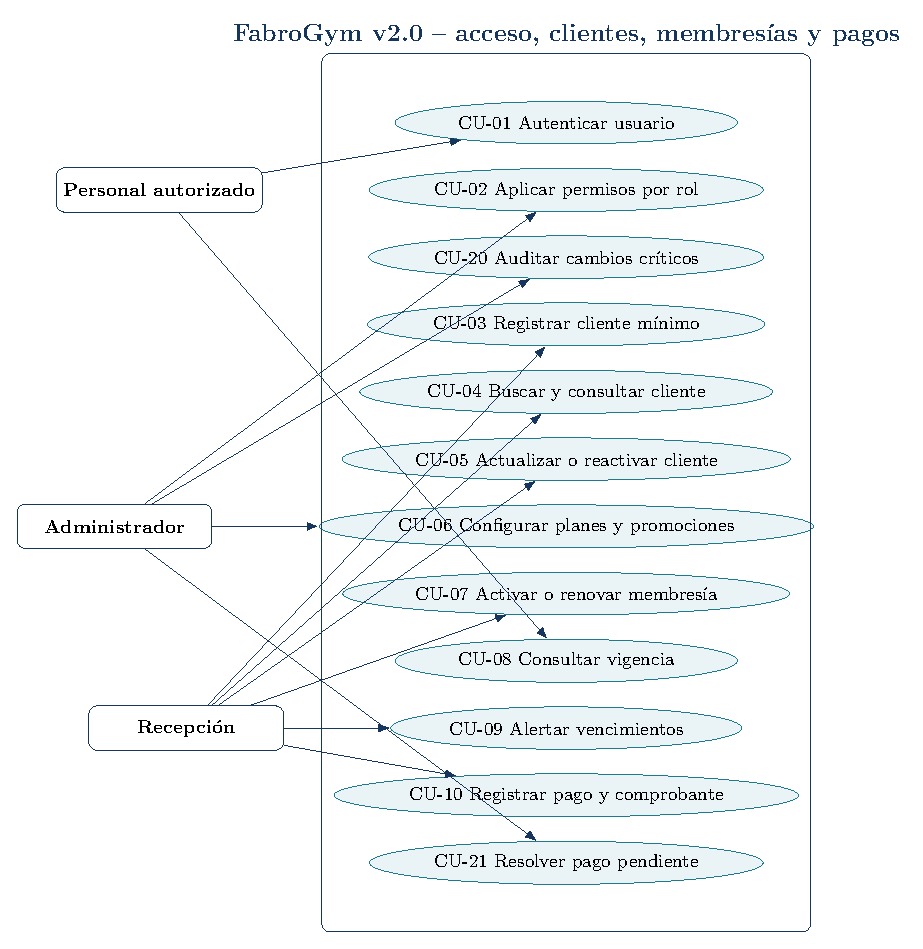
\includegraphics[width=.96\textwidth,height=.79\textheight,keepaspectratio]{casos_uso_v2_1.pdf}\caption{Casos de uso v2.0: acceso, clientes, membresías y pagos (CU-01 a CU-10, CU-20 y CU-21).}\end{figure}
\begin{figure}[H]\centering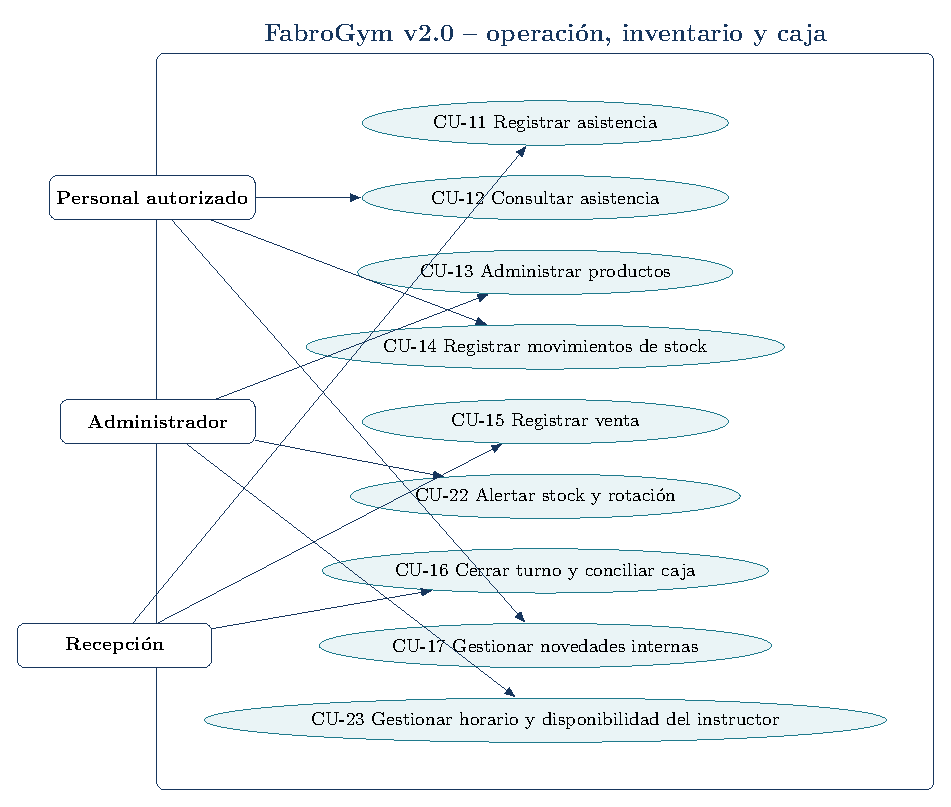
\includegraphics[width=.96\textwidth,height=.77\textheight,keepaspectratio]{casos_uso_v2_2.pdf}\caption{Casos de uso v2.0: asistencia, inventario, ventas, caja y operación (CU-11 a CU-17, CU-22 y CU-23).}\end{figure}
\begin{figure}[H]\centering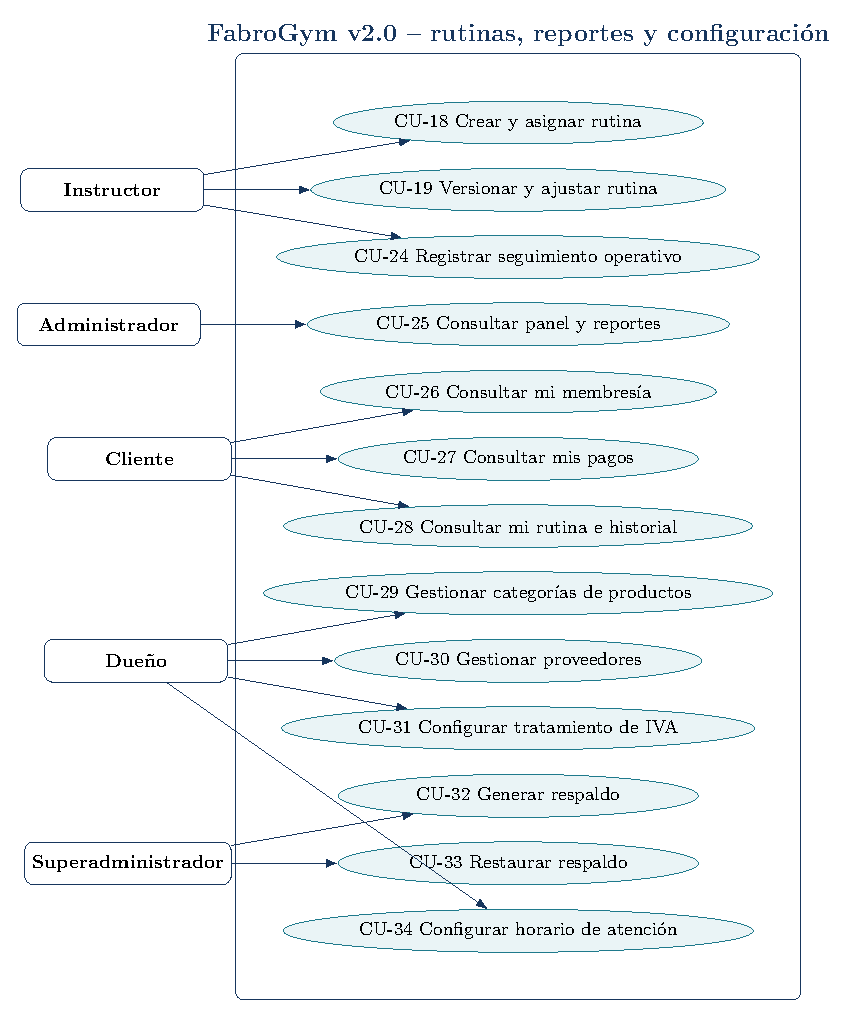
\includegraphics[width=.96\textwidth,height=.79\textheight,keepaspectratio]{casos_uso_v2_3.pdf}\caption{Casos de uso v2.0: rutinas, reportes, autoservicio, respaldo y configuración (CU-18, CU-19 y CU-24 a CU-34).}\end{figure}
\begin{figure}[H]\centering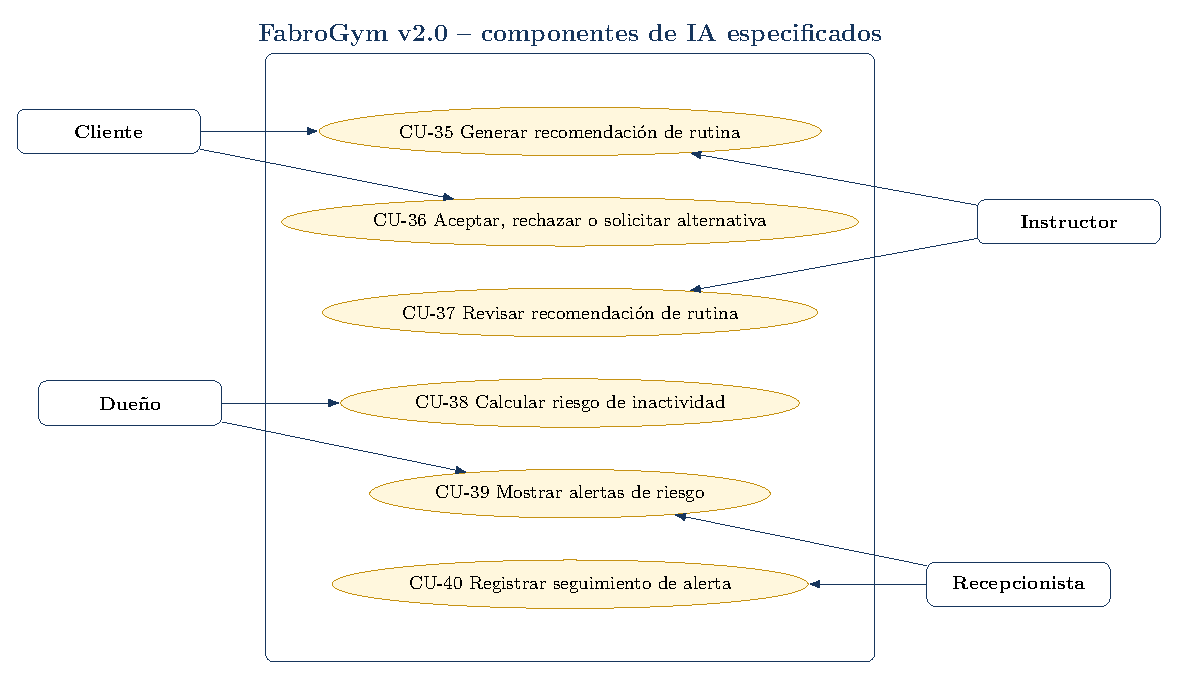
\includegraphics[width=.96\textwidth,height=.61\textheight,keepaspectratio]{casos_uso_v2_4_ia.pdf}\caption{Casos de uso v2.0 correspondientes a los componentes de IA especificados (CU-35 a CU-40).}\end{figure}

La primera vista concentra autenticación, autorización, clientes, membresías y pagos; la segunda reúne la operación diaria; la tercera presenta rutinas, reportes, autoservicio y configuración; y la cuarta separa los componentes de IA para hacer visible su carácter futuro y supervisado. Esta organización elimina la contradicción que existía entre el diagrama de entrada y el catálogo v2.0, especialmente para los CU-20 a CU-40.

\subsection{Especificación textual de los casos de uso}
La línea base identifica 40 casos de uso y los 40 se especifican mediante actor, precondición y escenario observable. Esta relación permite calcular M1b sin confundir un caso dibujado con un caso efectivamente especificado.

\begin{landscape}
\scriptsize
\begin{longtable}{|p{1.2cm}|p{1.9cm}|p{2.4cm}|p{5.0cm}|p{9.2cm}|}
\caption{Especificación textual resumida de CU-01 a CU-40.}\\
\hline\textbf{CU} & \textbf{RF} & \textbf{Actor} & \textbf{Precondición} & \textbf{Escenario principal / resultado observable}\\\hline
\endfirsthead
\hline\textbf{CU} & \textbf{RF} & \textbf{Actor} & \textbf{Precondición} & \textbf{Escenario principal / resultado observable}\\\hline
\endhead
CU-01 & RF-AUT-01 & Personal autorizado & Usuario registrado con credenciales activas. & Dado un usuario con credenciales válidas, cuando inicie sesión, entonces el sistema deberá autenticarlo y habilitar únicamente las opciones permitidas para su rol; cuando cierre sesión, deberá invalidar la sesión activa. \\ \hline
CU-02 & RF-AUT-02 & Administrador & Usuario autenticado y autorizado para el caso de uso. & Dado un usuario autenticado con un rol definido, cuando intente ejecutar una operación, entonces el sistema deberá permitirla solo si el permiso está asignado a ese rol y deberá denegarla en caso contrario. \\ \hline
CU-20 & RF-AUT-03 & Administrador & Usuario autenticado y autorizado para el caso de uso. & Dado un cambio crítico confirmado, cuando el sistema lo registre, entonces deberá conservar en auditoría el actor, fecha, acción, valor anterior y valor nuevo asociados al cambio. \\ \hline
CU-03 & RF-CLI-01 & Recepcionista & Usuario autenticado y autorizado para el caso de uso. & Dado un formulario con código interno, nombre de uso y al menos un medio de contacto válido, cuando Recepción confirme el registro, entonces el sistema deberá crear un único cliente y no deberá solicitar datos de salud, biometría, dirección domiciliaria ni imagen corporal. \\ \hline
CU-04 & RF-CLI-02 & Recepcionista & Usuario autenticado y autorizado para el caso de uso. & Dado un criterio de búsqueda válido, cuando Recepción consulte un cliente, entonces el sistema deberá devolver las coincidencias y mostrar únicamente membresía, último pago, asistencia y novedades autorizadas por el rol. \\ \hline
CU-05 & RF-CLI-03 & Recepcionista & Usuario autenticado y autorizado para el caso de uso. & Dado que existe un cliente coincidente por código o contacto, cuando Recepción intente registrar o reactivar el perfil, entonces el sistema deberá advertir la coincidencia y permitir actualizar o reactivar el registro existente sin crear un duplicado. \\ \hline
CU-06 & RF-MEM-01 & Administrador & Usuario autenticado y autorizado para el caso de uso. & Dado un usuario autorizado y los datos obligatorios de un plan o promoción, cuando guarde la configuración, entonces el sistema deberá conservar nombre, duración, precio, vigencia y estado y deberá mostrar el registro actualizado. \\ \hline
CU-07 & RF-MEM-02 & Recepcionista & Usuario autenticado y autorizado para el caso de uso. & Dado un plan vigente y un pago confirmado, cuando Recepción active o renueve la membresía, entonces el sistema deberá calcular y guardar las fechas de inicio y vencimiento según la duración del plan. \\ \hline
CU-08 & RF-MEM-03 & Personal autorizado & Usuario autenticado y autorizado para el caso de uso. & Dado un cliente con membresía registrada, cuando un usuario autorizado consulte su vigencia, entonces el sistema deberá mostrar estado, plan, fecha de inicio y fecha de vencimiento de la membresía seleccionada. \\ \hline
CU-09 & RF-MEM-04 & Recepcionista & Usuario autenticado y autorizado para el caso de uso. & Dado que existen membresías próximas a vencer o vencidas, cuando se ejecute la consulta diaria, entonces el sistema deberá separar las que vencen dentro de tres días de las ya vencidas y no deberá enviar mensajes externos de forma automática. \\ \hline
CU-10 & RF-PAG-01 & Recepcionista & Usuario autenticado y autorizado para el caso de uso. & Dado un pago con monto, concepto, medio, referencia y fecha válidos, cuando Recepción confirme el registro, entonces el sistema deberá guardar el pago y generar un comprobante interno vinculado al cliente. \\ \hline
CU-21 & RF-PAG-02 & Administrador & Usuario autenticado y autorizado para el caso de uso. & Dado un pago con estado pendiente, cuando un Administrador lo confirme, rechace o corrija, entonces el sistema deberá actualizar el estado y conservar el motivo y la evidencia de auditoría de la decisión. \\ \hline
CU-11 & RF-ASI-01 & Recepcionista & Usuario autenticado y autorizado para el caso de uso. & Dado un cliente identificado, cuando Recepción registre la asistencia por QR, entonces el sistema deberá guardar fecha, hora y método QR; si se utiliza contingencia manual, deberá exigir responsable y motivo. \\ \hline
CU-12 & RF-ASI-02 & Personal autorizado & Usuario autenticado y autorizado para el caso de uso. & Dado un filtro por cliente, fecha o turno, cuando un usuario autorizado consulte asistencias, entonces el sistema deberá mostrar únicamente los registros que cumplan el filtro y los conteos correspondientes. \\ \hline
CU-13 & RF-INV-01 & Administrador & Usuario autenticado y autorizado para el caso de uso. & Dado un producto con código, nombre, precio, unidad, stock mínimo y estado válidos, cuando el Administrador confirme el registro, entonces el sistema deberá guardar el producto y permitir su consulta posterior. \\ \hline
CU-14 & RF-INV-02 & Personal autorizado & Usuario autenticado y autorizado para el caso de uso. & Dado un producto existente y un movimiento válido, cuando un usuario autorizado registre una entrada o ajuste, entonces el sistema deberá actualizar el saldo y conservar cantidad, motivo, responsable y saldo resultante. \\ \hline
CU-15 & RF-VEN-01 & Recepcionista & Usuario autenticado y autorizado para el caso de uso. & Dado que todos los ítems de una venta tienen stock suficiente, cuando Recepción confirme la venta, entonces el sistema deberá registrar la venta y descontar las existencias en una única transacción; si falla una operación, no deberá aplicar cambios parciales. \\ \hline
CU-22 & RF-INV-03 & Administrador & Usuario autenticado y autorizado para el caso de uso. & Dado un período de consulta, cuando el Administrador solicite el control de stock, entonces el sistema deberá listar los productos con stock igual o inferior al mínimo y resumir entradas, salidas y ventas del período. \\ \hline
CU-16 & RF-CAJ-01 & Recepcionista & Usuario autenticado y autorizado para el caso de uso. & Dado un turno con pagos y ventas registrados, cuando Recepción ejecute el cierre, entonces el sistema deberá totalizar por medio de pago, comparar contra los valores declarados y registrar cualquier diferencia junto con la entrega del turno. \\ \hline
CU-17 & RF-NOV-01 & Personal autorizado & Usuario autenticado y autorizado para el caso de uso. & Dado un usuario autorizado y una novedad con categoría, detalle, responsable y vencimiento, cuando la registre, entonces el sistema deberá crearla con un estado válido y conservar los cambios posteriores de estado. \\ \hline
CU-23 & RF-INS-01 & Administrador & Usuario autenticado y autorizado para el caso de uso. & Dado un instructor registrado, cuando el Administrador actualice su operación, entonces el sistema deberá guardar turnos, capacidad, disponibilidad y novedades operativas sin solicitar datos de salud. \\ \hline
CU-18 & RF-RUT-01 & Instructor & Usuario autenticado y autorizado para el caso de uso. & Dado un cliente autorizado y un catálogo de ejercicios disponible, cuando el Instructor cree una rutina, entonces el sistema deberá guardar objetivo operativo, ejercicios, series, repeticiones, descanso y días, y deberá asignarla al cliente seleccionado. \\ \hline
CU-19 & RF-RUT-02 & Instructor & Usuario autenticado y autorizado para el caso de uso. & Dado una rutina existente, cuando el Instructor modifique ejercicios o parámetros y confirme el cambio, entonces el sistema deberá crear una nueva versión y mantener las versiones anteriores en solo lectura. \\ \hline
CU-24 & RF-RUT-03 & Instructor & Usuario autenticado y autorizado para el caso de uso. & Dado una rutina activa, cuando el Instructor registre seguimiento, entonces el sistema deberá guardar fecha, cumplimiento, repeticiones y observación operativa y deberá rechazar campos destinados a diagnósticos, lesiones, peso o medidas corporales reales. \\ \hline
CU-25 & RF-REP-01 & Administrador & Usuario autenticado y autorizado para el caso de uso. & Dado un período y filtros válidos, cuando el Administrador consulte el panel o reporte, entonces el sistema deberá calcular los indicadores con datos almacenados, mostrar los resultados filtrados y permitir exportarlos a CSV. \\ \hline
CU-26 & RF-MEM-05 & Cliente & Usuario autenticado y autorizado para el caso de uso. & Dado un Cliente autenticado, cuando consulte su membresía, entonces el sistema deberá mostrar únicamente el estado, plan y vigencia de su propia membresía y no deberá habilitar edición. \\ \hline
CU-27 & RF-PAG-03 & Cliente & Usuario autenticado y autorizado para el caso de uso. & Dado un Cliente autenticado, cuando consulte sus pagos, entonces el sistema deberá mostrar únicamente sus registros de pago y el estado de cada uno en modo de solo lectura. \\ \hline
CU-28 & RF-RUT-04 & Cliente & Usuario autenticado y autorizado para el caso de uso. & Dado un Cliente autenticado con una rutina asignada, cuando consulte su rutina, entonces el sistema deberá mostrar la versión activa, las versiones históricas y el seguimiento autorizado sin permitir modificar la rutina vigente. \\ \hline
CU-29 & RF-INV-04 & Dueño & Usuario autenticado y autorizado para el caso de uso. & Dado un usuario autorizado, cuando registre, edite o desactive una categoría, entonces el sistema deberá guardar el cambio y reflejar el estado actualizado en las consultas de categorías. \\ \hline
CU-30 & RF-INV-05 & Dueño & Usuario autenticado y autorizado para el caso de uso. & Dado un usuario autorizado, cuando registre, edite o desactive un proveedor, entonces el sistema deberá guardar el cambio y reflejar el estado actualizado en las consultas de proveedores. \\ \hline
CU-31 & RF-CFG-01 & Dueño & Usuario autenticado y autorizado para el caso de uso. & Dado un porcentaje de IVA válido y la configuración tributaria de un producto, cuando el Dueño confirme el cambio, entonces el sistema deberá aplicar la nueva configuración a operaciones posteriores y conservar el valor anterior, el nuevo valor, el actor y la fecha. \\ \hline
CU-32 & RF-BCK-01 & Superadministrador & Superadministrador autenticado y almacenamiento de respaldo disponible. & Dado un Superadministrador autenticado, cuando solicite un respaldo, entonces el sistema deberá iniciar el proceso cifrado, asignar un identificador y mostrar el estado y la fecha de finalización cuando concluya. \\ \hline
CU-33 & RF-BCK-02 & Superadministrador & Superadministrador autenticado y almacenamiento de respaldo disponible. & Dado un respaldo íntegro seleccionado, cuando el Superadministrador confirme explícitamente la restauración, entonces el sistema deberá verificar su integridad, ejecutar la restauración y registrar la operación en auditoría; si la verificación falla, no deberá restaurar. \\ \hline
CU-34 & RF-CFG-02 & Dueño & Usuario autenticado y autorizado para el caso de uso. & Dado un Dueño autenticado y una configuración válida de días y horas, cuando guarde el horario, entonces el sistema deberá actualizarlo y mostrar al Cliente únicamente el horario vigente. \\ \hline
CU-35 & RF-IA-RUT-01 & Cliente/Instructor & Actor autenticado; datos de entrada disponibles; componente de IA habilitado para evaluación. & Dado un objetivo operativo, disponibilidad semanal, historial no sensible y catálogo autorizado, cuando se solicite una recomendación, entonces el componente deberá devolver como máximo tres alternativas ordenadas de rutina y una explicación de los factores utilizados. \\ \hline
CU-36 & RF-IA-RUT-02 & Cliente & Actor autenticado; datos de entrada disponibles; componente de IA habilitado para evaluación. & Dado que el Cliente visualiza una recomendación de rutina, cuando seleccione aceptar, rechazar o solicitar alternativa, entonces el sistema deberá registrar la decisión y no deberá activar automáticamente la recomendación. \\ \hline
CU-37 & RF-IA-RUT-03 & Instructor & Actor autenticado; datos de entrada disponibles; componente de IA habilitado para evaluación. & Dado una recomendación aceptada por el Cliente, cuando el Instructor la revise, entonces el sistema deberá permitir aprobarla o rechazarla con motivo; únicamente una aprobación explícita podrá habilitar su activación. \\ \hline
CU-38 & RF-IA-ABA-01 & Dueño & Actor autenticado; datos de entrada disponibles; componente de IA habilitado para evaluación. & Dado el historial de asistencia, vigencia de membresía y frecuencia histórica de un cliente, cuando se ejecute el cálculo semanal, entonces el componente deberá asignar un nivel bajo, medio o alto y registrar la fecha del cálculo. \\ \hline
CU-39 & RF-IA-ABA-02 & Dueño/Recepcionista & Actor autenticado; datos de entrada disponibles; componente de IA habilitado para evaluación. & Dado que existen clientes clasificados con riesgo medio o alto, cuando Dueño o Recepcionista consulte las alertas, entonces el sistema deberá mostrar el nivel, la fecha y los principales factores de cada alerta sin ejecutar acciones automáticas. \\ \hline
CU-40 & RF-IA-ABA-03 & Recepcionista & Actor autenticado; datos de entrada disponibles; componente de IA habilitado para evaluación. & Dado una alerta de riesgo visible, cuando Recepción registre contacto, aplazamiento o descarte, entonces el sistema deberá guardar la acción, responsable, fecha y observación para auditoría. \\ \hline
\end{longtable}
\normalsize
\end{landscape}

\begin{figure}[H]\centering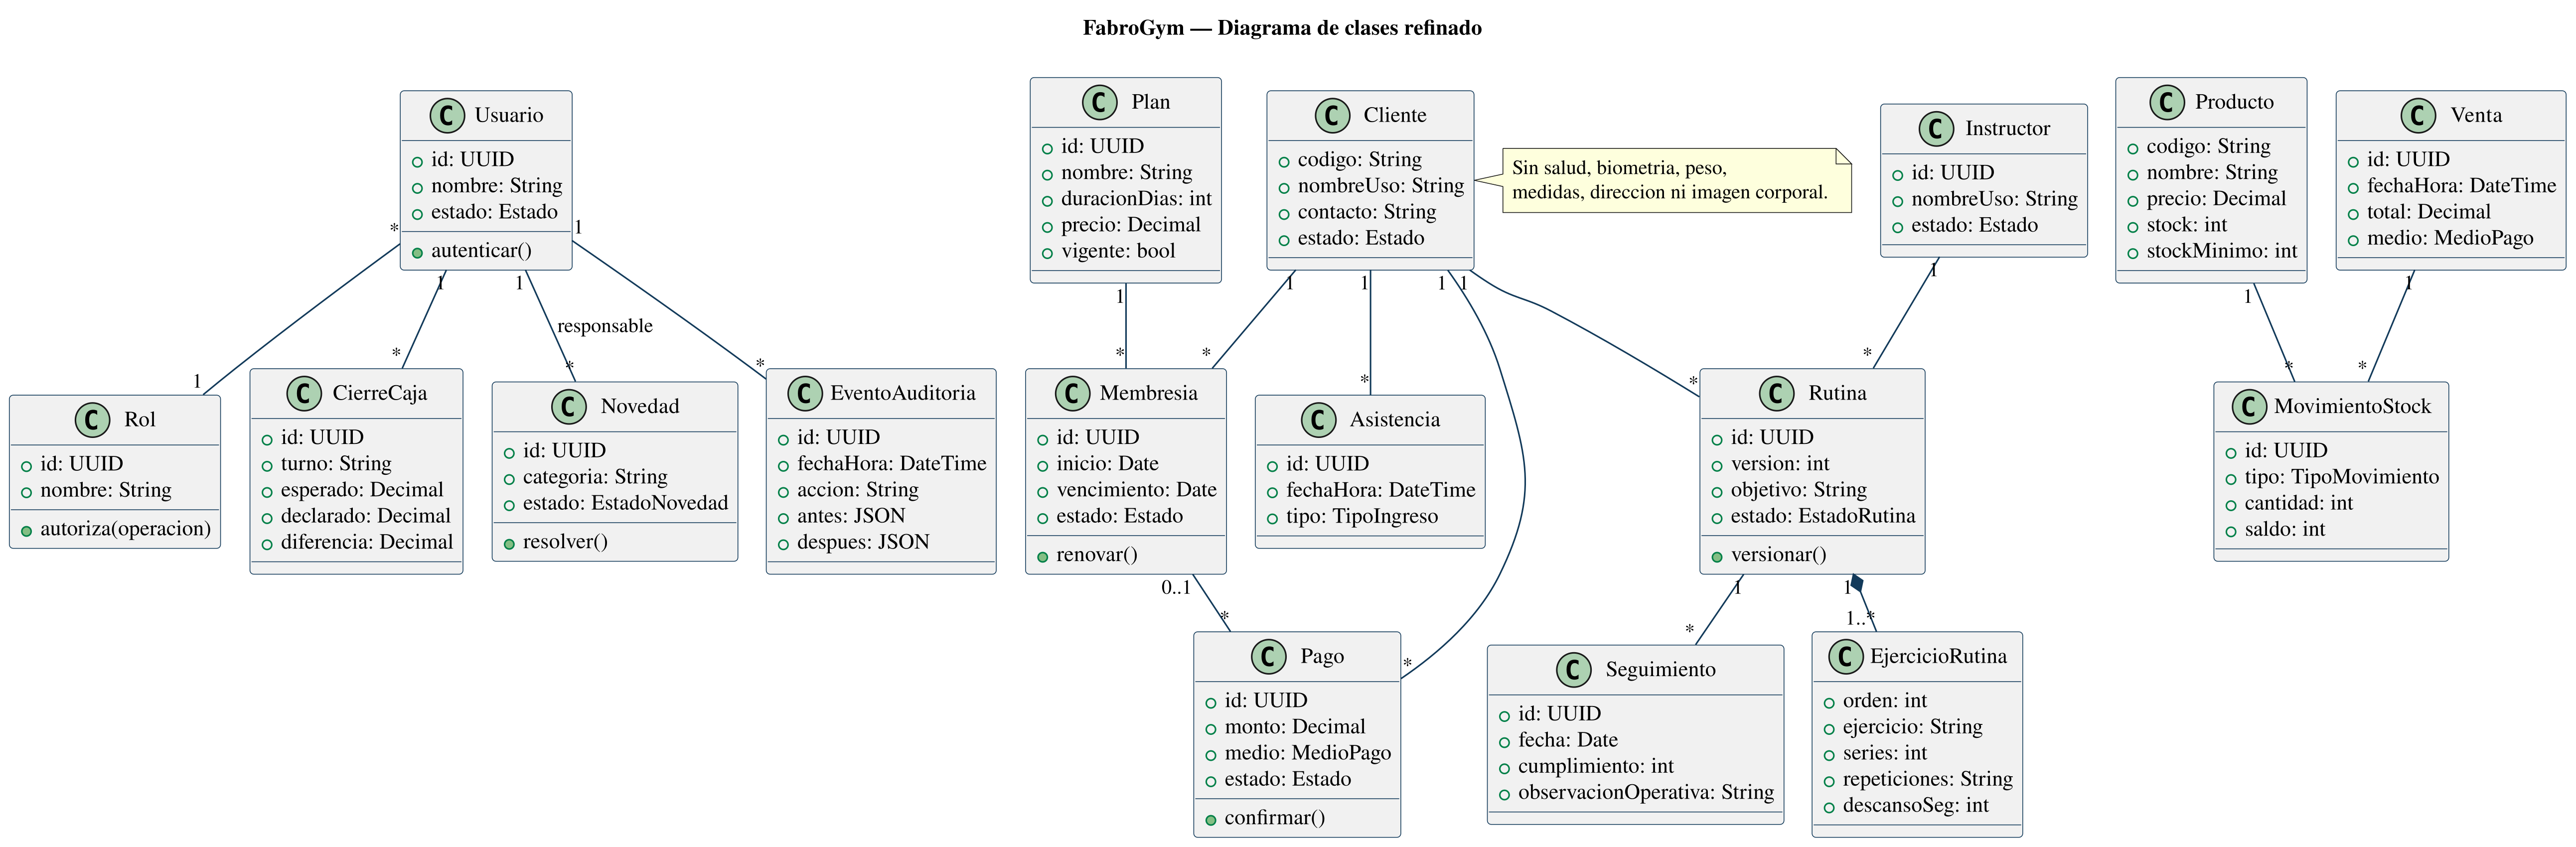
\includegraphics[width=.96\textwidth,height=.76\textheight,keepaspectratio]{clases.png}\caption{Modelo de clases disponible como base de dominio.}\end{figure}
\begin{figure}[H]\centering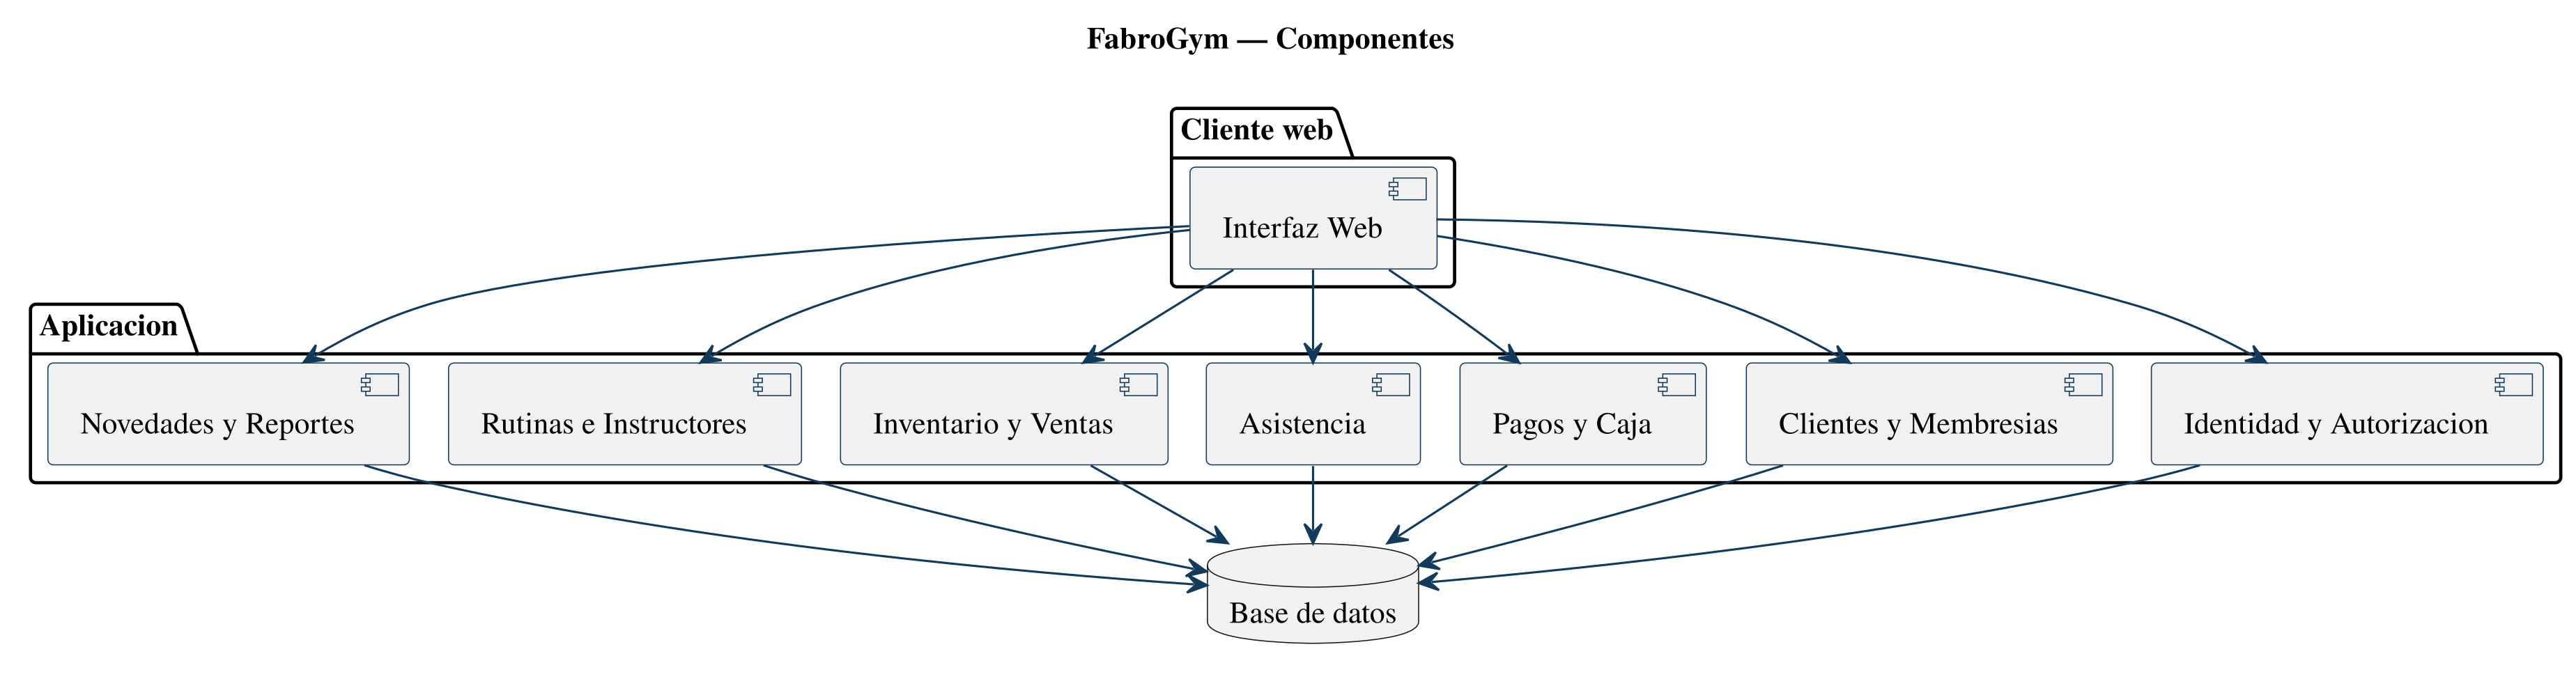
\includegraphics[width=.9\textwidth]{componentes.png}\caption{Vista de componentes de FabroGym.}\end{figure}
\begin{figure}[H]\centering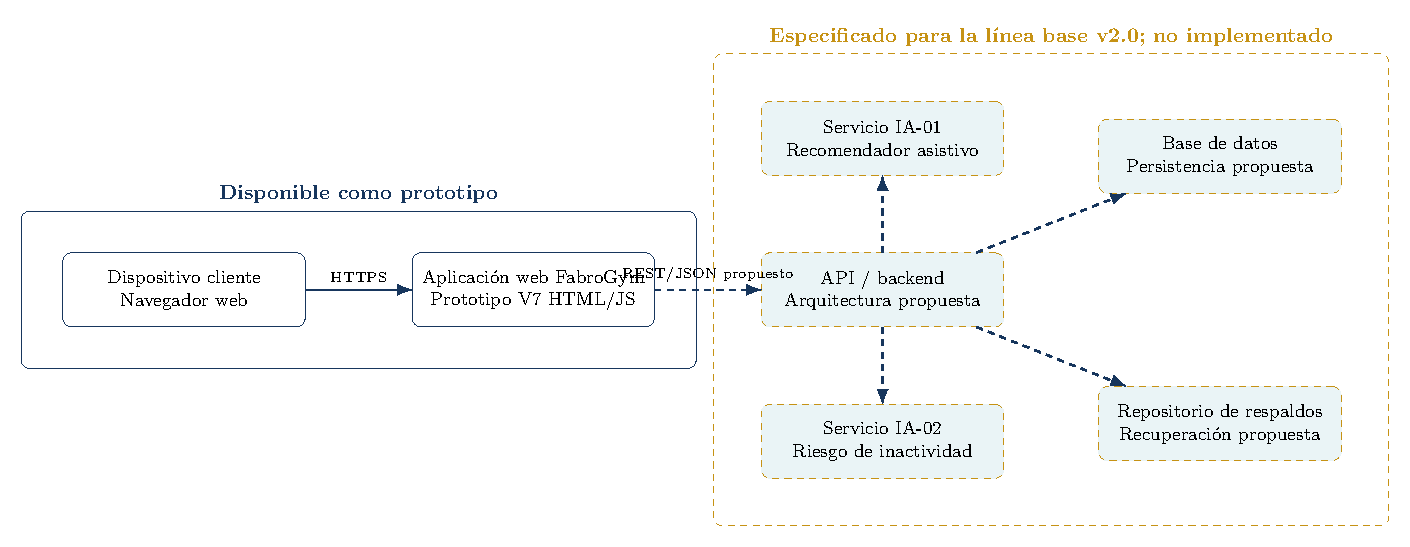
\includegraphics[width=.98\textwidth]{despliegue_v2_propuesto.pdf}\caption{Diagrama de despliegue v2.0: separación entre el prototipo disponible y la arquitectura propuesta.}\end{figure}

El despliegue distingue deliberadamente dos niveles de madurez. El navegador y la aplicación HTML/JavaScript corresponden al prototipo V7 disponible. La API, la persistencia, el repositorio de respaldo y los servicios IA-01/IA-02 representan nodos especificados para desarrollo posterior. Por tanto, el diagrama documenta la arquitectura objetivo sin convertirla en evidencia de ejecución.
\begin{figure}[H]\centering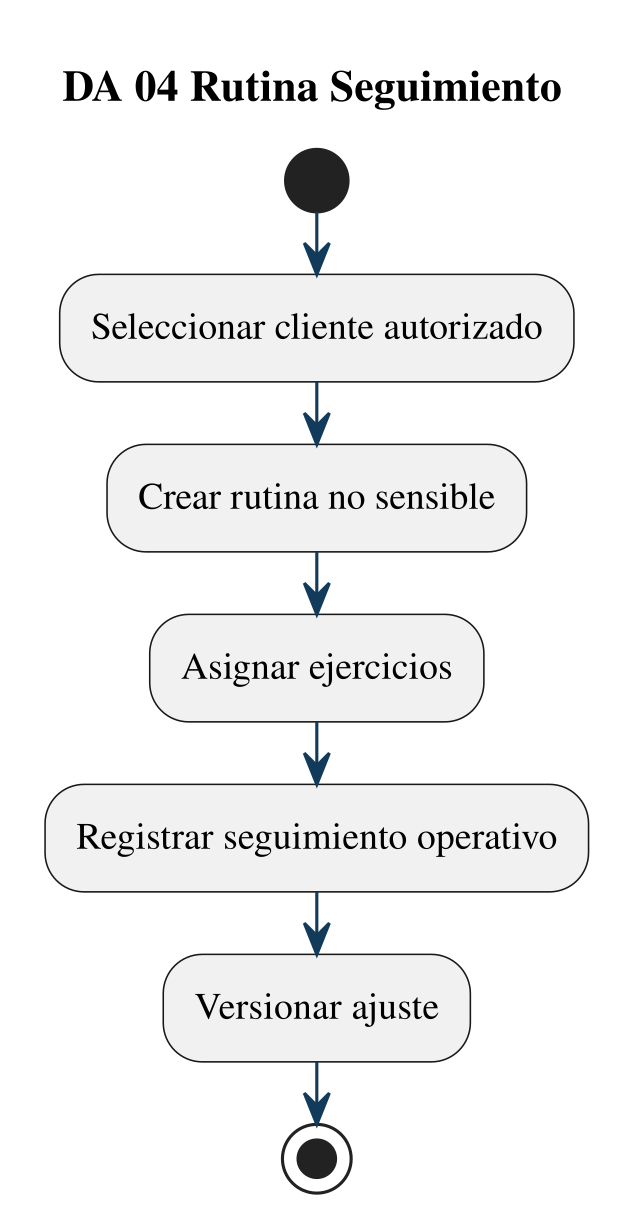
\includegraphics[width=.86\textwidth]{actividad_rutina.png}\caption{Actividad de rutina y seguimiento, relevante para IA-01.}\end{figure}



\subsection{Modelo funcional mediante DFD}
La matriz final utiliza procesos P-01 a P-15 como eslabón explícito de trazabilidad. Para que esa columna disponga también de una representación visual auditable, la PE5 incorpora un DFD de contexto y un DFD de nivel 1 regenerados desde la línea base final. El DFD no constituye evidencia de implementación: representa el movimiento lógico de información y diferencia mediante trazo discontinuo los procesos de respaldo e IA que permanecen especificados como arquitectura objetivo.
\begin{figure}[H]\centering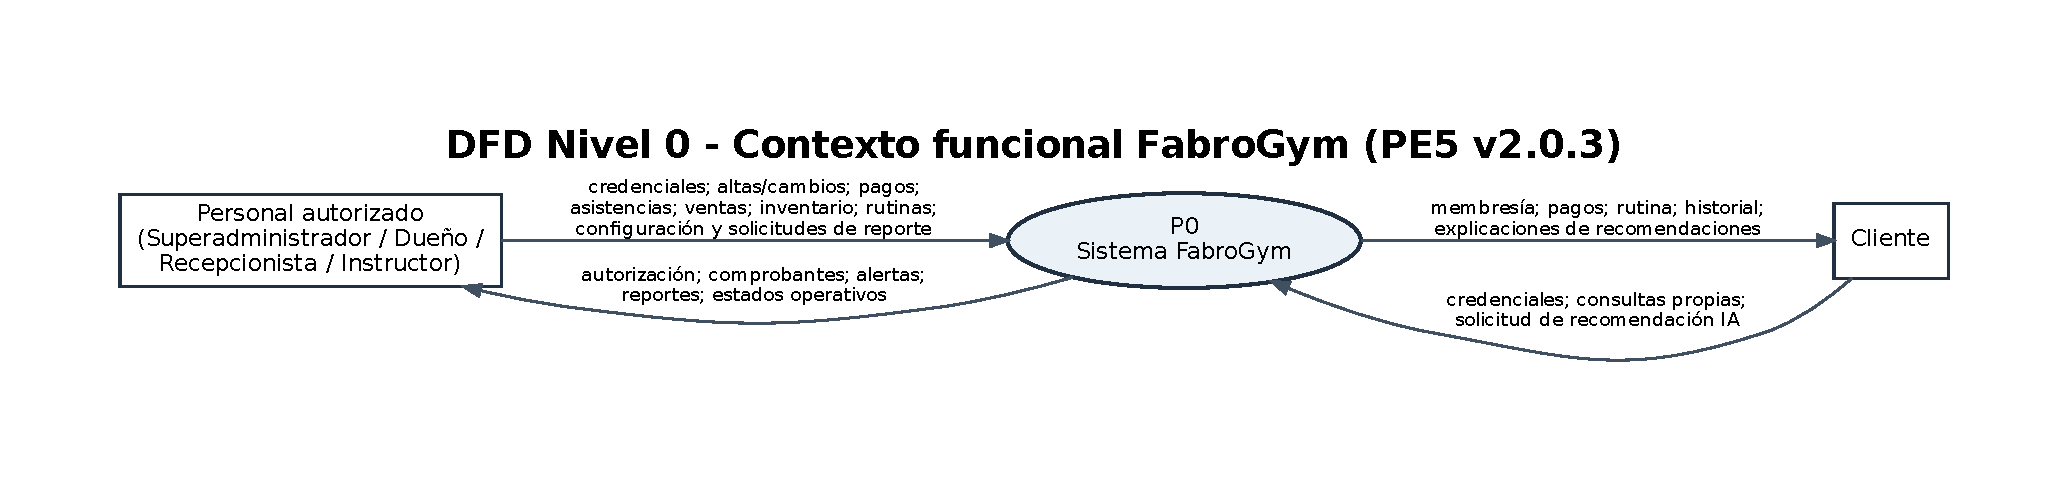
\includegraphics[width=.94\textwidth]{DFD_N0_FabroGym.pdf}\caption{DFD Nivel 0 de FabroGym: actores externos y frontera funcional del sistema.}\end{figure}
\begin{landscape}\begin{figure}[H]\centering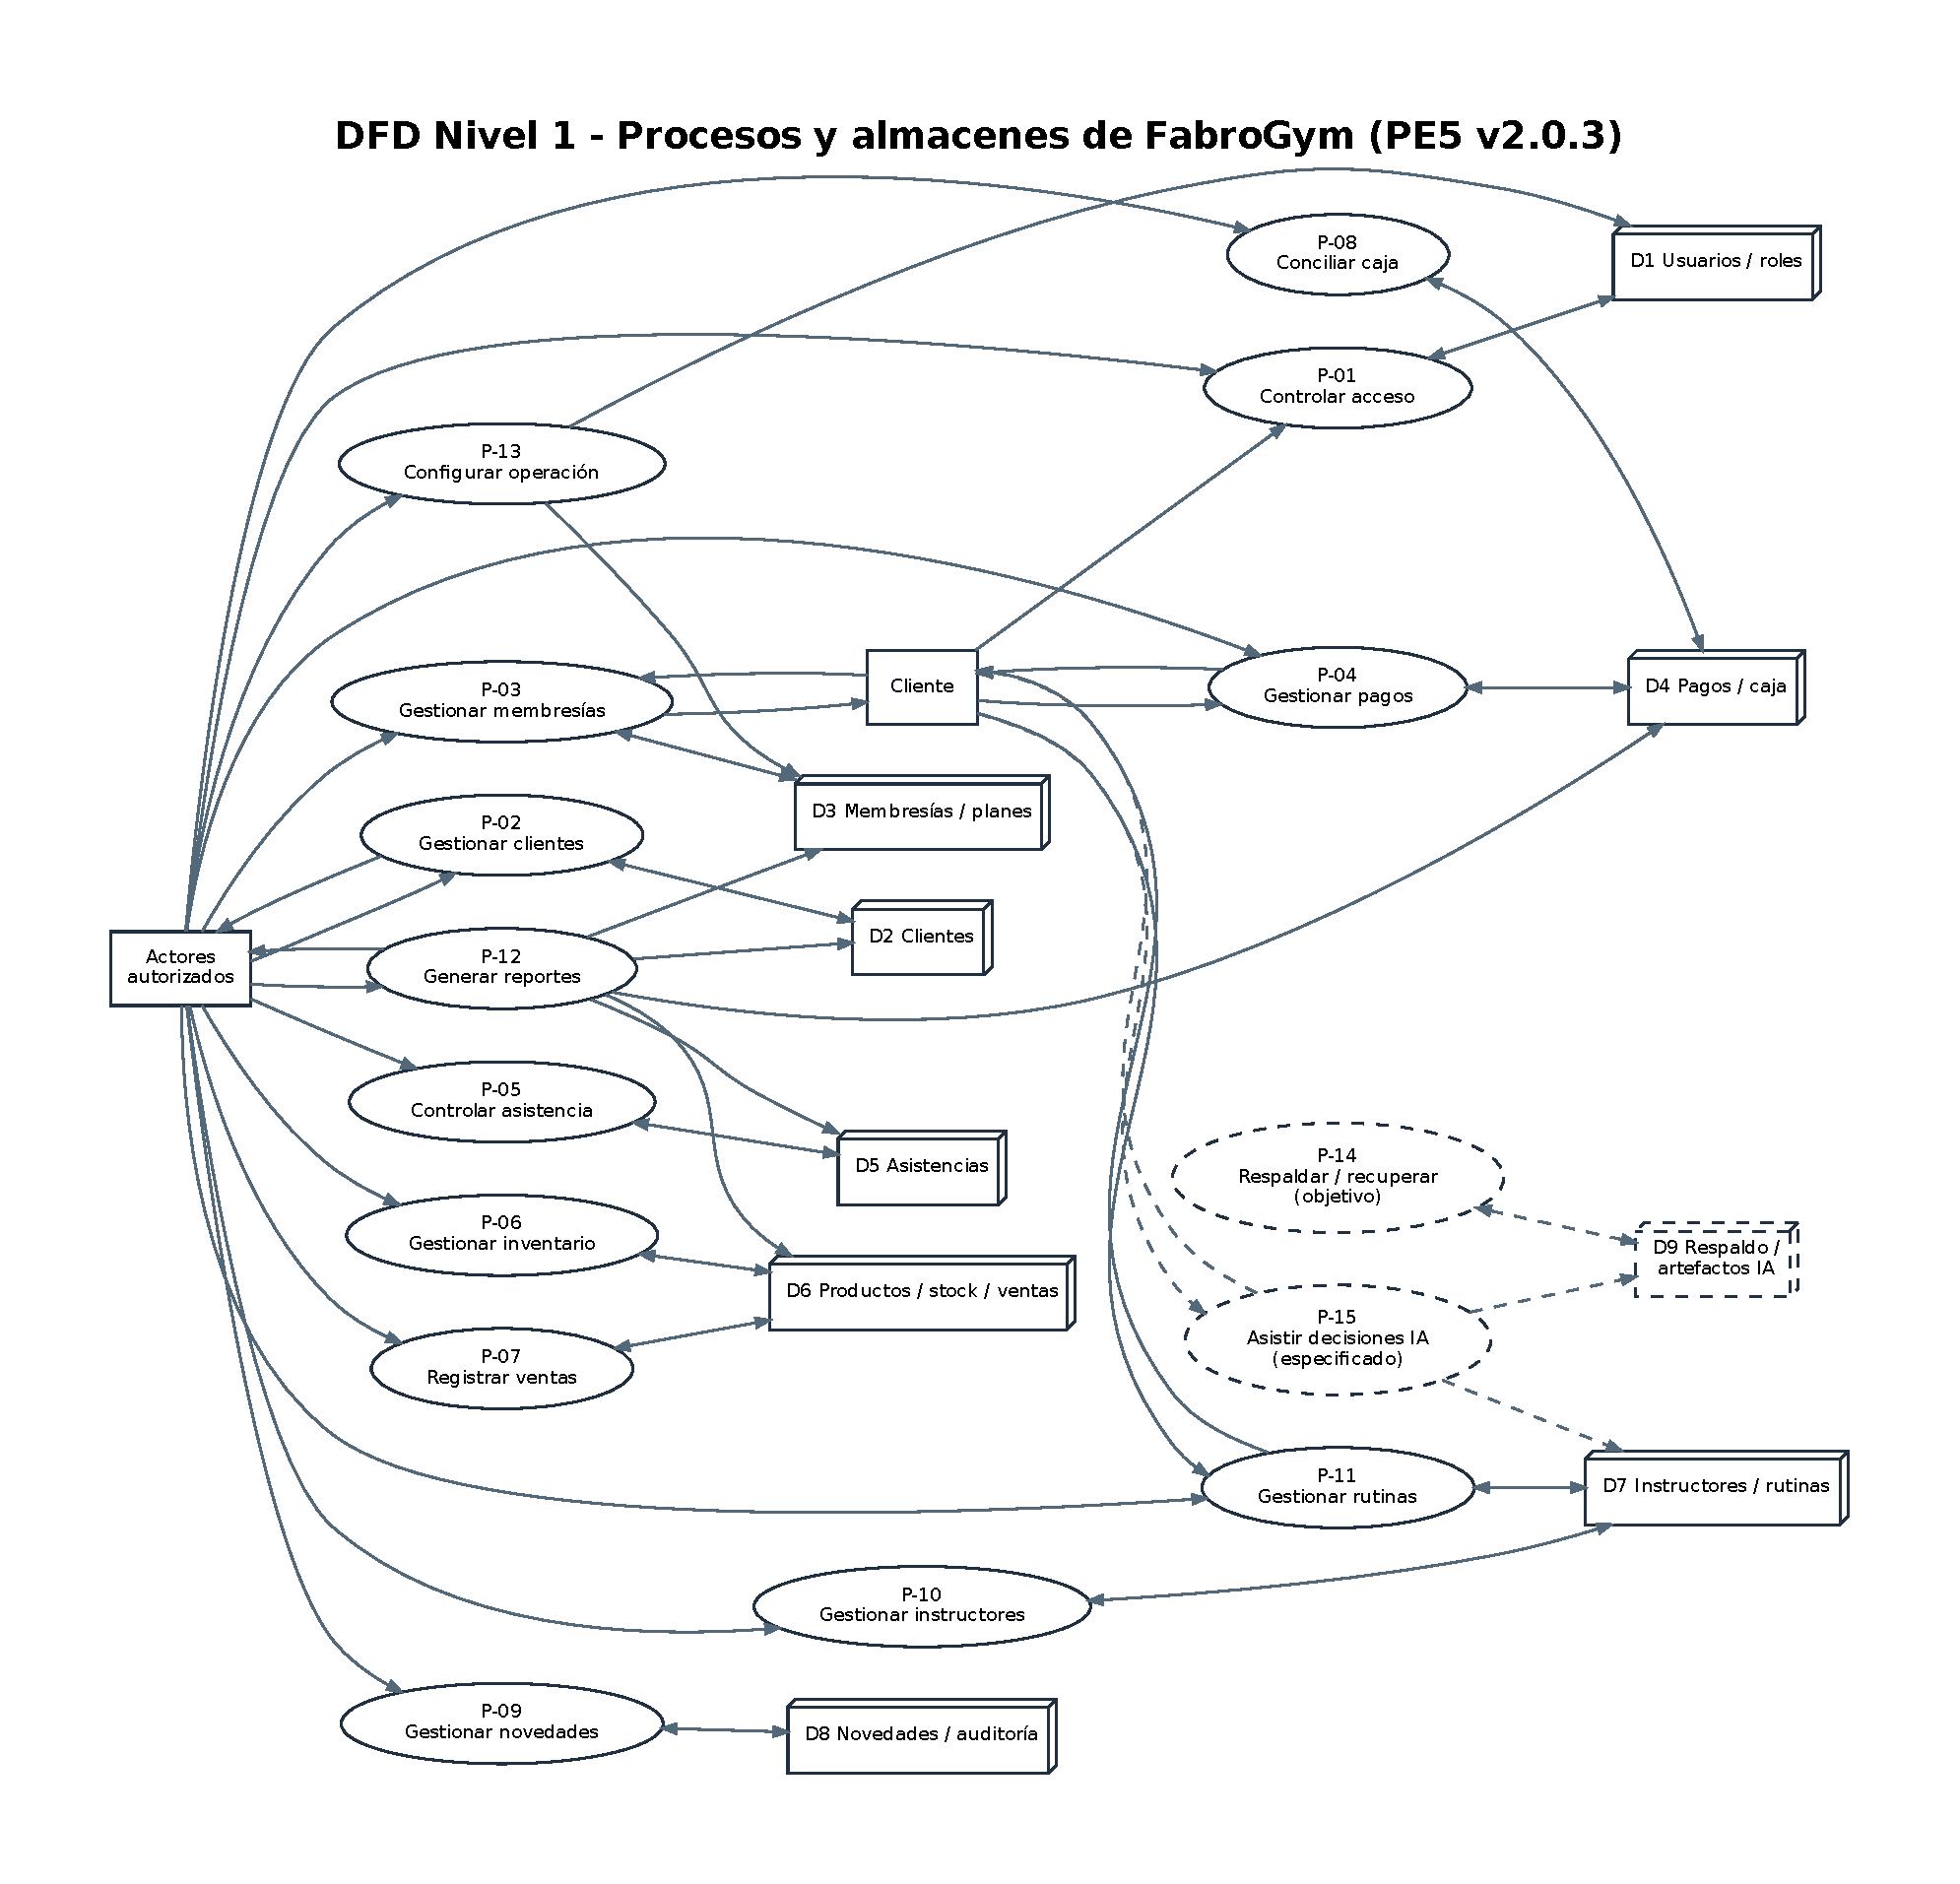
\includegraphics[width=.98\linewidth,height=.82\textheight,keepaspectratio]{DFD_N1_FabroGym.pdf}\caption{DFD Nivel 1 de FabroGym: procesos P-01 a P-15 y almacenes de datos relacionados con la matriz final.}\end{figure}\end{landscape}

\subsection{Máquinas de estados recuperadas y alineadas a la línea base final}
El PFC ya había modelado entidades con ciclo de vida no trivial en versiones anteriores. Para evitar que el paquete PE5 pierda esa perspectiva, se regeneran cuatro máquinas de estados coherentes con los requisitos y con la columna Estado/transición de la matriz: Membresía, Pago, Novedad y Rutina. La regeneración actualiza etiquetas y transiciones al catálogo v2.0 sin introducir nuevos requisitos.
\begin{figure}[H]\centering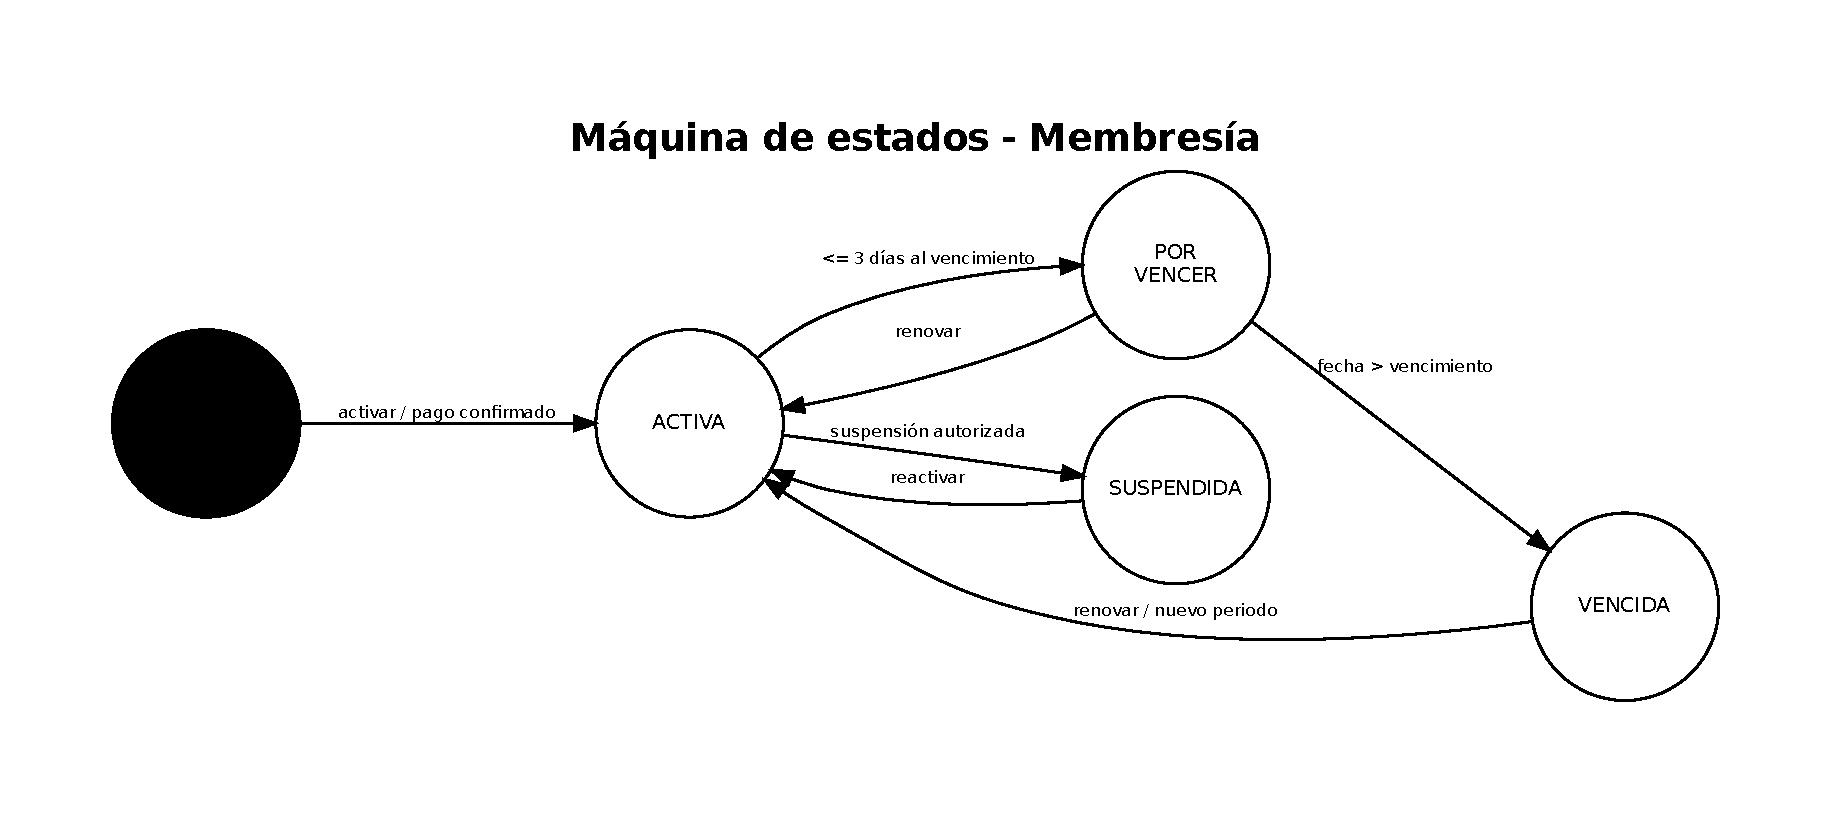
\includegraphics[width=.88\textwidth]{DE_01_Membresia_v2_0_3.pdf}\caption{Máquina de estados de Membresía alineada con RF-MEM-02, RF-MEM-03 y RF-MEM-04.}\end{figure}
\begin{figure}[H]\centering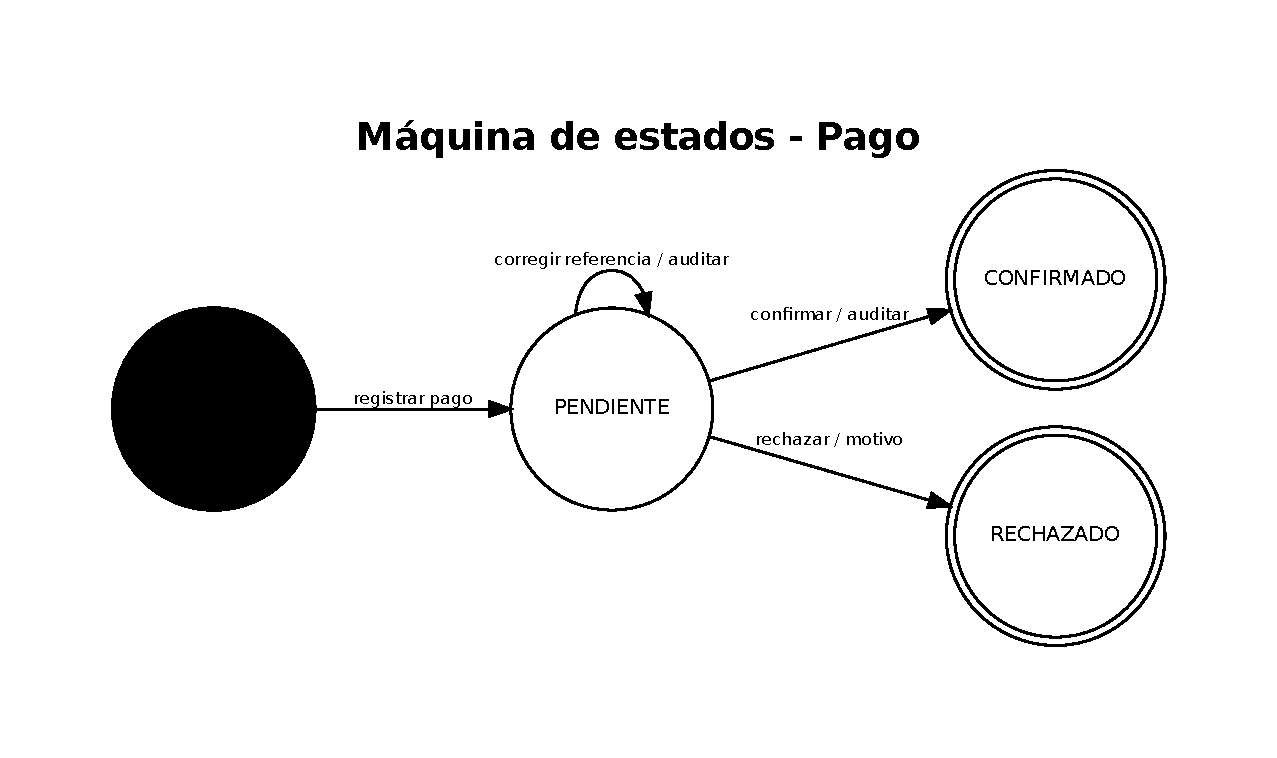
\includegraphics[width=.84\textwidth]{DE_02_Pago_v2_0_3.pdf}\caption{Máquina de estados de Pago alineada con RF-PAG-01 y RF-PAG-02.}\end{figure}
\begin{figure}[H]\centering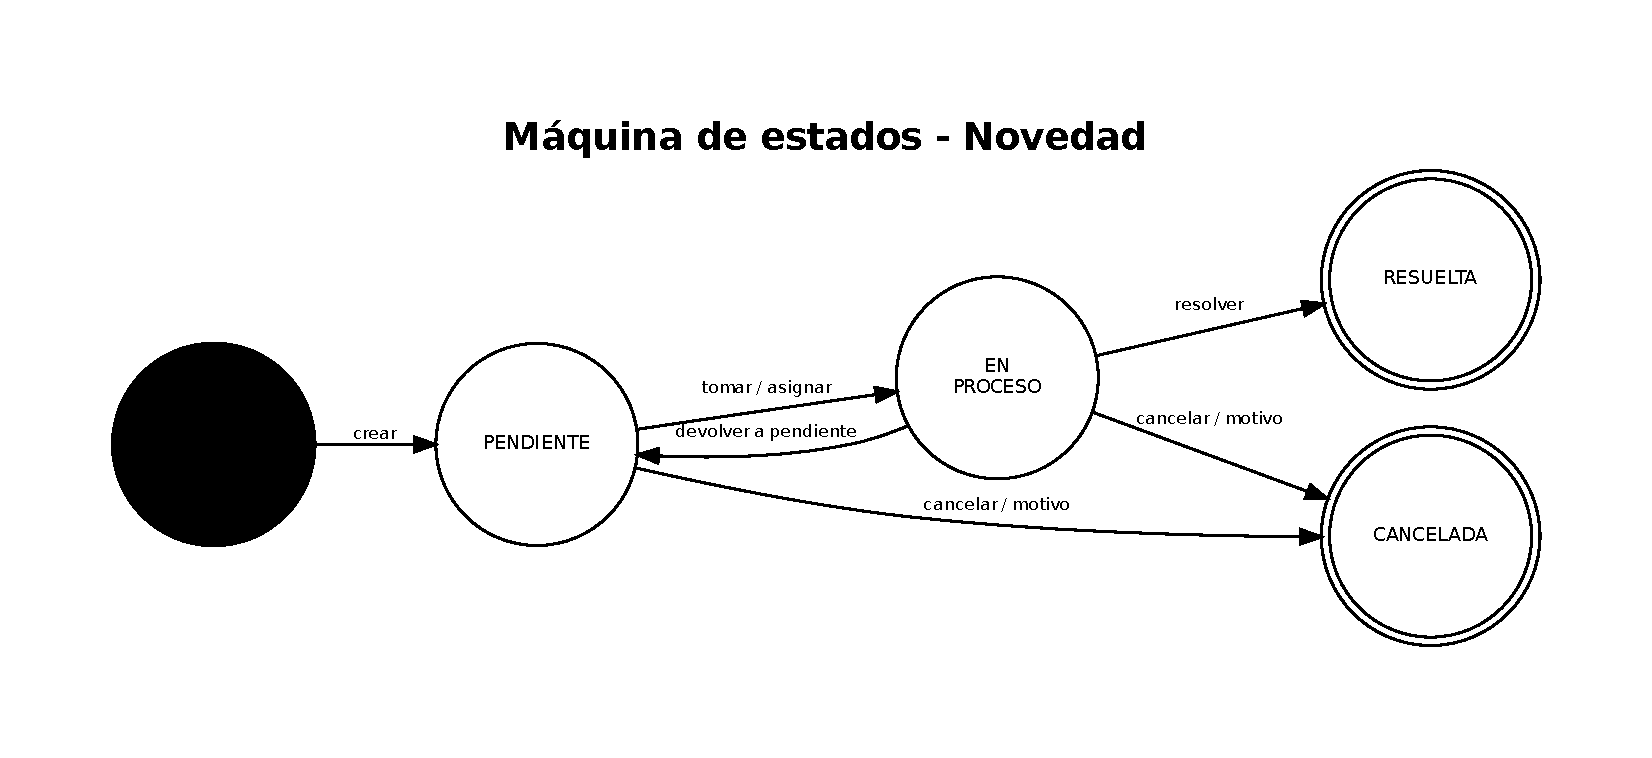
\includegraphics[width=.84\textwidth]{DE_03_Novedad_v2_0_3.pdf}\caption{Máquina de estados de Novedad alineada con RF-NOV-01.}\end{figure}
\begin{figure}[H]\centering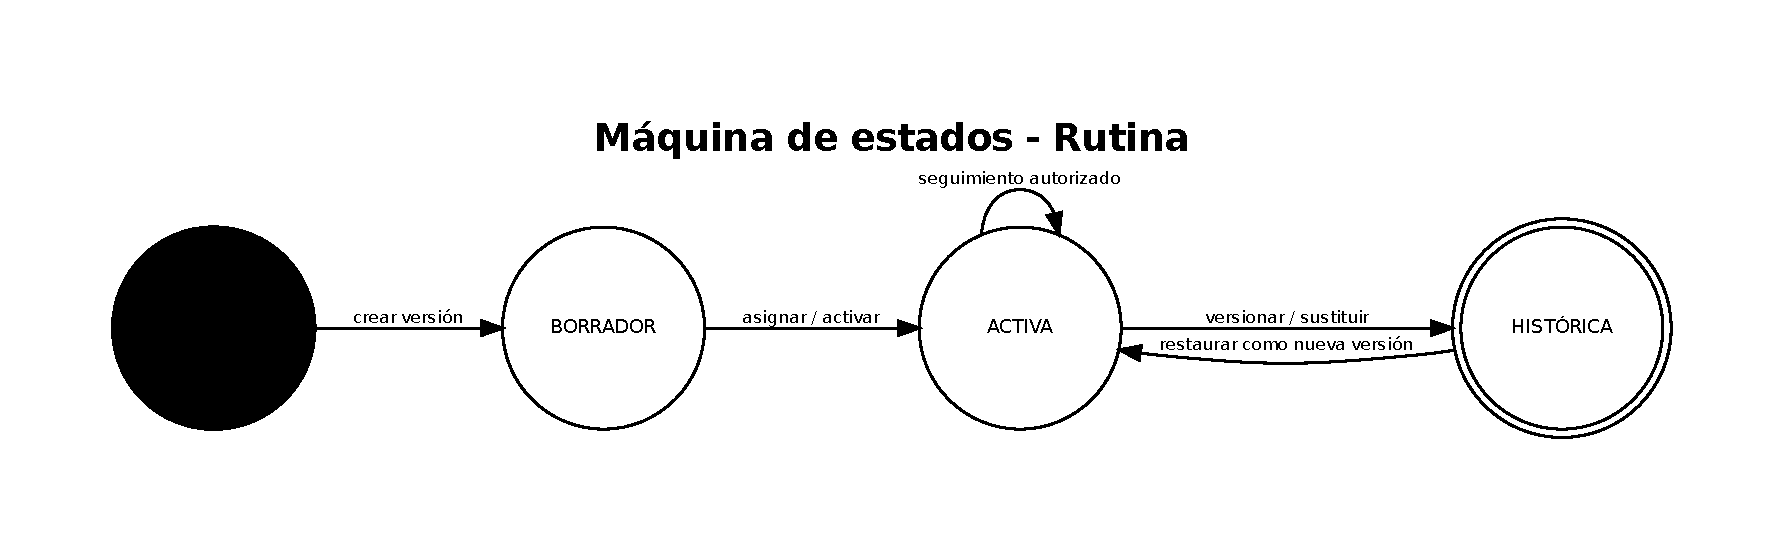
\includegraphics[width=.84\textwidth]{DE_04_Rutina_v2_0_3.pdf}\caption{Máquina de estados de Rutina alineada con RF-RUT-01, RF-RUT-02 y RF-RUT-04.}\end{figure}

\subsection{Secuencias representativas}
La línea base histórica de FabroGym ya contemplaba secuencias para requisitos Must. En PE5 se incorporan tres secuencias representativas actualizadas para autenticación, pagos y ventas, seleccionadas por cubrir seguridad, actualización de estado y consistencia transaccional. Son modelos conceptuales derivados de RF y BDD; no se presentan como traza de ejecución de un backend inexistente.
\begin{figure}[H]\centering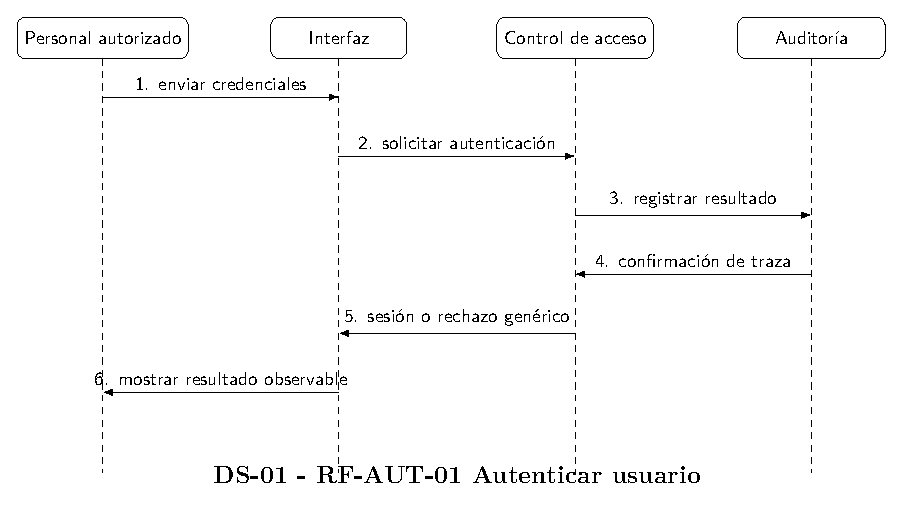
\includegraphics[width=.96\textwidth]{DS_01_RF-AUT-01_v2_0_3.pdf}\caption{Secuencia conceptual de RF-AUT-01: autenticar usuario.}\end{figure}
\begin{figure}[H]\centering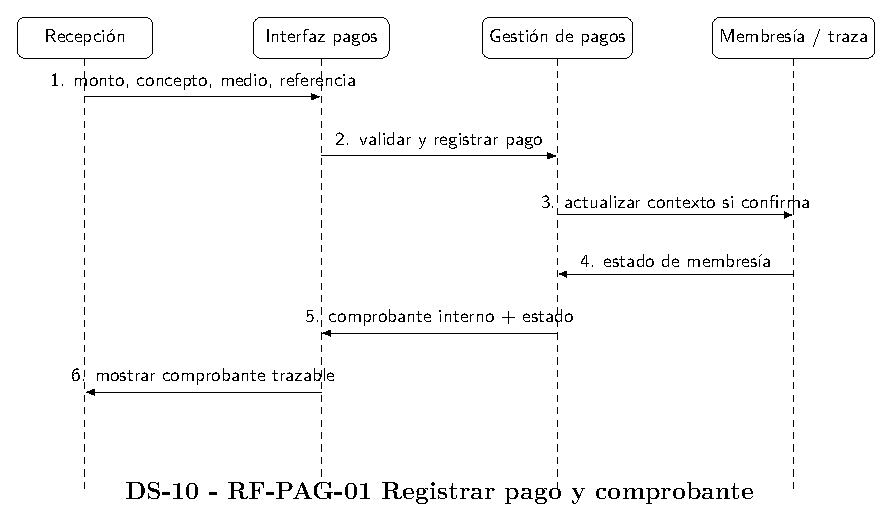
\includegraphics[width=.96\textwidth]{DS_10_RF-PAG-01_v2_0_3.pdf}\caption{Secuencia conceptual de RF-PAG-01: registrar pago y comprobante.}\end{figure}
\begin{figure}[H]\centering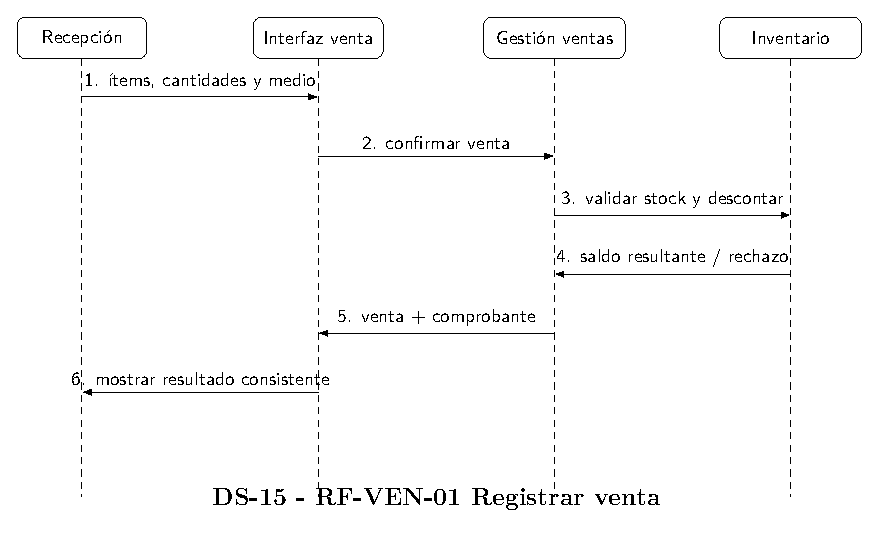
\includegraphics[width=.96\textwidth]{DS_15_RF-VEN-01_v2_0_3.pdf}\caption{Secuencia conceptual de RF-VEN-01: registrar venta y actualizar inventario.}\end{figure}

\subsection{Evidencia visual del prototipo V7}
Las pantallas siguientes demuestran cobertura visual y navegación del prototipo, no persistencia terminal. Su integración permite contrastar requisitos y modelos con la interfaz disponible, manteniendo la diferencia entre prototipado e implementación.
\begin{figure}[H]\centering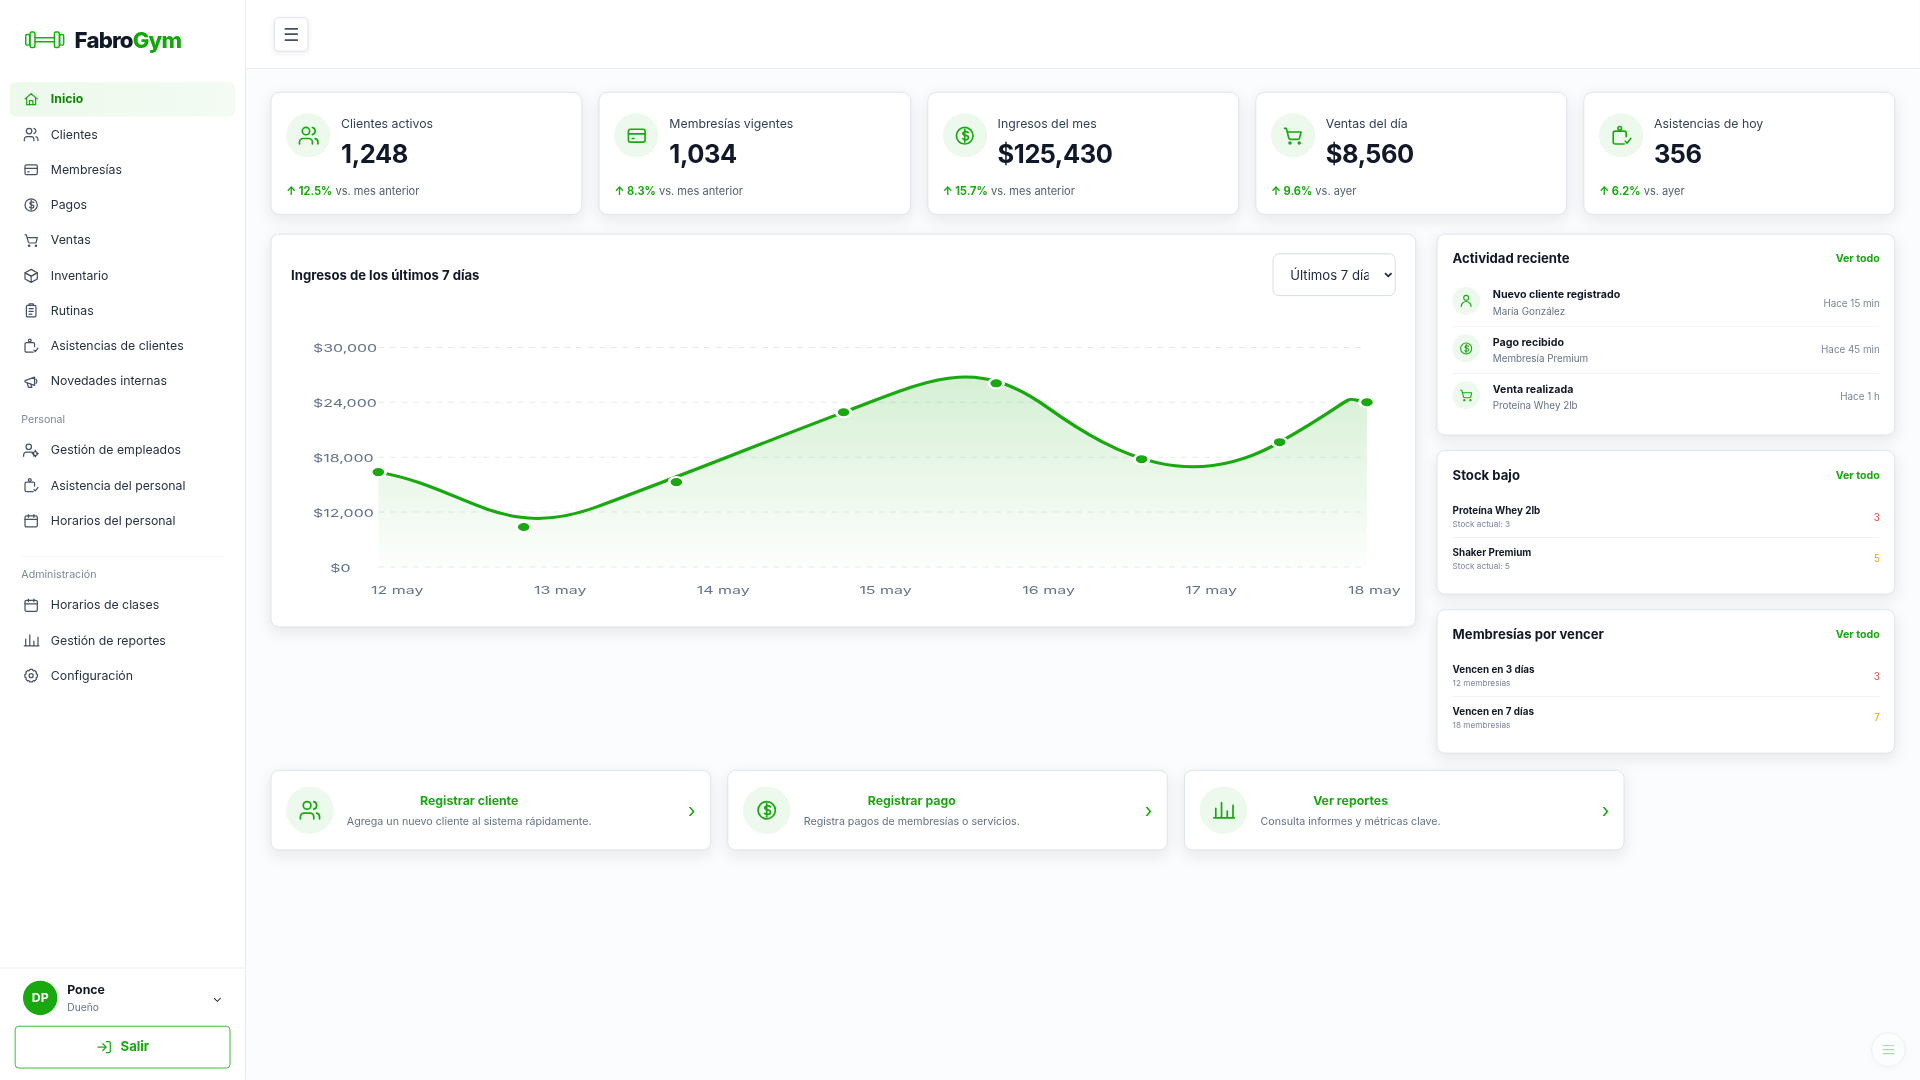
\includegraphics[width=.92\textwidth]{dashboard.png}\caption{Dashboard del prototipo V7 usado para contrastar paneles y reportes.}\end{figure}
\begin{figure}[H]\centering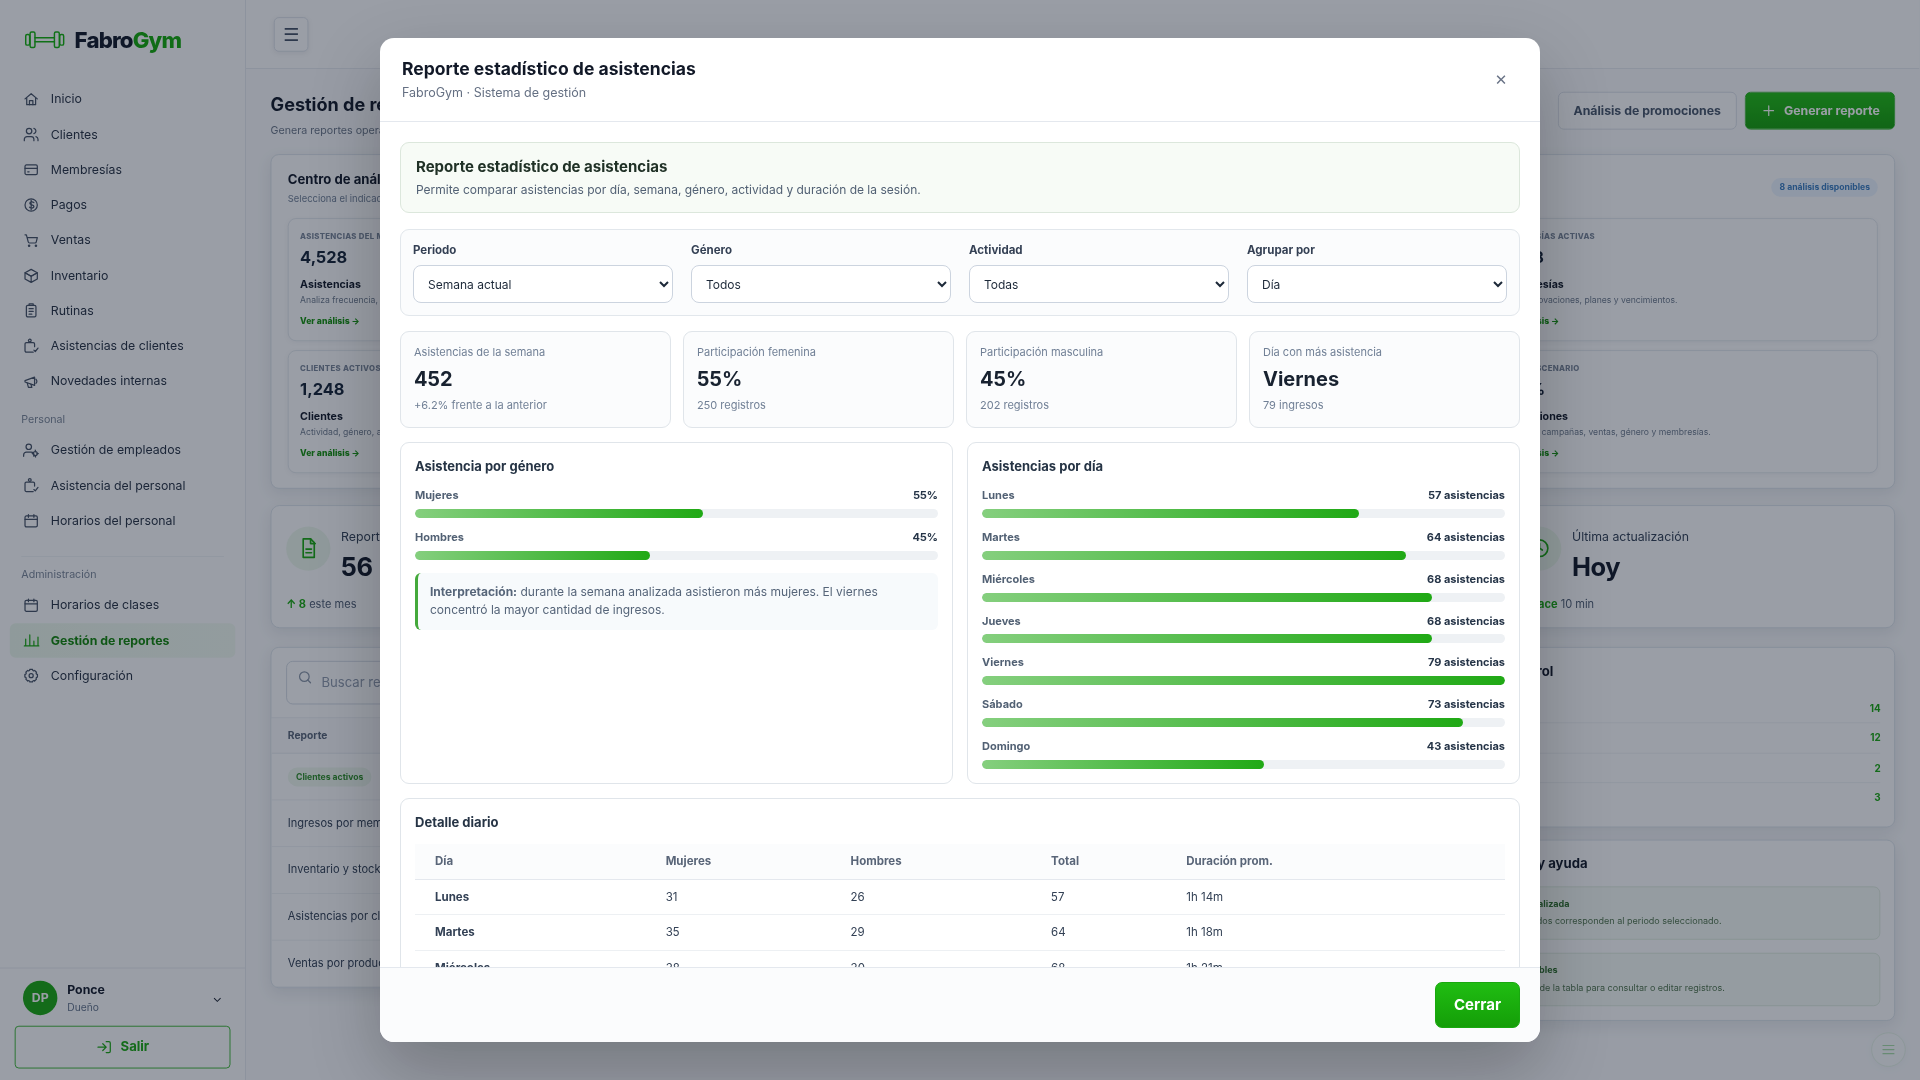
\includegraphics[width=.92\textwidth]{reporte_asistencia.png}\caption{Vista del reporte de asistencia del prototipo V7.}\end{figure}
\begin{figure}[H]\centering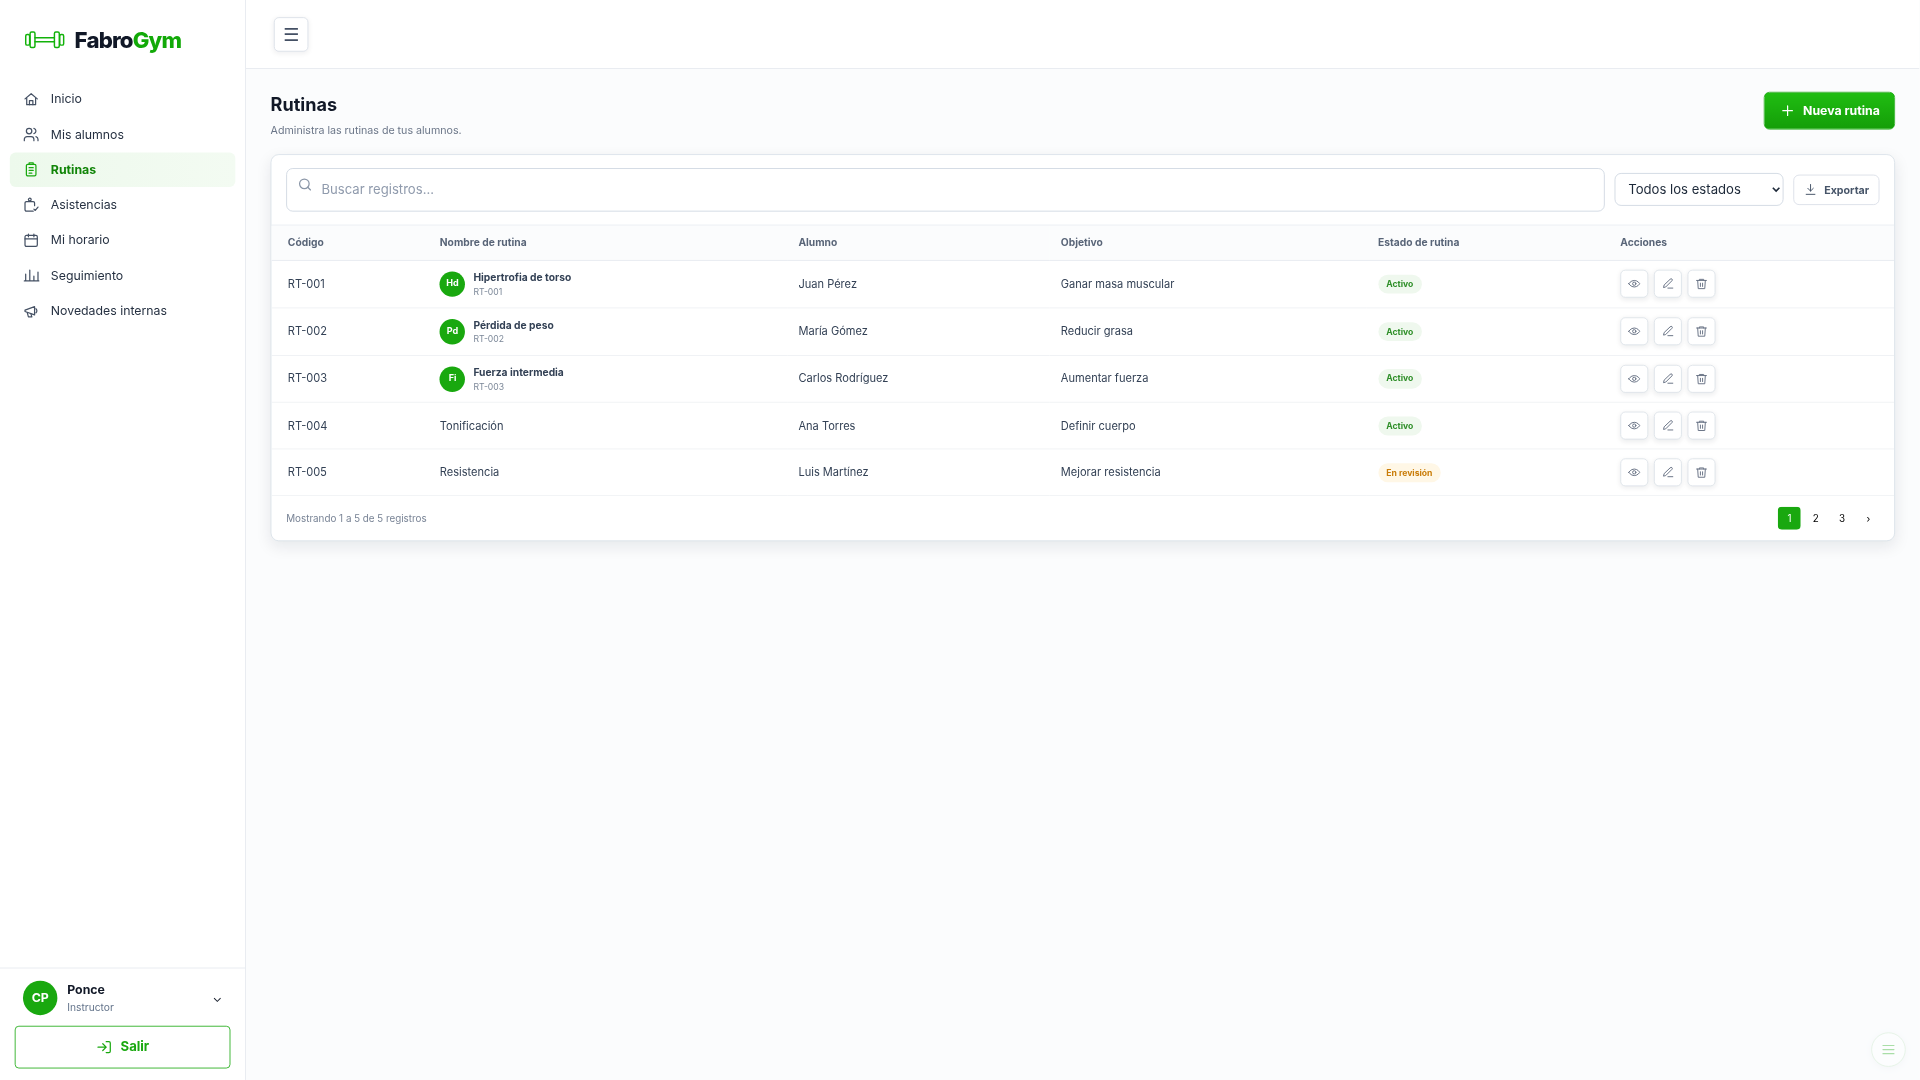
\includegraphics[width=.92\textwidth]{rutinas.png}\caption{Vista de gestión de rutinas del prototipo V7.}\end{figure}

\section{Validación}

\subsection{Diseño y corpus de validación}
Se analizaron tres sesiones técnicas independientes, identificadas públicamente como T01, T02 y T03. La matriz suministrada registra 39 fragmentos codificados, 18 hallazgos consolidados, 20 grupos de cambios revisados y ocho riesgos o discrepancias. Para M2 se verificó el cierre documental de las ocho discrepancias: ninguna permanece como contradicción entre requisitos de la línea base final. La validación se trató como walkthrough técnico apoyado en el prototipo V7 y se mantuvo la separación entre hallazgo, decisión y corrección recomendada \cite{sem11}.

\begin{alertbox}
La evidencia disponible no permite afirmar que la validación integral esté cerrada: no se aportaron tres walkthroughs no técnicos ni member checking. Asimismo, V7 es un prototipo HTML/JavaScript sin backend; respaldo, restauración e IA no se contabilizan como funciones implementadas. Estas limitaciones permanecen explícitas para no transformar ausencia de evidencia en un resultado ficticio.
\end{alertbox}

\begin{longtable}{|p{1.3cm}|p{4.6cm}|p{2.1cm}|p{7cm}|}
\caption{Tratamiento de los 18 hallazgos técnicos.}\\\hline
\textbf{ID} & \textbf{Hallazgo} & \textbf{Prioridad} & \textbf{Tratamiento}\\\hline\endfirsthead
\hline\textbf{ID} & \textbf{Hallazgo} & \textbf{Prioridad} & \textbf{Tratamiento}\\\hline\endhead
H01 & Portal del cliente & Alta & Adoptado: RF-MEM-05, RF-PAG-03 y RF-RUT-04 \\ \hline
H02 & Rutina personalizada y control humano & Alta & Adoptado y trazado en RF-RUT-01/02/04 y RF-IA-RUT-03 \\ \hline
H03 & IA como recomendador asistivo & Alta & Especificado con control humano y explicación; implementación pendiente \\ \hline
H04 & Claridad semántica de estados & Alta & Corregido mediante etiquetas contextuales y BDD \\ \hline
H05 & Navegación y jerarquía visual & Media-Alta & Conservar patrones V7 y verificar en walkthrough \\ \hline
H06 & Asistencia QR con contingencia manual & Alta & RF-ASI-01 modificado \\ \hline
H07 & Jerarquía de roles & Alta & RF-AUT-02 modificado a cinco roles \\ \hline
H08 & Auditoría de operaciones & Alta & RF-AUT-03 ampliado \\ \hline
H09 & Categorías y proveedores & Media-Alta & RF-INV-04 y RF-INV-05 añadidos \\ \hline
H10 & IVA configurable & Alta & RF-CFG-01 y RNF-FLE-01 \\ \hline
H11 & Analítica administrativa & Media & RF-REP-01 limitado a análisis descriptivo \\ \hline
H12 & Respaldo y recuperación & Alta & RF-BCK-01/02 y RNF-FIA-02; backend pendiente \\ \hline
H13 & Contacto mínimo & Alta & Teléfono opcional por minimización; discrepancia documentada \\ \hline
H14 & Formularios y validación & Alta & Criterios BDD y consistencia de formularios \\ \hline
H15 & Seguridad y transparencia & Media-Alta & Conservar transparencia; recuperación definitiva pendiente \\ \hline
H16 & Escalabilidad y mantenibilidad & Media-Alta & RNF-MAN-02 y RNF-FLE-01 \\ \hline
H17 & Pruebas con usuarios no técnicos & Crítica & Tratado como limitación de validación: existe protocolo preparado, pero no se declara sesión ejecutada \\ \hline
H18 & Clientes no tradicionales y pago flexible & Media & Conservado como decisión pendiente de negocio \\ \hline
\end{longtable}

\subsection{Conflictos y decisiones}
\begin{longtable}{|p{1.3cm}|p{4.4cm}|p{2.8cm}|p{7.2cm}|}
\caption{Conflictos, riesgos y decisión documentada.}\\\hline
\textbf{ID} & \textbf{Conflicto} & \textbf{Estado} & \textbf{Resolución o limitación}\\\hline\endfirsthead
\hline\textbf{ID} & \textbf{Conflicto} & \textbf{Estado} & \textbf{Resolución o limitación}\\\hline\endhead
I-01 & MU-66 vs minimización de datos & Resuelto & Se excluyen peso, grasa y masa corporal reales; solo seguimiento operativo no sensible. \\ \hline
I-02 & Rol Cliente futuro vs V7 & Resuelto & Se incorpora Cliente con funciones de consulta delimitadas. \\ \hline
I-03 & Tres roles vs cinco roles & Resuelto & RF-AUT-02 y matriz usan cinco roles. \\ \hline
I-04 & Validación técnica vs validación completa & Resuelto documentalmente & Se separa el resultado técnico de la limitación no técnica; el protocolo no ejecutado no se presenta como evidencia. \\ \hline
I-05 & IA requerida vs no implementada & Resuelto documentalmente & La IA queda especificada y trazada como alcance futuro; el prototipo actual no se presenta como implementación del modelo. \\ \hline
I-06 & Teléfono obligatorio vs opcional & Resuelto & Se mantiene opcional por minimización y se registra la discrepancia. \\ \hline
I-07 & Prototipo V7 vs MVP terminal & Resuelto documentalmente & V7 se etiqueta como prototipo HTML/JS; API, persistencia, respaldo e IA se mantienen como arquitectura objetivo. \\ \hline
I-08 & Correlación vs análisis descriptivo & Resuelto & RF-REP-01 usa indicadores descriptivos reproducibles. \\ \hline
\end{longtable}


\subsection{Cierre de conflictos y limitaciones}
Al cierre de la línea base v2.0 no se mantienen conflictos de requisitos abiertos. Los elementos I-04, I-05 e I-07 se cerraron por delimitación documental: continúan existiendo actividades no ejecutadas o componentes no implementados, pero ya no generan instrucciones contradictorias dentro del ERS. Esta separación permite que M2 mida consistencia del documento y no madurez de implementación.



\subsection{Protocolo de walkthrough con perfiles no técnicos}
Para una validación posterior con usuarios del dominio se define un protocolo moderado centrado en tareas observables. El propósito es comprobar comprensión del lenguaje, navegación, mensajes y correspondencia entre las tareas del gimnasio y las funciones especificadas. Este instrumento no modifica los resultados de las tres validaciones técnicas ni se contabiliza como sesión ejecutada.

\begin{longtable}{|p{2.7cm}|p{5.2cm}|p{4.2cm}|p{3.2cm}|}
\caption{Protocolo preparado para walkthrough no técnico.}\\\hline
\textbf{Perfil objetivo} & \textbf{Tareas propuestas} & \textbf{Criterio observable} & \textbf{Registro previsto}\\\hline\endfirsthead
\hline\textbf{Perfil objetivo} & \textbf{Tareas propuestas} & \textbf{Criterio observable} & \textbf{Registro previsto}\\\hline\endhead
Responsable del gimnasio & Consultar panel, revisar membresías, inventario y reportes & Completa al menos 9 de 10 tareas críticas sin ayuda & Observaciones, tiempo, errores y comentario final\\\hline
Recepción & Registrar cliente, activar membresía, pago, asistencia y venta & Identifica estados y mensajes sin explicación técnica & Secuencia seguida, dudas y propuestas de vocabulario\\\hline
Instructor & Crear, asignar, ajustar y consultar una rutina & Distingue versión vigente, historial y seguimiento & Incidencias, expectativas y decisión sobre cada hallazgo\\\hline
\end{longtable}

Cada sesión deberá ejecutarse sobre la misma versión del prototipo, utilizar un guion estable y convertir cada observación en un hallazgo trazable. Una recomendación solo se incorporará si el equipo documenta requisito afectado, decisión, responsable y cambio aplicado; este control evita transformar opiniones aisladas en requisitos aprobados.

\section{Gestión y trazabilidad}
El paquete documental PE5 se identifica como v2.0.3; los requisitos conservan el estado de aprobación de la línea base funcional v2.0. Cada RF dispone de una historia sincronizada y cada historia apunta a un RF existente, por lo que la sincronización documental del backlog propuesto es $40/40=100\%$. Este resultado no afirma que existiera previamente un tablero histórico; el archivo se entrega como reconstrucción controlada desde la ERS. La cadena mínima se verificó de acuerdo con la guía PE5 y con los principios de trazabilidad de ISO/IEC/IEEE 29148 e ISO/IEC/IEEE 15288 \cite{iso29148,iso15288}.
\begin{landscape}
\scriptsize
\begin{longtable}{|p{1.8cm}|p{3.4cm}|p{2.0cm}|p{1.4cm}|p{5.0cm}|p{4.0cm}|p{3.2cm}|}
\caption{Trazabilidad final, parte A: origen y realización en modelos.}\\
\hline\textbf{ID} & \textbf{Fuente} & \textbf{Actor} & \textbf{CU} & \textbf{Clase UML} & \textbf{Proceso DFD} & \textbf{Estado/transición}\\\hline\endfirsthead
\hline\textbf{ID} & \textbf{Fuente} & \textbf{Actor} & \textbf{CU} & \textbf{Clase UML} & \textbf{Proceso DFD} & \textbf{Estado/transición}\\\hline\endhead
RF-AUT-01 & EV-ENTR02-07 & Personal autorizado & CU-01 & Usuario; Rol; Permiso; EventoAuditoria & P-01 Controlar acceso & Sesión/permiso \\ \hline
RF-AUT-02 & EV-ENTR02-07;EV-ENTR03-06;EV-ENTR08-04 & Administrador & CU-02 & Usuario; Rol; Permiso; EventoAuditoria & P-01 Controlar acceso & Sesión/permiso \\ \hline
RF-AUT-03 & EV-ENTR02-04;EV-ENTR02-07;EV-ENTR03-06 & Administrador & CU-20 & Usuario; Rol; Permiso; EventoAuditoria & P-01 Controlar acceso & Sesión/permiso \\ \hline
RF-CLI-01 & EV-ENTR01-02;EV-ENTR02-02;EV-ENTR03-02;EV-ENTR08-01 & Recepcionista & CU-03 & Cliente; Membresia; Pago; Asistencia & P-02 Gestionar clientes & Cliente \\ \hline
RF-CLI-02 & EV-ENTR02-03;EV-ENTR02-08;EV-ENTR08-05 & Recepcionista & CU-04 & Cliente; Membresia; Pago; Asistencia & P-02 Gestionar clientes & Cliente \\ \hline
RF-CLI-03 & EV-ENTR02-02;EV-ENTR03-02;EV-ENTR04-01;EV-ENTR05-02 & Recepcionista & CU-05 & Cliente; Membresia; Pago; Asistencia & P-02 Gestionar clientes & Cliente \\ \hline
RF-MEM-01 & EV-ENTR02-01;EV-ENTR04-01 & Administrador & CU-06 & Membresia; Plan; Promocion & P-03 Gestionar membresías & Membresía \\ \hline
RF-MEM-02 & EV-ENTR01-02;EV-ENTR02-04;EV-ENTR03-01;EV-ENTR04-03 & Recepcionista & CU-07 & Membresia; Plan; Promocion & P-03 Gestionar membresías & Membresía \\ \hline
RF-MEM-03 & EV-ENTR01-03;EV-ENTR02-03;EV-ENTR03-03;EV-ENTR08-02 & Personal autorizado & CU-08 & Membresia; Plan; Promocion & P-03 Gestionar membresías & Membresía \\ \hline
RF-MEM-04 & EV-ENTR01-03;EV-ENTR05-02;EV-ENTR07-02 & Recepcionista & CU-09 & Membresia; Plan; Promocion & P-03 Gestionar membresías & Membresía \\ \hline
RF-PAG-01 & EV-ENTR01-02;EV-ENTR02-04;EV-ENTR03-04;EV-ENTR07-02;EV-ENTR08-03 & Recepcionista & CU-10 & Pago; Comprobante; Cliente & P-04 Gestionar pagos & Pago \\ \hline
RF-PAG-02 & EV-ENTR02-04;EV-ENTR03-04;EV-ENTR07-07 & Administrador & CU-21 & Pago; Comprobante; Cliente & P-04 Gestionar pagos & Pago \\ \hline
RF-ASI-01 & EV-ENTR02-03;EV-ENTR03-03;EV-ENTR04-02;EV-ENTR07-07;EV-ENTR08-02 & Recepcionista & CU-11 & Asistencia; Cliente; Turno & P-05 Controlar asistencia & Asistencia \\ \hline
RF-ASI-02 & EV-ENTR03-01;EV-ENTR07-01;EV-ENTR08-05;EV-ENTR09-06 & Personal autorizado & CU-12 & Asistencia; Cliente; Turno & P-05 Controlar asistencia & Asistencia \\ \hline
RF-INV-01 & EV-ENTR01-01;EV-ENTR02-05 & Administrador & CU-13 & Producto; Categoria; Proveedor; MovimientoStock & P-06 Gestionar inventario & Producto/stock \\ \hline
RF-INV-02 & EV-ENTR01-04;EV-ENTR04-04;EV-ENTR07-03 & Personal autorizado & CU-14 & Producto; Categoria; Proveedor; MovimientoStock & P-06 Gestionar inventario & Producto/stock \\ \hline
RF-VEN-01 & EV-ENTR02-05;EV-ENTR03-01;EV-ENTR04-04;EV-ENTR07-03;EV-ENTR08-03 & Recepcionista & CU-15 & Venta; DetalleVenta; Producto; Pago & P-07 Registrar ventas & Venta \\ \hline
RF-INV-03 & EV-ENTR01-04;EV-ENTR02-05;EV-ENTR05-04;EV-ENTR06-04 & Administrador & CU-22 & Producto; Categoria; Proveedor; MovimientoStock & P-06 Gestionar inventario & Producto/stock \\ \hline
RF-CAJ-01 & EV-ENTR02-01;EV-ENTR02-06;EV-ENTR03-05;EV-ENTR04-05;EV-ENTR07-03;EV-ENTR08-04 & Recepcionista & CU-16 & Caja; Turno; Venta; Pago & P-08 Conciliar caja & Turno de caja \\ \hline
RF-NOV-01 & EV-ENTR02-01;EV-ENTR02-08;EV-ENTR03-07;EV-ENTR04-06;EV-ENTR05-01 & Personal autorizado & CU-17 & Novedad; Usuario & P-09 Gestionar novedades & Novedad \\ \hline
RF-INS-01 & EV-ENTR07-06;EV-ENTR09-03;EV-ENTR10-02 & Administrador & CU-23 & Instructor; Horario; Cliente & P-10 Gestionar instructores & Horario \\ \hline
RF-RUT-01 & EV-ENTR01-05;EV-ENTR05-04;EV-ENTR09-01;EV-ENTR09-02;EV-ENTR09-03 & Instructor & CU-18 & Rutina; VersionRutina; Ejercicio; Cliente; Instructor & P-11 Gestionar rutinas & Rutina \\ \hline
RF-RUT-02 & EV-ENTR01-05;EV-ENTR09-01;EV-ENTR09-04;EV-ENTR10-01;EV-ENTR10-03 & Instructor & CU-19 & Rutina; VersionRutina; Ejercicio; Cliente; Instructor & P-11 Gestionar rutinas & Rutina \\ \hline
RF-RUT-03 & EV-ENTR09-04;EV-ENTR09-05;EV-ENTR09-06;EV-ENTR10-03;EV-ENTR10-04 & Instructor & CU-24 & Rutina; VersionRutina; Ejercicio; Cliente; Instructor & P-11 Gestionar rutinas & Rutina \\ \hline
RF-REP-01 & EV-ENTR01-05;EV-ENTR05-05;EV-ENTR06-04;EV-ENTR07-04;EV-ENTR08-05;EV-ENTR09-05 & Administrador & CU-25 & Reporte; Indicador; Filtro & P-12 Generar reportes & N/A (consulta) \\ \hline
RF-MEM-05 & EV-VT-T02-12; MU-63 & Cliente & CU-26 & Membresia; Plan; Promocion & P-03 Gestionar membresías & Membresía \\ \hline
RF-PAG-03 & EV-VT-T02-12 & Cliente & CU-27 & Pago; Comprobante; Cliente & P-04 Gestionar pagos & Pago \\ \hline
RF-RUT-04 & EV-VT-T01-06; EV-VT-T01-08; EV-VT-T02-04 & Cliente & CU-28 & Rutina; VersionRutina; Ejercicio; Cliente; Instructor & P-11 Gestionar rutinas & Rutina \\ \hline
RF-INV-04 & EV-VT-T03-06 & Dueño & CU-29 & Producto; Categoria; Proveedor; MovimientoStock & P-06 Gestionar inventario & Producto/stock \\ \hline
RF-INV-05 & EV-VT-T03-06; EV-VT-T01-10 & Dueño & CU-30 & Producto; Categoria; Proveedor; MovimientoStock & P-06 Gestionar inventario & Producto/stock \\ \hline
RF-CFG-01 & EV-VT-T03-05 & Dueño & CU-31 & Configuracion; HorarioAtencion; Producto & P-13 Configurar operación & Configuración \\ \hline
RF-BCK-01 & EV-VT-T03-10 & Superadministrador & CU-32 & Respaldo; EventoAuditoria & P-14 Respaldar y recuperar & Respaldo \\ \hline
RF-BCK-02 & EV-VT-T03-10 & Superadministrador & CU-33 & Respaldo; EventoAuditoria & P-14 Respaldar y recuperar & Respaldo \\ \hline
RF-CFG-02 & IND-14; V7 & Dueño & CU-34 & Configuracion; HorarioAtencion; Producto & P-13 Configurar operación & Configuración \\ \hline
RF-IA-RUT-01 & EV-VT-T02-05; H03; PE5-OE3 & Cliente/Instructor & CU-35 & ModeloIA; Recomendacion; Alerta; Explicacion & P-15 Asistir decisiones & Salida IA \\ \hline
RF-IA-RUT-02 & Decisión del equipo; PE5-OE3 & Cliente & CU-36 & ModeloIA; Recomendacion; Alerta; Explicacion & P-15 Asistir decisiones & Salida IA \\ \hline
RF-IA-RUT-03 & EV-VT-T01-07; EV-VT-T01-08; H02 & Instructor & CU-37 & ModeloIA; Recomendacion; Alerta; Explicacion & P-15 Asistir decisiones & Salida IA \\ \hline
RF-IA-ABA-01 & PE5-OE3; decisión de diseño & Dueño & CU-38 & ModeloIA; Recomendacion; Alerta; Explicacion & P-15 Asistir decisiones & Salida IA \\ \hline
RF-IA-ABA-02 & PE5-OE3; decisión de diseño & Dueño/Recepcionista & CU-39 & ModeloIA; Recomendacion; Alerta; Explicacion & P-15 Asistir decisiones & Salida IA \\ \hline
RF-IA-ABA-03 & PE5-OE3; decisión de diseño & Recepcionista & CU-40 & ModeloIA; Recomendacion; Alerta; Explicacion & P-15 Asistir decisiones & Salida IA \\ \hline
RNF-AF-01 & ISO/IEC 25010:2023; PE5 & Equipo/usuarios & N/A (transversal) & Componentes afectados & Procesos afectados & N/A (atributo de calidad) \\ \hline
RNF-ED-01 & ISO/IEC 25010:2023 & Equipo/usuarios & N/A (transversal) & Componentes afectados & Procesos afectados & N/A (atributo de calidad) \\ \hline
RNF-ED-02 & EV-VT-T01-03; EV-VT-T02-06; EV-VT-T03-08 & Equipo/usuarios & N/A (transversal) & Componentes afectados & Procesos afectados & N/A (atributo de calidad) \\ \hline
RNF-COM-01 & ISO/IEC 25010:2023 & Equipo/usuarios & N/A (transversal) & Componentes afectados & Procesos afectados & N/A (atributo de calidad) \\ \hline
RNF-IU-01 & EV-VT-T01-11; EV-VT-T01-12; H04; H05 & Equipo/usuarios & N/A (transversal) & Componentes afectados & Procesos afectados & N/A (atributo de calidad) \\ \hline
RNF-IU-02 & WCAG 2.2 & Equipo/usuarios & N/A (transversal) & Componentes afectados & Procesos afectados & N/A (atributo de calidad) \\ \hline
RNF-FIA-01 & ISO/IEC 25010:2023 & Equipo/usuarios & N/A (transversal) & Componentes afectados & Procesos afectados & N/A (atributo de calidad) \\ \hline
RNF-FIA-02 & EV-VT-T03-10; H12 & Equipo/usuarios & N/A (transversal) & Componentes afectados & Procesos afectados & N/A (atributo de calidad) \\ \hline
RNF-SEG-01 & LOPDP; RF-AUT-02 & Equipo/usuarios & N/A (transversal) & Componentes afectados & Procesos afectados & N/A (atributo de calidad) \\ \hline
RNF-SEG-02 & LOPDP; I-01 & Equipo/usuarios & N/A (transversal) & Componentes afectados & Procesos afectados & N/A (atributo de calidad) \\ \hline
RNF-SEG-03 & LOPDP; OWASP & Equipo/usuarios & N/A (transversal) & Componentes afectados & Procesos afectados & N/A (atributo de calidad) \\ \hline
RNF-MAN-01 & ISO/IEC 25010:2023 & Equipo/usuarios & N/A (transversal) & Componentes afectados & Procesos afectados & N/A (atributo de calidad) \\ \hline
RNF-MAN-02 & ISO/IEC 25010:2023; H16 & Equipo/usuarios & N/A (transversal) & Componentes afectados & Procesos afectados & N/A (atributo de calidad) \\ \hline
RNF-POR-01 & ISO/IEC 25010:2023 & Equipo/usuarios & N/A (transversal) & Componentes afectados & Procesos afectados & N/A (atributo de calidad) \\ \hline
RNF-FLE-01 & EV-VT-T03-05; H10; H16 & Equipo/usuarios & N/A (transversal) & Componentes afectados & Procesos afectados & N/A (atributo de calidad) \\ \hline
RNF-IA-RUT-P01 & PE5-OE3; ISO/IEC 25010:2023 & Equipo/usuarios & N/A (transversal) & ModeloIA; RegistroMetrica & Procesos afectados & N/A (atributo de calidad) \\ \hline
RNF-IA-RUT-P02 & PE5-OE3 & Equipo/usuarios & N/A (transversal) & ModeloIA; RegistroMetrica & Procesos afectados & N/A (atributo de calidad) \\ \hline
RNF-IA-RUT-P03 & PE5-OE3 & Equipo/usuarios & N/A (transversal) & ModeloIA; RegistroMetrica & Procesos afectados & N/A (atributo de calidad) \\ \hline
RNF-IA-RUT-E01 & PE5-OE3; Reglamento (UE) 2024/1689 & Equipo/usuarios & N/A (transversal) & ModeloIA; RegistroMetrica & Procesos afectados & N/A (atributo de calidad) \\ \hline
RNF-IA-RUT-E02 & PE5-OE3; LOPDP & Equipo/usuarios & N/A (transversal) & ModeloIA; RegistroMetrica & Procesos afectados & N/A (atributo de calidad) \\ \hline
RNF-IA-RUT-X01 & EV-VT-T02-05; H03 & Equipo/usuarios & N/A (transversal) & ModeloIA; RegistroMetrica & Procesos afectados & N/A (atributo de calidad) \\ \hline
RNF-IA-ABA-P01 & PE5-OE3 & Equipo/usuarios & N/A (transversal) & ModeloIA; RegistroMetrica & Procesos afectados & N/A (atributo de calidad) \\ \hline
RNF-IA-ABA-P02 & PE5-OE3 & Equipo/usuarios & N/A (transversal) & ModeloIA; RegistroMetrica & Procesos afectados & N/A (atributo de calidad) \\ \hline
RNF-IA-ABA-P03 & PE5-OE3 & Equipo/usuarios & N/A (transversal) & ModeloIA; RegistroMetrica & Procesos afectados & N/A (atributo de calidad) \\ \hline
RNF-IA-ABA-E01 & PE5-OE3; Reglamento (UE) 2024/1689 & Equipo/usuarios & N/A (transversal) & ModeloIA; RegistroMetrica & Procesos afectados & N/A (atributo de calidad) \\ \hline
RNF-IA-ABA-E02 & PE5-OE3 & Equipo/usuarios & N/A (transversal) & ModeloIA; RegistroMetrica & Procesos afectados & N/A (atributo de calidad) \\ \hline
RNF-IA-ABA-X01 & PE5-OE3 & Equipo/usuarios & N/A (transversal) & ModeloIA; RegistroMetrica & Procesos afectados & N/A (atributo de calidad) \\ \hline
\end{longtable}
\newpage
\begin{longtable}{|p{1.8cm}|p{11.8cm}|p{2.0cm}|p{2.0cm}|p{2.7cm}|p{2.0cm}|}
\caption{Trazabilidad final, parte B: aceptación, prueba y sincronización.}\\
\hline\textbf{ID} & \textbf{Criterio BDD} & \textbf{CP} & \textbf{Historia} & \textbf{Estado requisito} & \textbf{Estado traza}\\\hline\endfirsthead
\hline\textbf{ID} & \textbf{Criterio BDD} & \textbf{CP} & \textbf{Historia} & \textbf{Estado requisito} & \textbf{Estado traza}\\\hline\endhead
RF-AUT-01 & Dado un usuario con credenciales válidas, cuando inicie sesión, entonces el sistema deberá autenticarlo y habilitar únicamente las opciones permitidas para su rol; cuando cierre sesión, deberá invalidar la sesión activa. & CP-01 & HU-01 & Aprobado en baseline v2.0 & Completa \\ \hline
RF-AUT-02 & Dado un usuario autenticado con un rol definido, cuando intente ejecutar una operación, entonces el sistema deberá permitirla solo si el permiso está asignado a ese rol y deberá denegarla en caso contrario. & CP-02 & HU-02 & Aprobado en baseline v2.0 & Completa \\ \hline
RF-AUT-03 & Dado un cambio crítico confirmado, cuando el sistema lo registre, entonces deberá conservar en auditoría el actor, fecha, acción, valor anterior y valor nuevo asociados al cambio. & CP-20 & HU-20 & Aprobado en baseline v2.0 & Completa \\ \hline
RF-CLI-01 & Dado un formulario con código interno, nombre de uso y al menos un medio de contacto válido, cuando Recepción confirme el registro, entonces el sistema deberá crear un único cliente y no deberá solicitar datos de salud, biometría, dirección domiciliaria ni imagen corporal. & CP-03 & HU-03 & Aprobado en baseline v2.0 & Completa \\ \hline
RF-CLI-02 & Dado un criterio de búsqueda válido, cuando Recepción consulte un cliente, entonces el sistema deberá devolver las coincidencias y mostrar únicamente membresía, último pago, asistencia y novedades autorizadas por el rol. & CP-04 & HU-04 & Aprobado en baseline v2.0 & Completa \\ \hline
RF-CLI-03 & Dado que existe un cliente coincidente por código o contacto, cuando Recepción intente registrar o reactivar el perfil, entonces el sistema deberá advertir la coincidencia y permitir actualizar o reactivar el registro existente sin crear un duplicado. & CP-05 & HU-05 & Aprobado en baseline v2.0 & Completa \\ \hline
RF-MEM-01 & Dado un usuario autorizado y los datos obligatorios de un plan o promoción, cuando guarde la configuración, entonces el sistema deberá conservar nombre, duración, precio, vigencia y estado y deberá mostrar el registro actualizado. & CP-06 & HU-06 & Aprobado en baseline v2.0 & Completa \\ \hline
RF-MEM-02 & Dado un plan vigente y un pago confirmado, cuando Recepción active o renueve la membresía, entonces el sistema deberá calcular y guardar las fechas de inicio y vencimiento según la duración del plan. & CP-07 & HU-07 & Aprobado en baseline v2.0 & Completa \\ \hline
RF-MEM-03 & Dado un cliente con membresía registrada, cuando un usuario autorizado consulte su vigencia, entonces el sistema deberá mostrar estado, plan, fecha de inicio y fecha de vencimiento de la membresía seleccionada. & CP-08 & HU-08 & Aprobado en baseline v2.0 & Completa \\ \hline
RF-MEM-04 & Dado que existen membresías próximas a vencer o vencidas, cuando se ejecute la consulta diaria, entonces el sistema deberá separar las que vencen dentro de tres días de las ya vencidas y no deberá enviar mensajes externos de forma automática. & CP-09 & HU-09 & Aprobado en baseline v2.0 & Completa \\ \hline
RF-PAG-01 & Dado un pago con monto, concepto, medio, referencia y fecha válidos, cuando Recepción confirme el registro, entonces el sistema deberá guardar el pago y generar un comprobante interno vinculado al cliente. & CP-10 & HU-10 & Aprobado en baseline v2.0 & Completa \\ \hline
RF-PAG-02 & Dado un pago con estado pendiente, cuando un Administrador lo confirme, rechace o corrija, entonces el sistema deberá actualizar el estado y conservar el motivo y la evidencia de auditoría de la decisión. & CP-21 & HU-21 & Aprobado en baseline v2.0 & Completa \\ \hline
RF-ASI-01 & Dado un cliente identificado, cuando Recepción registre la asistencia por QR, entonces el sistema deberá guardar fecha, hora y método QR; si se utiliza contingencia manual, deberá exigir responsable y motivo. & CP-11 & HU-11 & Aprobado en baseline v2.0 & Completa \\ \hline
RF-ASI-02 & Dado un filtro por cliente, fecha o turno, cuando un usuario autorizado consulte asistencias, entonces el sistema deberá mostrar únicamente los registros que cumplan el filtro y los conteos correspondientes. & CP-12 & HU-12 & Aprobado en baseline v2.0 & Completa \\ \hline
RF-INV-01 & Dado un producto con código, nombre, precio, unidad, stock mínimo y estado válidos, cuando el Administrador confirme el registro, entonces el sistema deberá guardar el producto y permitir su consulta posterior. & CP-13 & HU-13 & Aprobado en baseline v2.0 & Completa \\ \hline
RF-INV-02 & Dado un producto existente y un movimiento válido, cuando un usuario autorizado registre una entrada o ajuste, entonces el sistema deberá actualizar el saldo y conservar cantidad, motivo, responsable y saldo resultante. & CP-14 & HU-14 & Aprobado en baseline v2.0 & Completa \\ \hline
RF-VEN-01 & Dado que todos los ítems de una venta tienen stock suficiente, cuando Recepción confirme la venta, entonces el sistema deberá registrar la venta y descontar las existencias en una única transacción; si falla una operación, no deberá aplicar cambios parciales. & CP-15 & HU-15 & Aprobado en baseline v2.0 & Completa \\ \hline
RF-INV-03 & Dado un período de consulta, cuando el Administrador solicite el control de stock, entonces el sistema deberá listar los productos con stock igual o inferior al mínimo y resumir entradas, salidas y ventas del período. & CP-22 & HU-22 & Aprobado en baseline v2.0 & Completa \\ \hline
RF-CAJ-01 & Dado un turno con pagos y ventas registrados, cuando Recepción ejecute el cierre, entonces el sistema deberá totalizar por medio de pago, comparar contra los valores declarados y registrar cualquier diferencia junto con la entrega del turno. & CP-16 & HU-16 & Aprobado en baseline v2.0 & Completa \\ \hline
RF-NOV-01 & Dado un usuario autorizado y una novedad con categoría, detalle, responsable y vencimiento, cuando la registre, entonces el sistema deberá crearla con un estado válido y conservar los cambios posteriores de estado. & CP-17 & HU-17 & Aprobado en baseline v2.0 & Completa \\ \hline
RF-INS-01 & Dado un instructor registrado, cuando el Administrador actualice su operación, entonces el sistema deberá guardar turnos, capacidad, disponibilidad y novedades operativas sin solicitar datos de salud. & CP-23 & HU-23 & Aprobado en baseline v2.0 & Completa \\ \hline
RF-RUT-01 & Dado un cliente autorizado y un catálogo de ejercicios disponible, cuando el Instructor cree una rutina, entonces el sistema deberá guardar objetivo operativo, ejercicios, series, repeticiones, descanso y días, y deberá asignarla al cliente seleccionado. & CP-18 & HU-18 & Aprobado en baseline v2.0 & Completa \\ \hline
RF-RUT-02 & Dado una rutina existente, cuando el Instructor modifique ejercicios o parámetros y confirme el cambio, entonces el sistema deberá crear una nueva versión y mantener las versiones anteriores en solo lectura. & CP-19 & HU-19 & Aprobado en baseline v2.0 & Completa \\ \hline
RF-RUT-03 & Dado una rutina activa, cuando el Instructor registre seguimiento, entonces el sistema deberá guardar fecha, cumplimiento, repeticiones y observación operativa y deberá rechazar campos destinados a diagnósticos, lesiones, peso o medidas corporales reales. & CP-24 & HU-24 & Aprobado en baseline v2.0 & Completa \\ \hline
RF-REP-01 & Dado un período y filtros válidos, cuando el Administrador consulte el panel o reporte, entonces el sistema deberá calcular los indicadores con datos almacenados, mostrar los resultados filtrados y permitir exportarlos a CSV. & CP-25 & HU-25 & Aprobado en baseline v2.0 & Completa \\ \hline
RF-MEM-05 & Dado un Cliente autenticado, cuando consulte su membresía, entonces el sistema deberá mostrar únicamente el estado, plan y vigencia de su propia membresía y no deberá habilitar edición. & CP-26 & HU-26 & Aprobado en baseline v2.0 & Completa \\ \hline
RF-PAG-03 & Dado un Cliente autenticado, cuando consulte sus pagos, entonces el sistema deberá mostrar únicamente sus registros de pago y el estado de cada uno en modo de solo lectura. & CP-27 & HU-27 & Aprobado en baseline v2.0 & Completa \\ \hline
RF-RUT-04 & Dado un Cliente autenticado con una rutina asignada, cuando consulte su rutina, entonces el sistema deberá mostrar la versión activa, las versiones históricas y el seguimiento autorizado sin permitir modificar la rutina vigente. & CP-28 & HU-28 & Aprobado en baseline v2.0 & Completa \\ \hline
RF-INV-04 & Dado un usuario autorizado, cuando registre, edite o desactive una categoría, entonces el sistema deberá guardar el cambio y reflejar el estado actualizado en las consultas de categorías. & CP-29 & HU-29 & Aprobado en baseline v2.0 & Completa \\ \hline
RF-INV-05 & Dado un usuario autorizado, cuando registre, edite o desactive un proveedor, entonces el sistema deberá guardar el cambio y reflejar el estado actualizado en las consultas de proveedores. & CP-30 & HU-30 & Aprobado en baseline v2.0 & Completa \\ \hline
RF-CFG-01 & Dado un porcentaje de IVA válido y la configuración tributaria de un producto, cuando el Dueño confirme el cambio, entonces el sistema deberá aplicar la nueva configuración a operaciones posteriores y conservar el valor anterior, el nuevo valor, el actor y la fecha. & CP-31 & HU-31 & Aprobado en baseline v2.0 & Completa \\ \hline
RF-BCK-01 & Dado un Superadministrador autenticado, cuando solicite un respaldo, entonces el sistema deberá iniciar el proceso cifrado, asignar un identificador y mostrar el estado y la fecha de finalización cuando concluya. & CP-32 & HU-32 & Aprobado en baseline v2.0 & Completa \\ \hline
RF-BCK-02 & Dado un respaldo íntegro seleccionado, cuando el Superadministrador confirme explícitamente la restauración, entonces el sistema deberá verificar su integridad, ejecutar la restauración y registrar la operación en auditoría; si la verificación falla, no deberá restaurar. & CP-33 & HU-33 & Aprobado en baseline v2.0 & Completa \\ \hline
RF-CFG-02 & Dado un Dueño autenticado y una configuración válida de días y horas, cuando guarde el horario, entonces el sistema deberá actualizarlo y mostrar al Cliente únicamente el horario vigente. & CP-34 & HU-34 & Aprobado en baseline v2.0 & Completa \\ \hline
RF-IA-RUT-01 & Dado un objetivo operativo, disponibilidad semanal, historial no sensible y catálogo autorizado, cuando se solicite una recomendación, entonces el componente deberá devolver como máximo tres alternativas ordenadas de rutina y una explicación de los factores utilizados. & CP-35 & HU-35 & Aprobado como requisito PE5; implementación pendiente & Completa \\ \hline
RF-IA-RUT-02 & Dado que el Cliente visualiza una recomendación de rutina, cuando seleccione aceptar, rechazar o solicitar alternativa, entonces el sistema deberá registrar la decisión y no deberá activar automáticamente la recomendación. & CP-36 & HU-36 & Aprobado como requisito PE5; implementación pendiente & Completa \\ \hline
RF-IA-RUT-03 & Dado una recomendación aceptada por el Cliente, cuando el Instructor la revise, entonces el sistema deberá permitir aprobarla o rechazarla con motivo; únicamente una aprobación explícita podrá habilitar su activación. & CP-37 & HU-37 & Aprobado como requisito PE5; implementación pendiente & Completa \\ \hline
RF-IA-ABA-01 & Dado el historial de asistencia, vigencia de membresía y frecuencia histórica de un cliente, cuando se ejecute el cálculo semanal, entonces el componente deberá asignar un nivel bajo, medio o alto y registrar la fecha del cálculo. & CP-38 & HU-38 & Aprobado como requisito PE5; implementación pendiente & Completa \\ \hline
RF-IA-ABA-02 & Dado que existen clientes clasificados con riesgo medio o alto, cuando Dueño o Recepcionista consulte las alertas, entonces el sistema deberá mostrar el nivel, la fecha y los principales factores de cada alerta sin ejecutar acciones automáticas. & CP-39 & HU-39 & Aprobado como requisito PE5; implementación pendiente & Completa \\ \hline
RF-IA-ABA-03 & Dado una alerta de riesgo visible, cuando Recepción registre contacto, aplazamiento o descarte, entonces el sistema deberá guardar la acción, responsable, fecha y observación para auditoría. & CP-40 & HU-40 & Aprobado como requisito PE5; implementación pendiente & Completa \\ \hline
RNF-AF-01 & Dado un entorno de prueba reproducible, cuando se ejecute el método de comprobación definido para RNF-AF-01, entonces se deberá alcanzar el umbral expresado en el requisito y conservar la evidencia. & CP-RNF-AF-01 & HUQ-RNF-AF-01 & Especificado; verificación pendiente & Completa \\ \hline
RNF-ED-01 & Dado un entorno de prueba reproducible, cuando se ejecute el método de comprobación definido para RNF-ED-01, entonces se deberá alcanzar el umbral expresado en el requisito y conservar la evidencia. & CP-RNF-ED-01 & HUQ-RNF-ED-01 & Especificado; verificación pendiente & Completa \\ \hline
RNF-ED-02 & Dado un entorno de prueba reproducible, cuando se ejecute el método de comprobación definido para RNF-ED-02, entonces se deberá alcanzar el umbral expresado en el requisito y conservar la evidencia. & CP-RNF-ED-02 & HUQ-RNF-ED-02 & Especificado; verificación pendiente & Completa \\ \hline
RNF-COM-01 & Dado un entorno de prueba reproducible, cuando se ejecute el método de comprobación definido para RNF-COM-01, entonces se deberá alcanzar el umbral expresado en el requisito y conservar la evidencia. & CP-RNF-COM-01 & HUQ-RNF-COM-01 & Especificado; verificación pendiente & Completa \\ \hline
RNF-IU-01 & Dado un entorno de prueba reproducible, cuando se ejecute el método de comprobación definido para RNF-IU-01, entonces se deberá alcanzar el umbral expresado en el requisito y conservar la evidencia. & CP-RNF-IU-01 & HUQ-RNF-IU-01 & Especificado; verificación pendiente & Completa \\ \hline
RNF-IU-02 & Dado un entorno de prueba reproducible, cuando se ejecute el método de comprobación definido para RNF-IU-02, entonces se deberá alcanzar el umbral expresado en el requisito y conservar la evidencia. & CP-RNF-IU-02 & HUQ-RNF-IU-02 & Especificado; verificación pendiente & Completa \\ \hline
RNF-FIA-01 & Dado un entorno de prueba reproducible, cuando se ejecute el método de comprobación definido para RNF-FIA-01, entonces se deberá alcanzar el umbral expresado en el requisito y conservar la evidencia. & CP-RNF-FIA-01 & HUQ-RNF-FIA-01 & Especificado; verificación pendiente & Completa \\ \hline
RNF-FIA-02 & Dado un entorno de prueba reproducible, cuando se ejecute el método de comprobación definido para RNF-FIA-02, entonces se deberá alcanzar el umbral expresado en el requisito y conservar la evidencia. & CP-RNF-FIA-02 & HUQ-RNF-FIA-02 & Especificado; verificación pendiente & Completa \\ \hline
RNF-SEG-01 & Dado un entorno de prueba reproducible, cuando se ejecute el método de comprobación definido para RNF-SEG-01, entonces se deberá alcanzar el umbral expresado en el requisito y conservar la evidencia. & CP-RNF-SEG-01 & HUQ-RNF-SEG-01 & Especificado; verificación pendiente & Completa \\ \hline
RNF-SEG-02 & Dado un entorno de prueba reproducible, cuando se ejecute el método de comprobación definido para RNF-SEG-02, entonces se deberá alcanzar el umbral expresado en el requisito y conservar la evidencia. & CP-RNF-SEG-02 & HUQ-RNF-SEG-02 & Especificado; verificación pendiente & Completa \\ \hline
RNF-SEG-03 & Dado un entorno de prueba reproducible, cuando se ejecute el método de comprobación definido para RNF-SEG-03, entonces se deberá alcanzar el umbral expresado en el requisito y conservar la evidencia. & CP-RNF-SEG-03 & HUQ-RNF-SEG-03 & Especificado; verificación pendiente & Completa \\ \hline
RNF-MAN-01 & Dado un entorno de prueba reproducible, cuando se ejecute el método de comprobación definido para RNF-MAN-01, entonces se deberá alcanzar el umbral expresado en el requisito y conservar la evidencia. & CP-RNF-MAN-01 & HUQ-RNF-MAN-01 & Especificado; verificación pendiente & Completa \\ \hline
RNF-MAN-02 & Dado un entorno de prueba reproducible, cuando se ejecute el método de comprobación definido para RNF-MAN-02, entonces se deberá alcanzar el umbral expresado en el requisito y conservar la evidencia. & CP-RNF-MAN-02 & HUQ-RNF-MAN-02 & Especificado; verificación pendiente & Completa \\ \hline
RNF-POR-01 & Dado un entorno de prueba reproducible, cuando se ejecute el método de comprobación definido para RNF-POR-01, entonces se deberá alcanzar el umbral expresado en el requisito y conservar la evidencia. & CP-RNF-POR-01 & HUQ-RNF-POR-01 & Especificado; verificación pendiente & Completa \\ \hline
RNF-FLE-01 & Dado un entorno de prueba reproducible, cuando se ejecute el método de comprobación definido para RNF-FLE-01, entonces se deberá alcanzar el umbral expresado en el requisito y conservar la evidencia. & CP-RNF-FLE-01 & HUQ-RNF-FLE-01 & Especificado; verificación pendiente & Completa \\ \hline
RNF-IA-RUT-P01 & Dado un entorno de prueba reproducible, cuando se ejecute el método de comprobación definido para RNF-IA-RUT-P01, entonces se deberá alcanzar el umbral expresado en el requisito y conservar la evidencia. & CP-RNF-IA-RUT-P01 & HUQ-RNF-IA-RUT-P01 & Aprobado como requisito PE5; evaluación pendiente & Completa \\ \hline
RNF-IA-RUT-P02 & Dado un entorno de prueba reproducible, cuando se ejecute el método de comprobación definido para RNF-IA-RUT-P02, entonces se deberá alcanzar el umbral expresado en el requisito y conservar la evidencia. & CP-RNF-IA-RUT-P02 & HUQ-RNF-IA-RUT-P02 & Aprobado como requisito PE5; evaluación pendiente & Completa \\ \hline
RNF-IA-RUT-P03 & Dado un entorno de prueba reproducible, cuando se ejecute el método de comprobación definido para RNF-IA-RUT-P03, entonces se deberá alcanzar el umbral expresado en el requisito y conservar la evidencia. & CP-RNF-IA-RUT-P03 & HUQ-RNF-IA-RUT-P03 & Aprobado como requisito PE5; evaluación pendiente & Completa \\ \hline
RNF-IA-RUT-E01 & Dado un entorno de prueba reproducible, cuando se ejecute el método de comprobación definido para RNF-IA-RUT-E01, entonces se deberá alcanzar el umbral expresado en el requisito y conservar la evidencia. & CP-RNF-IA-RUT-E01 & HUQ-RNF-IA-RUT-E01 & Aprobado como requisito PE5; evaluación pendiente & Completa \\ \hline
RNF-IA-RUT-E02 & Dado un entorno de prueba reproducible, cuando se ejecute el método de comprobación definido para RNF-IA-RUT-E02, entonces se deberá alcanzar el umbral expresado en el requisito y conservar la evidencia. & CP-RNF-IA-RUT-E02 & HUQ-RNF-IA-RUT-E02 & Aprobado como requisito PE5; evaluación pendiente & Completa \\ \hline
RNF-IA-RUT-X01 & Dado un entorno de prueba reproducible, cuando se ejecute el método de comprobación definido para RNF-IA-RUT-X01, entonces se deberá alcanzar el umbral expresado en el requisito y conservar la evidencia. & CP-RNF-IA-RUT-X01 & HUQ-RNF-IA-RUT-X01 & Aprobado como requisito PE5; evaluación pendiente & Completa \\ \hline
RNF-IA-ABA-P01 & Dado un entorno de prueba reproducible, cuando se ejecute el método de comprobación definido para RNF-IA-ABA-P01, entonces se deberá alcanzar el umbral expresado en el requisito y conservar la evidencia. & CP-RNF-IA-ABA-P01 & HUQ-RNF-IA-ABA-P01 & Aprobado como requisito PE5; evaluación pendiente & Completa \\ \hline
RNF-IA-ABA-P02 & Dado un entorno de prueba reproducible, cuando se ejecute el método de comprobación definido para RNF-IA-ABA-P02, entonces se deberá alcanzar el umbral expresado en el requisito y conservar la evidencia. & CP-RNF-IA-ABA-P02 & HUQ-RNF-IA-ABA-P02 & Aprobado como requisito PE5; evaluación pendiente & Completa \\ \hline
RNF-IA-ABA-P03 & Dado un entorno de prueba reproducible, cuando se ejecute el método de comprobación definido para RNF-IA-ABA-P03, entonces se deberá alcanzar el umbral expresado en el requisito y conservar la evidencia. & CP-RNF-IA-ABA-P03 & HUQ-RNF-IA-ABA-P03 & Aprobado como requisito PE5; evaluación pendiente & Completa \\ \hline
RNF-IA-ABA-E01 & Dado un entorno de prueba reproducible, cuando se ejecute el método de comprobación definido para RNF-IA-ABA-E01, entonces se deberá alcanzar el umbral expresado en el requisito y conservar la evidencia. & CP-RNF-IA-ABA-E01 & HUQ-RNF-IA-ABA-E01 & Aprobado como requisito PE5; evaluación pendiente & Completa \\ \hline
RNF-IA-ABA-E02 & Dado un entorno de prueba reproducible, cuando se ejecute el método de comprobación definido para RNF-IA-ABA-E02, entonces se deberá alcanzar el umbral expresado en el requisito y conservar la evidencia. & CP-RNF-IA-ABA-E02 & HUQ-RNF-IA-ABA-E02 & Aprobado como requisito PE5; evaluación pendiente & Completa \\ \hline
RNF-IA-ABA-X01 & Dado un entorno de prueba reproducible, cuando se ejecute el método de comprobación definido para RNF-IA-ABA-X01, entonces se deberá alcanzar el umbral expresado en el requisito y conservar la evidencia. & CP-RNF-IA-ABA-X01 & HUQ-RNF-IA-ABA-X01 & Aprobado como requisito PE5; evaluación pendiente & Completa \\ \hline
\end{longtable}
\normalsize
\end{landscape}

\subsection{Control explícito de huérfanos y cadenas rotas}
\begin{longtable}{|p{4.1cm}|p{2.1cm}|p{5.1cm}|p{4.2cm}|}\hline
\textbf{Patología} & \textbf{Cantidad final} & \textbf{Criterio de revisión} & \textbf{Acción al cierre}\\\hline
Requisitos sin fuente & 0 & Toda fila RF conserva evidencia, norma o decisión de diseño en la columna Fuente. & No aplica; cobertura $40/40$.\\\hline
RF sin realización posterior & 0 & Todo RF enlaza CU, clase, proceso/estado, BDD y CP. & No aplica; M4 adelante $40/40$.\\\hline
Artefactos huérfanos de CU & 0 & CU-01 a CU-40 están vinculados uno a uno con RF del catálogo. & No aplica; catálogo sincronizado.\\\hline
Cadenas rotas & 0 & La columna Estado de traza no contiene estados ``rota'' ni ``huérfana''. & Cadenas incompletas de la línea base anterior fueron enlazadas o delimitadas.\\\hline
\end{longtable}


\begin{landscape}
\begin{figure}[H]\centering
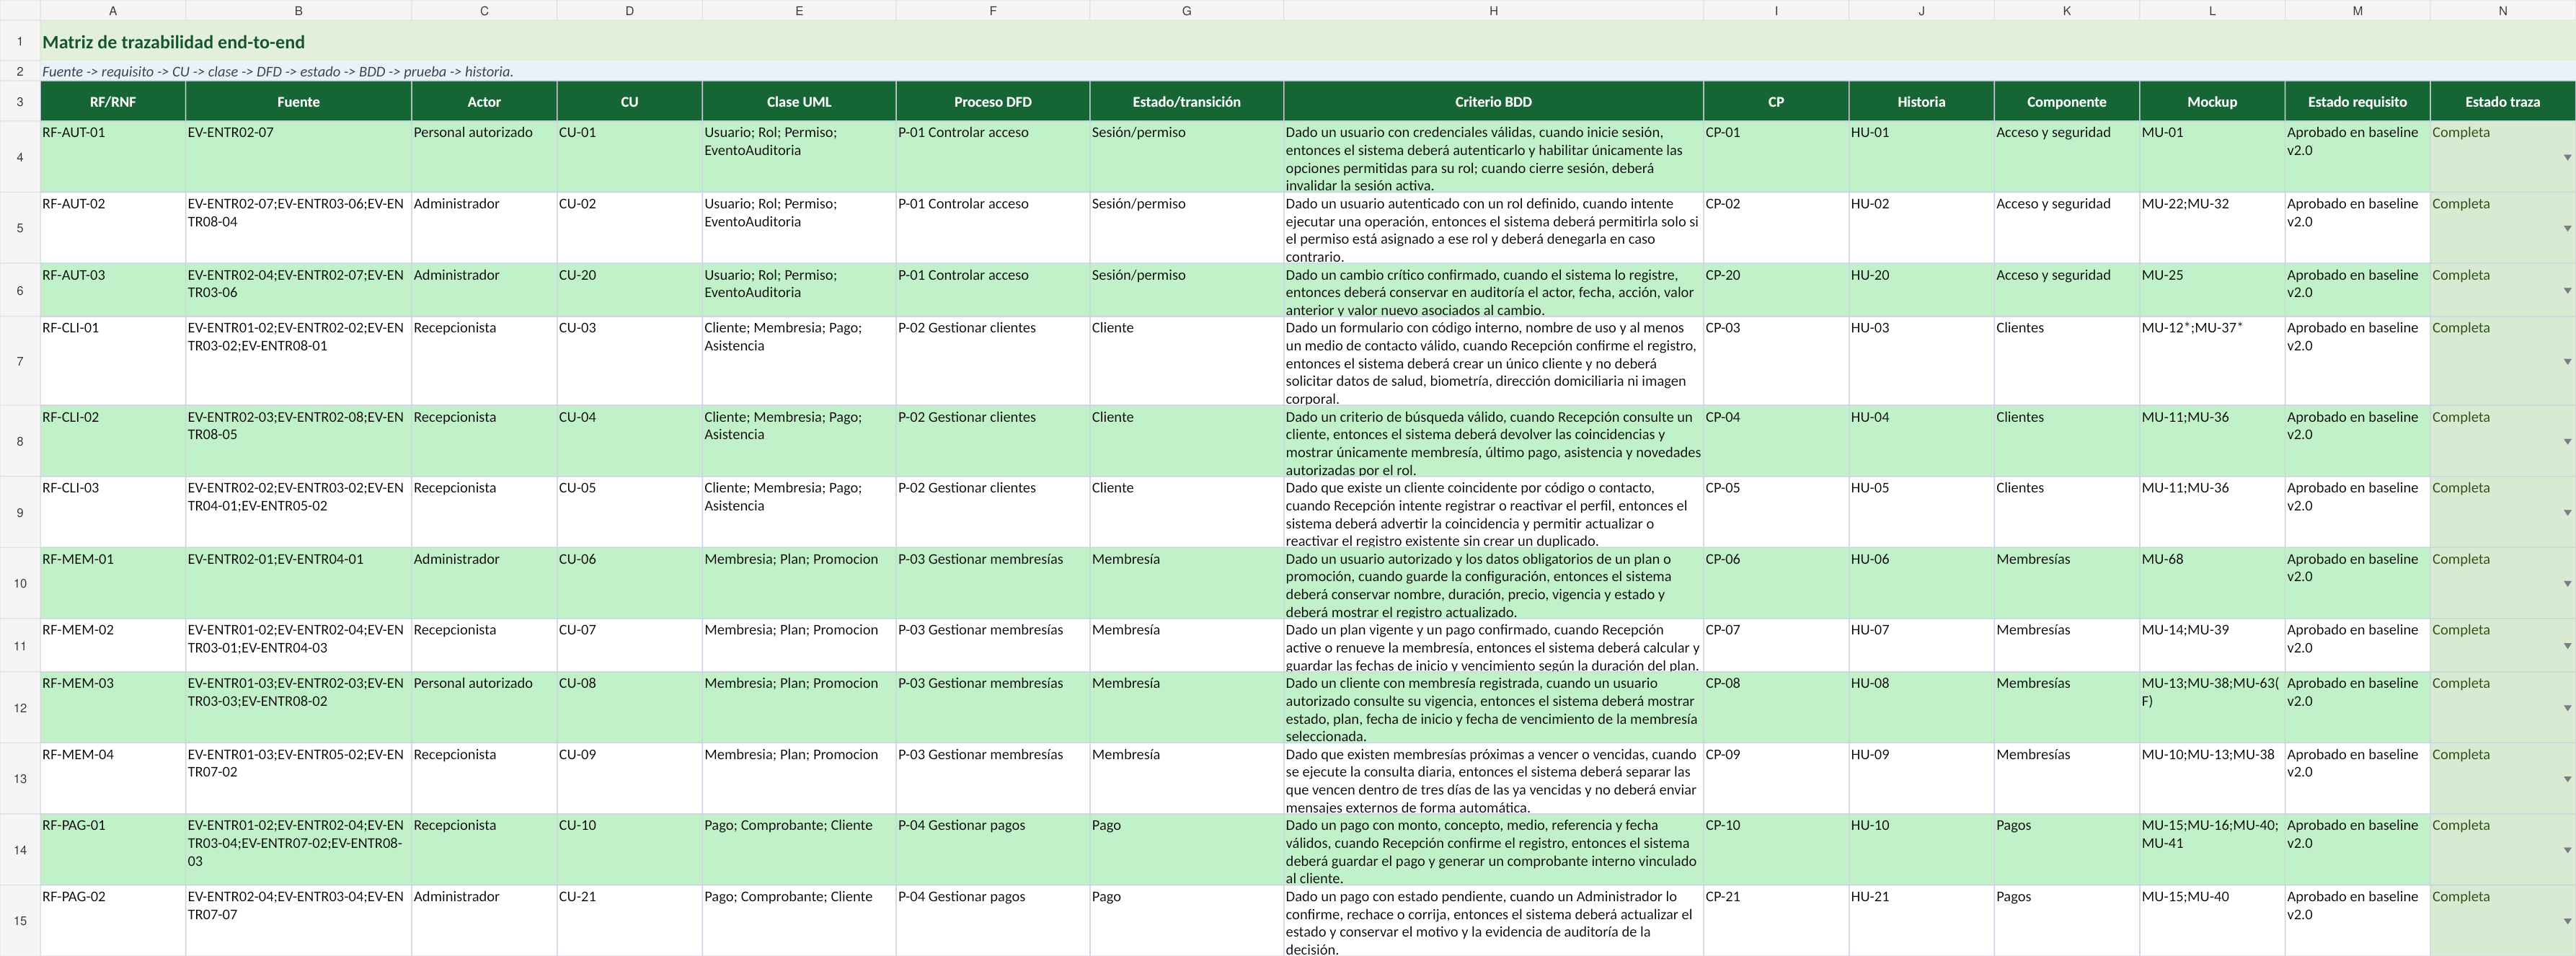
\includegraphics[width=.98\linewidth]{matriz_trazabilidad_vista.png}
\caption{Vista numerada de la matriz de trazabilidad final. La versión completa de 67 filas permanece en el archivo Excel y en el anexo paginado.}
\end{figure}
\end{landscape}

La figura permite reconocer la estructura Fuente $\rightarrow$ RF $\rightarrow$ actor $\rightarrow$ CU $\rightarrow$ clase $\rightarrow$ proceso $\rightarrow$ estado $\rightarrow$ BDD $\rightarrow$ CP $\rightarrow$ historia. Para verificar valores concretos debe utilizarse la matriz editable, porque una captura panorámica no reemplaza las celdas auditables ni sus fórmulas.

\section{Requisitos de inteligencia artificial}

\subsection{Principios comunes y base de legitimación}
Los componentes de IA se especifican como apoyo a decisiones y no como autoridad autónoma. La LOPDP exige que cada finalidad de tratamiento se sustente en una base de legitimación aplicable \cite{lopdp,spdp}. Para FabroGym se adopta, como diseño jurídico preliminar sujeto a validación por el responsable real del tratamiento, la siguiente separación: (i) los datos estrictamente necesarios para gestionar membresías, pagos, asistencia y prestación del servicio se vinculan a medidas precontractuales o al cumplimiento de la relación contractual; (ii) la personalización opcional mediante IA-01 y cualquier uso secundario no necesario para prestar el servicio requerirá consentimiento específico, informado y revocable; y (iii) no se presumirá interés legítimo para analítica o seguimiento sin una evaluación previa de ponderación y documentación de la finalidad.

El Reglamento (UE) 2024/1689 se emplea únicamente como referente comparado de gestión de riesgos, transparencia y supervisión humana \cite{aiact}; no se presenta como norma ecuatoriana aplicable. Ningún componente utiliza salud, diagnósticos, biometría, peso, grasa, masa muscular ni imagen corporal real. Durante desarrollo se emplearán datos sintéticos o datos operativos cuya base de legitimación, finalidad y período de conservación estén documentados antes del tratamiento.

\begin{table}[H]
\centering
\caption{Controles de privacidad y derechos aplicables a los componentes de IA.}
\small
\begin{tabularx}{\textwidth}{|p{3.2cm}|Y|Y|}
\hline
\textbf{Control} & \textbf{Requisito de diseño} & \textbf{Evidencia prevista}\\\hline
Finalidad & Separar gestión contractual, personalización opcional y seguimiento administrativo; prohibir reutilización para finalidades incompatibles. & Inventario de tratamientos y aviso de privacidad versionado.\\\hline
Minimización & Usar únicamente variables operativas necesarias y excluir datos sensibles de salud o biometría. & Diccionario de datos y revisión de campos por componente.\\\hline
Conservación & Definir un plazo por finalidad antes de producción; al vencimiento, eliminar o anonimizar de forma verificable. & Política de conservación aprobada y registro de eliminación.\\\hline
Derechos del titular & Habilitar canales para información, acceso, rectificación, actualización, eliminación y oposición cuando correspondan. & Registro de solicitudes y respuesta del responsable.\\\hline
Supervisión humana & Ninguna recomendación o alerta producirá activación, restricción del servicio o efecto automático irreversible. & Log de decisión humana y motivo.\\\hline
\end{tabularx}
\end{table}

Los requisitos de datos, métricas, monitoreo y explicación se documentan como parte del comportamiento esperado del sistema con IA, en línea con la literatura de Ingeniería de Requisitos para aprendizaje automático \cite{vogelsang}.

\subsection{IA-01: recomendador asistivo de rutinas}
\begin{tabularx}{\textwidth}{>{\bfseries}p{3.8cm}Y}
Tarea & Ordenar hasta tres alternativas de rutina; la activación exige decisión del cliente y revisión del instructor.\\
Entradas & Objetivo operativo declarado, disponibilidad semanal, historial de cumplimiento no sensible y catálogo autorizado.\\
Salida & Alternativas ordenadas con ejercicios, frecuencia y explicación; nunca prescripción médica.\\
Datos & Al menos 300 casos sintéticos revisados por instructores, versionados y separados en entrenamiento, validación y prueba.\\
Métrica principal & Precisión top-3 mayor o igual a 0,80; latencia p95 menor o igual a 800 ms.\\
Equidad & Brecha máxima de 5 puntos porcentuales entre rangos etarios y, cuando exista muestra suficiente, por género declarado.\\
Explicabilidad & Tres factores determinantes y restricciones aplicadas antes de aceptar.\\
Fallback & Creación manual por instructor; ninguna recomendación se activa automáticamente.\\
Monitoreo & Medición mensual; alerta si la precisión cae más de 5 puntos o una brecha supera 5 puntos; revisión antes de reentrenar.\\
Riesgo & No se clasifica como alto riesgo según el uso previsto; se mantiene supervisión humana y transparencia.\\
\end{tabularx}

\subsection{IA-02: detector de riesgo de inactividad}
\begin{tabularx}{\textwidth}{>{\bfseries}p{3.8cm}Y}
Tarea & Clasificar semanalmente riesgo bajo, medio o alto para priorizar seguimiento administrativo.\\
Entradas & Asistencia, vigencia de membresía y frecuencia histórica; se excluyen datos sensibles.\\
Salida & Nivel de riesgo, fecha y dos factores operativos principales.\\
Datos & Al menos 500 casos sintéticos con separación temporal para evaluación.\\
Métrica principal & F1 mayor o igual a 0,80 para riesgo alto; lote de 10 000 clientes en 10 minutos o menos.\\
Equidad & Brecha de falsos positivos menor o igual a 5 puntos porcentuales por edad y tipo de membresía.\\
Explicabilidad & Dos factores, ventana temporal y advertencia de que la alerta no es decisión definitiva.\\
Fallback & Mantener último cálculo con fecha visible; la decisión de contacto corresponde al personal.\\
Monitoreo & Medición mensual de F1, falsos positivos y deriva; revisión si F1 cae bajo 0,80.\\
Riesgo & Uso administrativo de apoyo, sin negar servicios ni producir efectos jurídicos automáticos.\\
\end{tabularx}

\begin{alertbox}
Los componentes IA-01 e IA-02 están especificados y trazados para PE5, pero no están implementados en V7. Antes de producción requieren prototipo, validación con clientes e instructores, evaluación del conjunto de datos, análisis de impacto de privacidad y pruebas de seguridad.
\end{alertbox}

\begin{figure}[H]\centering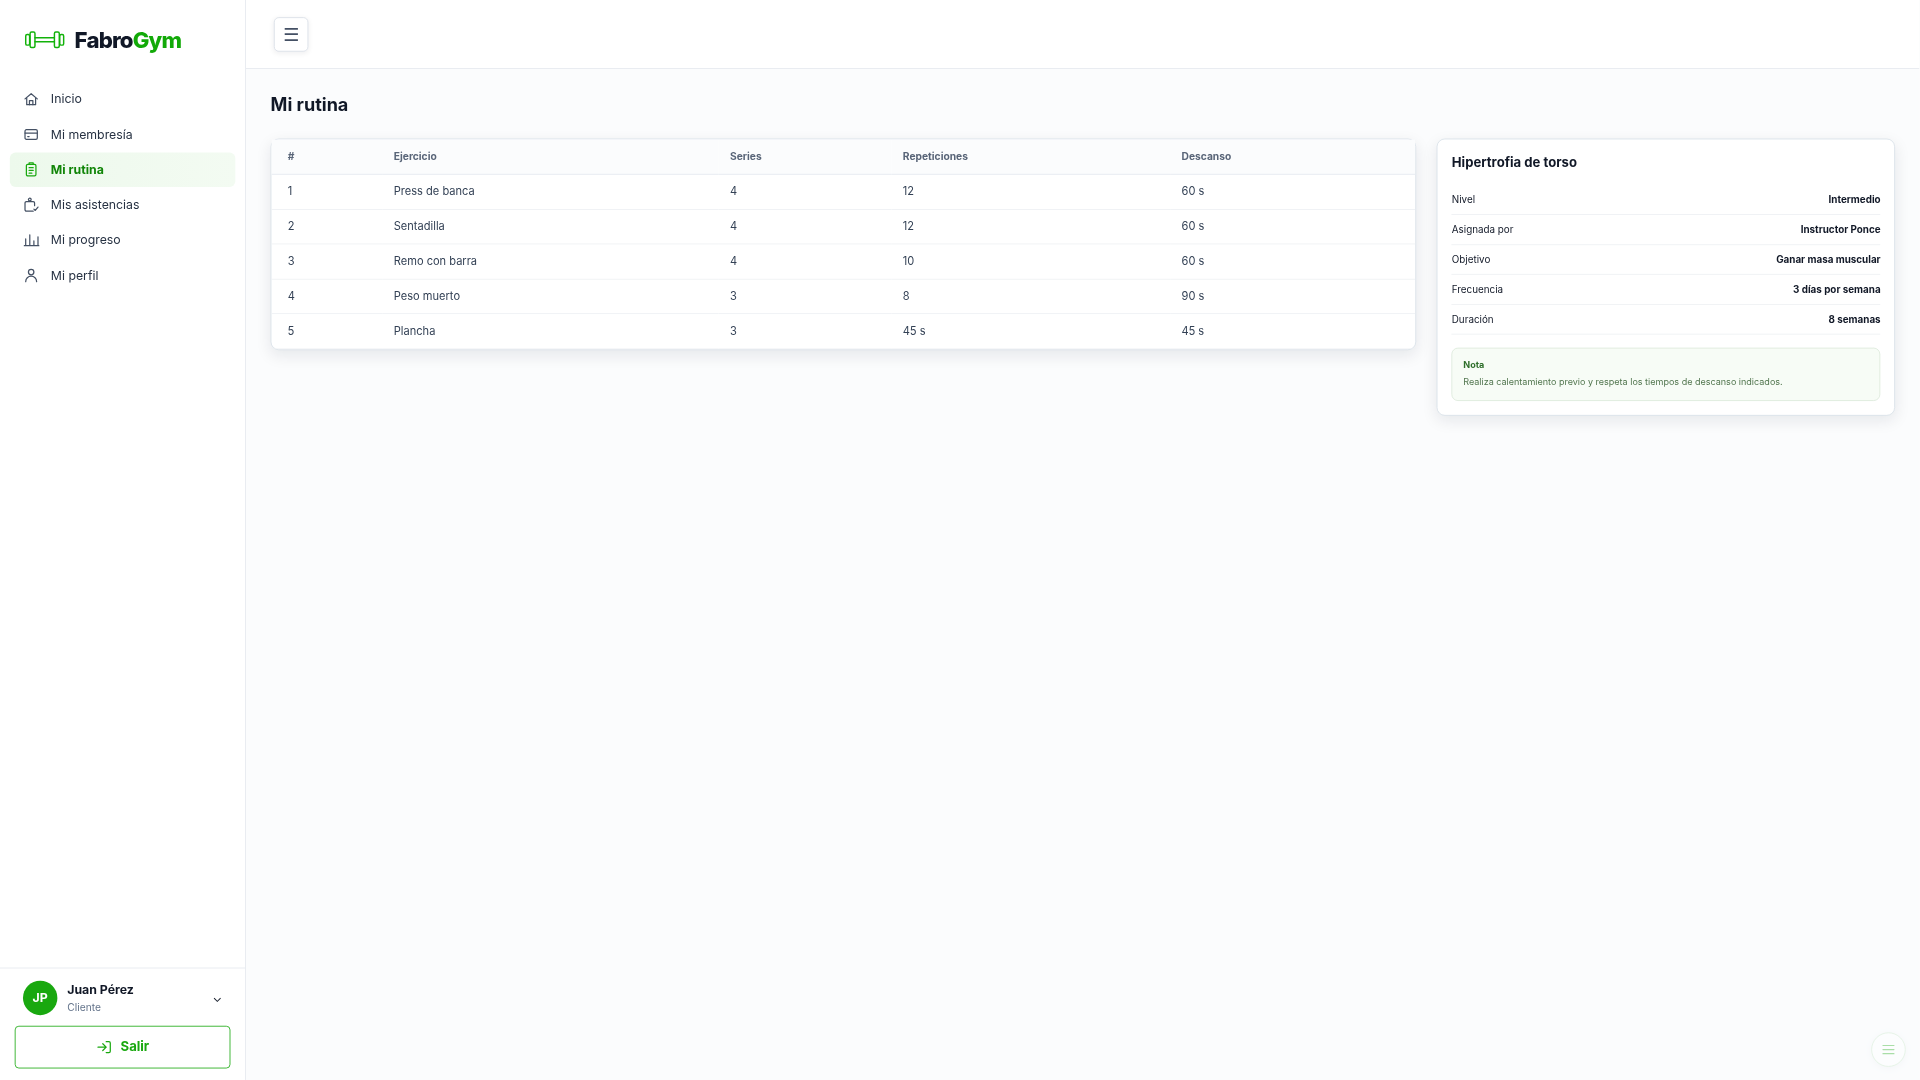
\includegraphics[width=.88\textwidth]{portal_rutina.png}\caption{Portal de consulta de rutina usado como referencia de interfaz para IA-01; no demuestra implementación del modelo.}\end{figure}

\section{Métricas de calidad}

\subsection{Conteos base y criterio de medición}
La auditoría compara la línea base de entrada v1.5.8 (25 RF + 15 RNF = 40 requisitos) con la línea base saneada v2.0 (40 RF + 27 RNF = 67 requisitos). Los valores de referencia corresponden a los umbrales pedagógicos de la guía PE5 \cite{guiaPE5}. Para M6, por definición de la propia guía, el ``antes'' corresponde a la primera re-inspección de PE5 sobre el documento recibido y el ``después'' a la re-inspección posterior al saneamiento, porque esta métrica mide defectos residuales y no funcionalidades pendientes.

\begin{table}[H]
\centering
\caption{Conteos auditables utilizados en las métricas.}
\small
\begin{tabularx}{\textwidth}{|p{4.2cm}|c|c|Y|}
\hline
\textbf{Conteo} & \textbf{Antes} & \textbf{Después} & \textbf{Evidencia de conteo}\\\hline
Requisitos totales & 40 & 67 & ERS v1.5.8 y catálogo v2.0\\\hline
Requisitos con ID, prioridad, fuente y BDD & 34 & 67 & Catálogos RF/RNF y matriz editable\\\hline
Casos de uso identificados / especificados & 19 / 19 & 40 / 40 & Especificaciones textuales y cuatro vistas UML\\\hline
Actores con al menos un RF / actores identificados & 3 / 4 & 5 / 5 & Administrador, Recepción, Instructor, Cliente; luego Superadministrador, Dueño, Recepcionista, Instructor y Cliente\\\hline
Pares de requisitos analizados / conflictos abiertos & 140 / 8 & 140 / 0 & Registro de conflictos y decisiones\\\hline
Requisitos con BDD comprobable & 34 & 67 & Columna Criterio BDD de la matriz\\\hline
RF con cadena adelante completa & 19/25 & 40/40 & Matriz Fuente--RF--CU--Clase--Estado--BDD--CP\\\hline
RF con fuente identificada & 25/25 & 40/40 & Columna Fuente\\\hline
Defectos residuales de redacción detectados en primera re-inspección PE5 & 21 & 0 & Registro de saneamiento y control reproducible en \path{04_Auditoria_Metricas/Registro_Reinspeccion_M6.md}\\\hline
\end{tabularx}
\end{table}

\subsection{Tabla de auditoría antes/después}
\scriptsize
\begin{longtable}{|p{2.2cm}|p{2.5cm}|p{2.5cm}|p{1.9cm}|p{1.5cm}|p{4.1cm}|}
\caption{Auditoría de métricas de calidad del ERS.}\\
\hline\textbf{Métrica} & \textbf{Antes} & \textbf{Después} & \textbf{Referencia} & \textbf{Veredicto} & \textbf{Acción aplicada}\\\hline
\endfirsthead
\hline\textbf{Métrica} & \textbf{Antes} & \textbf{Después} & \textbf{Referencia} & \textbf{Veredicto} & \textbf{Acción aplicada}\\\hline
\endhead
M1a Atributos & $34/40=85,0\%$ & $67/67=100\%$ & $\geq95\%$ & Cumple & Se completaron ID, prioridad, fuente y criterio BDD en los 67 requisitos.\\\hline
M1b CU especificados & $19/19=100\%$ & $40/40=100\%$ & $100\%$ & Cumple & Se especificaron textualmente CU-01 a CU-40 con actor, precondición y escenario observable.\\\hline
M1c Cobertura de actores & $3/4=75,0\%$ & $5/5=100\%$ & $100\%$ & Cumple & Se cerró la ausencia de RF de Cliente y se separaron los roles de administración de la línea base final.\\\hline
M2 Consistencia & $1-8/140=0,943$ & $1-0/140=1,000$ & $\geq0,98$ y 0 abiertos & Cumple & Los ocho conflictos/discrepancias se resolvieron por cambio, delimitación o aclaración documental; las limitaciones de implementación no se cuentan como conflictos.\\\hline
M3 Verificabilidad & $34/40=85,0\%$ & $67/67=100\%$ & $\geq90\%$ & Cumple & Se sustituyeron BDD genéricos de RF por resultados observables y se conservaron umbral, unidad y método en RNF.\\\hline
M4 adelante & $19/25=76,0\%$ & $40/40=100\%$ & $\geq90\%$ & Cumple & Cada RF enlaza CU, clase, proceso/estado, BDD y CP.\\\hline
M4 atrás & $25/25=100\%$ & $40/40=100\%$ & $100\%$ & Cumple & Cada RF conserva una fuente o decisión de diseño explícita.\\\hline
M5 Modificabilidad & $21/5=4,2$ & $12/5=2,4$ & $\leq3,0$ & Cumple & Se mantuvo la separación modular y se revisaron cinco requisitos representativos en la hoja Modificabilidad.\\\hline
M6 Corrección & $21/67=0,313$ & $0/67=0,000$ & $\leq0,05$ & Cumple & Se corrigieron los 21 defectos editoriales registrados y se ejecutó el control reproducible de cierre sobre los 67 requisitos; ver el registro de re-inspección M6 del paquete.\\\hline
\end{longtable}
\normalsize

\subsection{Interpretación y límites}
La evidencia reproducible de M6 conserva el SHA-256 de la ERS inspeccionada, cuenta 40 RF y 27 RNF y verifica 40/40 BDD de RF y 27/27 BDD de RNF. El resultado de M6 no significa que el backend, la restauración, la IA o los walkthroughs no técnicos estén ejecutados. Esas condiciones se registran como \emph{limitaciones de validación o implementación}, no como defectos residuales de redacción del ERS. Del mismo modo, el 100\,\% de M3 expresa verificabilidad documental: cada requisito dispone de un criterio reproducible; no equivale a afirmar que todos los casos de prueba hayan sido ejecutados.


\section{Retrospectiva}
\begin{longtable}{|p{2.2cm}|p{8.2cm}|p{4.2cm}|}\caption{Retrospectiva Start--Stop--Continue.}\\\hline
\textbf{Categoría} & \textbf{Elemento} & \textbf{Responsable}\\\hline\endfirsthead
\hline\textbf{Categoría} & \textbf{Elemento} & \textbf{Responsable}\\\hline\endhead
Start & Vincular cada cambio a un identificador desde su descubrimiento & Alvia Villegas Erick Adalberto \\ \hline
Start & Ejecutar walkthroughs no técnicos antes de cerrar la línea base & Ponce Rivera Mery Helenmey \\ \hline
Start & Mantener criterios BDD y casos de prueba en la misma iteración & Mera Arias Erick Jhair \\ \hline
Stop & Incorporar pantallas sin actualizar alcance y trazabilidad & Mora Duarte Alex José \\ \hline
Stop & Usar etiquetas genéricas como estado o vigencia & Vaca Romero David Octavio \\ \hline
Stop & Confundir prototipo simulado con implementación terminal & Alvia Villegas Erick Adalberto \\ \hline
Continue & Anonimizar evidencias y aplicar minimización de datos & Ponce Rivera Mery Helenmey \\ \hline
Continue & Contrastar RF, mockups y modelos antes de publicar & Mora Duarte Alex José \\ \hline
Continue & Registrar hallazgos, decisiones y limitaciones verificables & Mera Arias Erick Jhair \\ \hline
\end{longtable}

\section{Conclusiones}

\begin{enumerate}
\item La Unidad I permitió delimitar FabroGym como sistema administrativo y operativo, excluyendo salud, biometría y facturación electrónica integrada; esta frontera evitó que los mockups ampliaran silenciosamente el alcance.
\item La Unidad II evidenció que entrevistas, encuesta y documentos organizacionales aportaron fuentes complementarias; la trazabilidad conserva esos orígenes y diferencia evidencia empírica de decisiones internas del equipo.
\item La Unidad III transformó necesidades en 40 RF y 27 RNF verificables, con cinco actores y cuarenta casos de uso conceptuales; la precisión semántica resolvió confusiones sobre estado, vigencia y roles.
\item La Unidad IV mostró que validar no equivale a aprobar todo: tres sesiones técnicas produjeron 18 hallazgos y ocho discrepancias que quedaron cerradas documentalmente; los walkthroughs no técnicos y el backend continúan como limitaciones explícitas, no como conflictos abiertos.
\item La Unidad V integró métricas, trazabilidad e IA responsable: las seis métricas —incluidas las submétricas de completitud y trazabilidad— alcanzan sus umbrales documentales después del saneamiento y los dos componentes de IA conservan control humano, explicación y prohibición de usar datos sensibles.
\end{enumerate}


\section*{Referencias}\addcontentsline{toc}{section}{Referencias}

\begin{thebibliography}{99}
\bibitem{iso29148} ISO/IEC/IEEE, \emph{ISO/IEC/IEEE 29148:2018 Systems and software engineering---Life cycle processes---Requirements engineering}, 2018. [En línea]. Disponible en: \url{https://www.iso.org/standard/72089.html}
\bibitem{iso25010} ISO/IEC, \emph{ISO/IEC 25010:2023 Systems and software engineering---SQuaRE---Product quality model}, 2023. [En línea]. Disponible en: \url{https://www.iso.org/standard/78176.html}
\bibitem{iso15288} ISO/IEC/IEEE, \emph{ISO/IEC/IEEE 15288:2023 Systems and software engineering---System life cycle processes}, 2023. [En línea]. Disponible en: \url{https://www.iso.org/standard/81702.html}
\bibitem{iso12207} ISO/IEC/IEEE, \emph{ISO/IEC/IEEE 12207:2017 Systems and software engineering---Software life cycle processes}, 2017. [En línea]. Disponible en: \url{https://www.iso.org/standard/63712.html}

\bibitem{pohl} K. Pohl, \emph{Requirements Engineering: Fundamentals, Principles, and Techniques}, 2.a ed. Berlin, Alemania: Springer, 2025. ISBN 978-3-662-69204-2.
\bibitem{swebok} IEEE Computer Society, \emph{Guide to the Software Engineering Body of Knowledge, Version 4.0}, 2024. [En línea]. Disponible en: \url{https://www.computer.org/education/bodies-of-knowledge/software-engineering}
\bibitem{ireb} S. Bühne y M. Glinz, \emph{IREB Certified Professional for Requirements Engineering - Foundation Level Syllabus}, versión 3.3.0, International Requirements Engineering Board, 2026. [En línea]. Disponible en: \url{https://cpre.ireb.org/en/downloads-and-resources/downloads}
\bibitem{lopdp} Asamblea Nacional del Ecuador, \emph{Ley Orgánica de Protección de Datos Personales}, Registro Oficial No. 459, Quinto Suplemento, 26 mayo 2021. [En línea]. Disponible en: \url{https://www.asambleanacional.gob.ec/es/multimedios-legislativos/63464-ley-organica-de-proteccion-de-datos}
\bibitem{spdp} Superintendencia de Protección de Datos Personales, \emph{Consultas y criterios sobre bases de legitimación de la LOPDP}, 2025--2026. [En línea]. Disponible en: \url{https://spdp.gob.ec/consultas2025/}
\bibitem{aiact} Parlamento Europeo y Consejo de la Unión Europea, \emph{Reglamento (UE) 2024/1689 por el que se establecen normas armonizadas en materia de inteligencia artificial}, 2024. [En línea]. Disponible en: \url{https://eur-lex.europa.eu/eli/reg/2024/1689/oj/eng}
\bibitem{vogelsang} A. Vogelsang y M. Borg, “Requirements engineering for machine learning: Perspectives from data scientists,” en \emph{2019 IEEE 27th International Requirements Engineering Conference Workshops}, 2019, pp. 245--251, doi: 10.1109/REW.2019.00050.
\bibitem{pmbok} Project Management Institute, \emph{A Guide to the Project Management Body of Knowledge}, 7.a ed. Newtown Square, PA, EE. UU.: PMI, 2021. ISBN 978-1-62825-664-2.
\bibitem{guiaPE5} Universidad Técnica Estatal de Quevedo, \emph{Guía ampliada de práctica experimental PE5: Integración, métricas y defensa del Proyecto Integrador de Ingeniería de Requisitos}, 2026, documento académico suministrado en la asignatura.
\bibitem{sem11} Universidad Técnica Estatal de Quevedo, \emph{Semana 11: Validación de requisitos}, 2026, material de cátedra.
\bibitem{sem13} Universidad Técnica Estatal de Quevedo, \emph{Semana 13: Herramientas CASE y estándares para IR}, 2026, material de cátedra.
\end{thebibliography}


\appendix
\section{Instrumento de auditoría}
La hoja editable \texttt{03\_Matriz\_Trazabilidad/PE5\_Matrices\_FabroGym.xlsx} contiene requisitos, trazabilidad, métricas con fórmulas, backlog, hallazgos, conflictos, modificabilidad, retrospectiva y aportes.

\subsection{Conteos base y criterio de medición}
La auditoría compara la línea base de entrada v1.5.8 (25 RF + 15 RNF = 40 requisitos) con la línea base saneada v2.0 (40 RF + 27 RNF = 67 requisitos). Los valores de referencia corresponden a los umbrales pedagógicos de la guía PE5 \cite{guiaPE5}. Para M6, por definición de la propia guía, el ``antes'' corresponde a la primera re-inspección de PE5 sobre el documento recibido y el ``después'' a la re-inspección posterior al saneamiento, porque esta métrica mide defectos residuales y no funcionalidades pendientes.

\begin{table}[H]
\centering
\caption{Conteos auditables utilizados en las métricas.}
\small
\begin{tabularx}{\textwidth}{|p{4.2cm}|c|c|Y|}
\hline
\textbf{Conteo} & \textbf{Antes} & \textbf{Después} & \textbf{Evidencia de conteo}\\\hline
Requisitos totales & 40 & 67 & ERS v1.5.8 y catálogo v2.0\\\hline
Requisitos con ID, prioridad, fuente y BDD & 34 & 67 & Catálogos RF/RNF y matriz editable\\\hline
Casos de uso identificados / especificados & 19 / 19 & 40 / 40 & Especificaciones textuales y cuatro vistas UML\\\hline
Actores con al menos un RF / actores identificados & 3 / 4 & 5 / 5 & Administrador, Recepción, Instructor, Cliente; luego Superadministrador, Dueño, Recepcionista, Instructor y Cliente\\\hline
Pares de requisitos analizados / conflictos abiertos & 140 / 8 & 140 / 0 & Registro de conflictos y decisiones\\\hline
Requisitos con BDD comprobable & 34 & 67 & Columna Criterio BDD de la matriz\\\hline
RF con cadena adelante completa & 19/25 & 40/40 & Matriz Fuente--RF--CU--Clase--Estado--BDD--CP\\\hline
RF con fuente identificada & 25/25 & 40/40 & Columna Fuente\\\hline
Defectos residuales de redacción detectados en primera re-inspección PE5 & 21 & 0 & Registro de saneamiento y control reproducible en \path{04_Auditoria_Metricas/Registro_Reinspeccion_M6.md}\\\hline
\end{tabularx}
\end{table}

\subsection{Tabla de auditoría antes/después}
\scriptsize
\begin{longtable}{|p{2.2cm}|p{2.5cm}|p{2.5cm}|p{1.9cm}|p{1.5cm}|p{4.1cm}|}
\caption{Auditoría de métricas de calidad del ERS.}\\
\hline\textbf{Métrica} & \textbf{Antes} & \textbf{Después} & \textbf{Referencia} & \textbf{Veredicto} & \textbf{Acción aplicada}\\\hline
\endfirsthead
\hline\textbf{Métrica} & \textbf{Antes} & \textbf{Después} & \textbf{Referencia} & \textbf{Veredicto} & \textbf{Acción aplicada}\\\hline
\endhead
M1a Atributos & $34/40=85,0\%$ & $67/67=100\%$ & $\geq95\%$ & Cumple & Se completaron ID, prioridad, fuente y criterio BDD en los 67 requisitos.\\\hline
M1b CU especificados & $19/19=100\%$ & $40/40=100\%$ & $100\%$ & Cumple & Se especificaron textualmente CU-01 a CU-40 con actor, precondición y escenario observable.\\\hline
M1c Cobertura de actores & $3/4=75,0\%$ & $5/5=100\%$ & $100\%$ & Cumple & Se cerró la ausencia de RF de Cliente y se separaron los roles de administración de la línea base final.\\\hline
M2 Consistencia & $1-8/140=0,943$ & $1-0/140=1,000$ & $\geq0,98$ y 0 abiertos & Cumple & Los ocho conflictos/discrepancias se resolvieron por cambio, delimitación o aclaración documental; las limitaciones de implementación no se cuentan como conflictos.\\\hline
M3 Verificabilidad & $34/40=85,0\%$ & $67/67=100\%$ & $\geq90\%$ & Cumple & Se sustituyeron BDD genéricos de RF por resultados observables y se conservaron umbral, unidad y método en RNF.\\\hline
M4 adelante & $19/25=76,0\%$ & $40/40=100\%$ & $\geq90\%$ & Cumple & Cada RF enlaza CU, clase, proceso/estado, BDD y CP.\\\hline
M4 atrás & $25/25=100\%$ & $40/40=100\%$ & $100\%$ & Cumple & Cada RF conserva una fuente o decisión de diseño explícita.\\\hline
M5 Modificabilidad & $21/5=4,2$ & $12/5=2,4$ & $\leq3,0$ & Cumple & Se mantuvo la separación modular y se revisaron cinco requisitos representativos en la hoja Modificabilidad.\\\hline
M6 Corrección & $21/67=0,313$ & $0/67=0,000$ & $\leq0,05$ & Cumple & Se corrigieron los 21 defectos editoriales registrados y se ejecutó el control reproducible de cierre sobre los 67 requisitos; ver el registro de re-inspección M6 del paquete.\\\hline
\end{longtable}
\normalsize

\subsection{Interpretación y límites}
La evidencia reproducible de M6 conserva el SHA-256 de la ERS inspeccionada, cuenta 40 RF y 27 RNF y verifica 40/40 BDD de RF y 27/27 BDD de RNF. El resultado de M6 no significa que el backend, la restauración, la IA o los walkthroughs no técnicos estén ejecutados. Esas condiciones se registran como \emph{limitaciones de validación o implementación}, no como defectos residuales de redacción del ERS. Del mismo modo, el 100\,\% de M3 expresa verificabilidad documental: cada requisito dispone de un criterio reproducible; no equivale a afirmar que todos los casos de prueba hayan sido ejecutados.


\section{Banco de preguntas de defensa}
\begin{enumerate}
\item ¿Cuál es la frontera de FabroGym y qué se excluye deliberadamente?
\item Muestre un RF e identifique la evidencia concreta que lo originó.
\item ¿Qué diferencia existe entre requisito, historia, caso de uso y prueba?
\item ¿Qué métrica obtuvo el peor resultado antes de la corrección?
\item ¿Por qué V7 no se presenta como MVP terminal?
\item ¿Qué decide IA-01 y qué ocurre si falla?
\item ¿Cómo se controla la equidad de IA-02?
\item ¿Qué limitaciones permanecen abiertas y por qué no se ocultaron?
\end{enumerate}

\section{Product backlog propuesto}

\begin{landscape}\scriptsize
\begin{longtable}{|p{1.6cm}|p{2cm}|p{2.2cm}|p{7.2cm}|p{5.5cm}|p{1.8cm}|}
\caption{Product backlog propuesto y sincronizado con los RF. No se presenta como exportación histórica de una herramienta CASE.}\\
\hline\textbf{Clave} & \textbf{Épica} & \textbf{RF} & \textbf{Historia} & \textbf{Aceptación} & \textbf{Prioridad}\\\hline\endfirsthead
\hline\textbf{Clave} & \textbf{Épica} & \textbf{RF} & \textbf{Historia} & \textbf{Aceptación} & \textbf{Prioridad}\\\hline\endhead
PFC-001 & Acceso y seguridad & RF-AUT-01 & Como Personal autorizado, quiero autenticar usuario para proteger las operaciones y conservar trazabilidad. & Dado un usuario con credenciales válidas, cuando inicie sesión, entonces el sistema deberá autenticarlo y habilitar únicamente las opciones permitidas para su rol; cuando cierre sesión, deberá invalidar la sesión activa. & Must \\ \hline
PFC-002 & Acceso y seguridad & RF-AUT-02 & Como Administrador, quiero aplicar permisos por rol para proteger las operaciones y conservar trazabilidad. & Dado un usuario autenticado con un rol definido, cuando intente ejecutar una operación, entonces el sistema deberá permitirla solo si el permiso está asignado a ese rol y deberá denegarla en caso contrario. & Must \\ \hline
PFC-003 & Acceso y seguridad & RF-AUT-03 & Como Administrador, quiero auditar cambios criticos para proteger las operaciones y conservar trazabilidad. & Dado un cambio crítico confirmado, cuando el sistema lo registre, entonces deberá conservar en auditoría el actor, fecha, acción, valor anterior y valor nuevo asociados al cambio. & Should \\ \hline
PFC-004 & Clientes & RF-CLI-01 & Como Recepcionista, quiero registrar cliente minimo para mantener registros únicos y consultables. & Dado un formulario con código interno, nombre de uso y al menos un medio de contacto válido, cuando Recepción confirme el registro, entonces el sistema deberá crear un único cliente y no deberá solicitar datos de salud, biometría, dirección domiciliaria ni imagen corporal. & Must \\ \hline
PFC-005 & Clientes & RF-CLI-02 & Como Recepcionista, quiero buscar y consultar cliente para mantener registros únicos y consultables. & Dado un criterio de búsqueda válido, cuando Recepción consulte un cliente, entonces el sistema deberá devolver las coincidencias y mostrar únicamente membresía, último pago, asistencia y novedades autorizadas por el rol. & Must \\ \hline
PFC-006 & Clientes & RF-CLI-03 & Como Recepcionista, quiero actualizar o reactivar sin duplicar para mantener registros únicos y consultables. & Dado que existe un cliente coincidente por código o contacto, cuando Recepción intente registrar o reactivar el perfil, entonces el sistema deberá advertir la coincidencia y permitir actualizar o reactivar el registro existente sin crear un duplicado. & Must \\ \hline
PFC-007 & Membresías & RF-MEM-01 & Como Administrador, quiero configurar planes y promociones para controlar la vigencia del servicio. & Dado un usuario autorizado y los datos obligatorios de un plan o promoción, cuando guarde la configuración, entonces el sistema deberá conservar nombre, duración, precio, vigencia y estado y deberá mostrar el registro actualizado. & Must \\ \hline
PFC-008 & Membresías & RF-MEM-02 & Como Recepcionista, quiero activar o renovar membresia para controlar la vigencia del servicio. & Dado un plan vigente y un pago confirmado, cuando Recepción active o renueve la membresía, entonces el sistema deberá calcular y guardar las fechas de inicio y vencimiento según la duración del plan. & Must \\ \hline
PFC-009 & Membresías & RF-MEM-03 & Como Personal autorizado, quiero consultar vigencia para controlar la vigencia del servicio. & Dado un cliente con membresía registrada, cuando un usuario autorizado consulte su vigencia, entonces el sistema deberá mostrar estado, plan, fecha de inicio y fecha de vencimiento de la membresía seleccionada. & Must \\ \hline
PFC-010 & Membresías & RF-MEM-04 & Como Recepcionista, quiero alertar vencimientos para controlar la vigencia del servicio. & Dado que existen membresías próximas a vencer o vencidas, cuando se ejecute la consulta diaria, entonces el sistema deberá separar las que vencen dentro de tres días de las ya vencidas y no deberá enviar mensajes externos de forma automática. & Must \\ \hline
PFC-011 & Pagos & RF-PAG-01 & Como Recepcionista, quiero registrar pago y comprobante para mantener pagos verificables. & Dado un pago con monto, concepto, medio, referencia y fecha válidos, cuando Recepción confirme el registro, entonces el sistema deberá guardar el pago y generar un comprobante interno vinculado al cliente. & Must \\ \hline
PFC-012 & Pagos & RF-PAG-02 & Como Administrador, quiero resolver pago pendiente para mantener pagos verificables. & Dado un pago con estado pendiente, cuando un Administrador lo confirme, rechace o corrija, entonces el sistema deberá actualizar el estado y conservar el motivo y la evidencia de auditoría de la decisión. & Should \\ \hline
PFC-013 & Asistencias & RF-ASI-01 & Como Recepcionista, quiero registrar asistencia para registrar el uso del gimnasio. & Dado un cliente identificado, cuando Recepción registre la asistencia por QR, entonces el sistema deberá guardar fecha, hora y método QR; si se utiliza contingencia manual, deberá exigir responsable y motivo. & Must \\ \hline
PFC-014 & Asistencias & RF-ASI-02 & Como Personal autorizado, quiero consultar asistencia para registrar el uso del gimnasio. & Dado un filtro por cliente, fecha o turno, cuando un usuario autorizado consulte asistencias, entonces el sistema deberá mostrar únicamente los registros que cumplan el filtro y los conteos correspondientes. & Must \\ \hline
PFC-015 & Inventario & RF-INV-01 & Como Administrador, quiero administrar productos para mantener existencias consistentes. & Dado un producto con código, nombre, precio, unidad, stock mínimo y estado válidos, cuando el Administrador confirme el registro, entonces el sistema deberá guardar el producto y permitir su consulta posterior. & Must \\ \hline
PFC-016 & Inventario & RF-INV-02 & Como Personal autorizado, quiero registrar movimientos de stock para mantener existencias consistentes. & Dado un producto existente y un movimiento válido, cuando un usuario autorizado registre una entrada o ajuste, entonces el sistema deberá actualizar el saldo y conservar cantidad, motivo, responsable y saldo resultante. & Must \\ \hline
PFC-017 & Ventas & RF-VEN-01 & Como Recepcionista, quiero registrar venta para integrar venta, pago y stock. & Dado que todos los ítems de una venta tienen stock suficiente, cuando Recepción confirme la venta, entonces el sistema deberá registrar la venta y descontar las existencias en una única transacción; si falla una operación, no deberá aplicar cambios parciales. & Must \\ \hline
PFC-018 & Inventario & RF-INV-03 & Como Administrador, quiero alertar stock y rotacion para mantener existencias consistentes. & Dado un período de consulta, cuando el Administrador solicite el control de stock, entonces el sistema deberá listar los productos con stock igual o inferior al mínimo y resumir entradas, salidas y ventas del período. & Should \\ \hline
PFC-019 & Caja & RF-CAJ-01 & Como Recepcionista, quiero cerrar turno y conciliar caja para cerrar el turno con diferencias visibles. & Dado un turno con pagos y ventas registrados, cuando Recepción ejecute el cierre, entonces el sistema deberá totalizar por medio de pago, comparar contra los valores declarados y registrar cualquier diferencia junto con la entrega del turno. & Must \\ \hline
PFC-020 & Novedades & RF-NOV-01 & Como Personal autorizado, quiero gestionar novedades internas para dar seguimiento a incidencias. & Dado un usuario autorizado y una novedad con categoría, detalle, responsable y vencimiento, cuando la registre, entonces el sistema deberá crearla con un estado válido y conservar los cambios posteriores de estado. & Must \\ \hline
PFC-021 & Instructores & RF-INS-01 & Como Administrador, quiero gestionar horario y disponibilidad de instructor para coordinar la disponibilidad del personal. & Dado un instructor registrado, cuando el Administrador actualice su operación, entonces el sistema deberá guardar turnos, capacidad, disponibilidad y novedades operativas sin solicitar datos de salud. & Should \\ \hline
PFC-022 & Rutinas & RF-RUT-01 & Como Instructor, quiero crear y asignar rutina para personalizar y consultar el entrenamiento. & Dado un cliente autorizado y un catálogo de ejercicios disponible, cuando el Instructor cree una rutina, entonces el sistema deberá guardar objetivo operativo, ejercicios, series, repeticiones, descanso y días, y deberá asignarla al cliente seleccionado. & Must \\ \hline
PFC-023 & Rutinas & RF-RUT-02 & Como Instructor, quiero versionar y ajustar rutina para personalizar y consultar el entrenamiento. & Dado una rutina existente, cuando el Instructor modifique ejercicios o parámetros y confirme el cambio, entonces el sistema deberá crear una nueva versión y mantener las versiones anteriores en solo lectura. & Must \\ \hline
PFC-024 & Rutinas & RF-RUT-03 & Como Instructor, quiero registrar seguimiento operativo para personalizar y consultar el entrenamiento. & Dado una rutina activa, cuando el Instructor registre seguimiento, entonces el sistema deberá guardar fecha, cumplimiento, repeticiones y observación operativa y deberá rechazar campos destinados a diagnósticos, lesiones, peso o medidas corporales reales. & Should \\ \hline
PFC-025 & Reportes & RF-REP-01 & Como Administrador, quiero consultar panel y reportes para tomar decisiones con información reproducible. & Dado un período y filtros válidos, cuando el Administrador consulte el panel o reporte, entonces el sistema deberá calcular los indicadores con datos almacenados, mostrar los resultados filtrados y permitir exportarlos a CSV. & Should \\ \hline
PFC-026 & Membresías & RF-MEM-05 & Como Cliente, quiero consultar mi membresía para controlar la vigencia del servicio. & Dado un Cliente autenticado, cuando consulte su membresía, entonces el sistema deberá mostrar únicamente el estado, plan y vigencia de su propia membresía y no deberá habilitar edición. & Must \\ \hline
PFC-027 & Pagos & RF-PAG-03 & Como Cliente, quiero consultar mis pagos para mantener pagos verificables. & Dado un Cliente autenticado, cuando consulte sus pagos, entonces el sistema deberá mostrar únicamente sus registros de pago y el estado de cada uno en modo de solo lectura. & Must \\ \hline
PFC-028 & Rutinas & RF-RUT-04 & Como Cliente, quiero consultar mi rutina e historial para personalizar y consultar el entrenamiento. & Dado un Cliente autenticado con una rutina asignada, cuando consulte su rutina, entonces el sistema deberá mostrar la versión activa, las versiones históricas y el seguimiento autorizado sin permitir modificar la rutina vigente. & Must \\ \hline
PFC-029 & Inventario & RF-INV-04 & Como Dueño, quiero gestionar categorías de productos para mantener existencias consistentes. & Dado un usuario autorizado, cuando registre, edite o desactive una categoría, entonces el sistema deberá guardar el cambio y reflejar el estado actualizado en las consultas de categorías. & Should \\ \hline
PFC-030 & Inventario & RF-INV-05 & Como Dueño, quiero gestionar proveedores para mantener existencias consistentes. & Dado un usuario autorizado, cuando registre, edite o desactive un proveedor, entonces el sistema deberá guardar el cambio y reflejar el estado actualizado en las consultas de proveedores. & Should \\ \hline
PFC-031 & Configuración & RF-CFG-01 & Como Dueño, quiero configurar tratamiento de iva para adaptar reglas sin modificar código. & Dado un porcentaje de IVA válido y la configuración tributaria de un producto, cuando el Dueño confirme el cambio, entonces el sistema deberá aplicar la nueva configuración a operaciones posteriores y conservar el valor anterior, el nuevo valor, el actor y la fecha. & Must \\ \hline
PFC-032 & Continuidad & RF-BCK-01 & Como Superadministrador, quiero generar respaldo para recuperar la operación ante fallos. & Dado un Superadministrador autenticado, cuando solicite un respaldo, entonces el sistema deberá iniciar el proceso cifrado, asignar un identificador y mostrar el estado y la fecha de finalización cuando concluya. & Should \\ \hline
PFC-033 & Continuidad & RF-BCK-02 & Como Superadministrador, quiero restaurar respaldo para recuperar la operación ante fallos. & Dado un respaldo íntegro seleccionado, cuando el Superadministrador confirme explícitamente la restauración, entonces el sistema deberá verificar su integridad, ejecutar la restauración y registrar la operación en auditoría; si la verificación falla, no deberá restaurar. & Should \\ \hline
PFC-034 & Configuración & RF-CFG-02 & Como Dueño, quiero configurar horario de atención para adaptar reglas sin modificar código. & Dado un Dueño autenticado y una configuración válida de días y horas, cuando guarde el horario, entonces el sistema deberá actualizarlo y mostrar al Cliente únicamente el horario vigente. & Could \\ \hline
PFC-035 & Inteligencia artificial & RF-IA-RUT-01 & Como Cliente/Instructor, quiero generar recomendación de rutina para apoyar decisiones sin sustituir al usuario. & Dado un objetivo operativo, disponibilidad semanal, historial no sensible y catálogo autorizado, cuando se solicite una recomendación, entonces el componente deberá devolver como máximo tres alternativas ordenadas de rutina y una explicación de los factores utilizados. & Must \\ \hline
PFC-036 & Inteligencia artificial & RF-IA-RUT-02 & Como Cliente, quiero aceptar, rechazar o solicitar alternativa para apoyar decisiones sin sustituir al usuario. & Dado que el Cliente visualiza una recomendación de rutina, cuando seleccione aceptar, rechazar o solicitar alternativa, entonces el sistema deberá registrar la decisión y no deberá activar automáticamente la recomendación. & Must \\ \hline
PFC-037 & Inteligencia artificial & RF-IA-RUT-03 & Como Instructor, quiero revisar recomendación de rutina para apoyar decisiones sin sustituir al usuario. & Dado una recomendación aceptada por el Cliente, cuando el Instructor la revise, entonces el sistema deberá permitir aprobarla o rechazarla con motivo; únicamente una aprobación explícita podrá habilitar su activación. & Must \\ \hline
PFC-038 & Inteligencia artificial & RF-IA-ABA-01 & Como Dueño, quiero calcular riesgo de inactividad para apoyar decisiones sin sustituir al usuario. & Dado el historial de asistencia, vigencia de membresía y frecuencia histórica de un cliente, cuando se ejecute el cálculo semanal, entonces el componente deberá asignar un nivel bajo, medio o alto y registrar la fecha del cálculo. & Should \\ \hline
PFC-039 & Inteligencia artificial & RF-IA-ABA-02 & Como Dueño/Recepcionista, quiero mostrar alertas de riesgo para apoyar decisiones sin sustituir al usuario. & Dado que existen clientes clasificados con riesgo medio o alto, cuando Dueño o Recepcionista consulte las alertas, entonces el sistema deberá mostrar el nivel, la fecha y los principales factores de cada alerta sin ejecutar acciones automáticas. & Should \\ \hline
PFC-040 & Inteligencia artificial & RF-IA-ABA-03 & Como Recepcionista, quiero registrar seguimiento de alerta para apoyar decisiones sin sustituir al usuario. & Dado una alerta de riesgo visible, cuando Recepción registre contacto, aplazamiento o descarte, entonces el sistema deberá guardar la acción, responsable, fecha y observación para auditoría. & Should \\ \hline
\end{longtable}\end{landscape}


\section{Aportes individuales de la actividad PE5}
\begin{longtable}{|p{4cm}|p{6.2cm}|p{4.3cm}|}\hline
\textbf{Integrante} & \textbf{Aporte asignado en la actividad} & \textbf{Evidencia verificable en Git}\\\hline
Alvia Villegas Erick Adalberto & Integración metodológica, control de alcance y consolidación del informe & \texttt{01\_Informe\_Final/}; \texttt{05\_Gestion/Backlog\_Propuesto.md} \\ \hline
Mera Arias Erick Jhair & Auditoría de métricas, trazabilidad end-to-end y control de cobertura & \texttt{03\_Matriz\_Trazabilidad/}; \texttt{04\_Auditoria\_Metricas/}; \texttt{\_generados/metricas.tex}; \texttt{\_generados/trazabilidad.tex} \\ \hline
Mora Duarte Alex José & Modelos UML, casos de uso y consistencia entre modelos y ERS & \texttt{diagramas\_fuente/}; \texttt{assets/}; \texttt{\_generados/casos\_uso.tex} \\ \hline
Ponce Rivera Mery Helenmey & Validación, consolidación de hallazgos y re-inspección del ERS & \texttt{05\_Gestion/Validacion/}; \texttt{\_generados/validacion.tex} \\ \hline
Vaca Romero David Octavio & Gestión documental, backlog, retrospectiva y reproducibilidad & \texttt{README.md}; \texttt{05\_Gestion/}; \texttt{CHANGELOG.md} \\ \hline
\end{longtable}
La presente PE5 corresponde al PFC FabroGym del Equipo F. La contribución individual se verifica mediante el historial real del repositorio de la actividad, los archivos modificados y las fechas de los commits. La distribución indicada identifica responsabilidades de cierre y no atribuye commits que todavía no existan; antes de congelar la línea base, cada integrante debe comprobar que su declaración coincide con el historial Git.

\section{Declaración de uso de IA}
De conformidad con la Guía Ampliada de la PE5, el uso de inteligencia artificial se declara \textbf{por sección}, identificando la herramienta empleada, el tipo de asistencia y el método utilizado para validar el contenido. Se utilizó \textbf{ChatGPT (OpenAI)} como herramienta de apoyo. La IA no se utilizó como fuente de evidencia empírica ni para atribuir entrevistas, actas, implementaciones, resultados de pruebas, métricas o commits inexistentes. En las secciones evaluativas, la asistencia se limitó a apoyo de redacción, organización, revisión de consistencia y generación de código o tablas; las afirmaciones técnicas se contrastaron con los artefactos disponibles; antes de la entrega, el Equipo F debe revisar, comprender y asumir la versión final del contenido.

{\footnotesize\begin{longtable}{|p{2.4cm}|p{2.0cm}|p{3.6cm}|p{5.9cm}|}
\caption{Declaración verificable del uso de IA por sección del informe.}\\\hline
\textbf{Sección} & \textbf{Herramienta} & \textbf{Tipo de asistencia} & \textbf{Método de validación}\\\hline
\endfirsthead
\hline\textbf{Sección} & \textbf{Herramienta} & \textbf{Tipo de asistencia} & \textbf{Método de validación}\\\hline
\endhead
Carátula y preliminares & ChatGPT & Revisión de formato y consistencia de datos. & Contraste de nombres, asignatura, periodo, versión y URL con los datos de la actividad y el repositorio de la actividad PE5.\\\hline
Resumen y Abstract & ChatGPT & Redacción asistida y traducción del resumen al inglés. & Verificación de cifras, alcance y limitaciones contra el cuerpo del informe, la ERS final y la matriz; revisión final del sentido técnico exigida al equipo antes de entregar.\\\hline
1. Introducción & ChatGPT & Redacción asistida y revisión de estilo. & Contraste del contexto, alcance y conformación del Equipo F con los artefactos de FabroGym y las condiciones de la actividad PE5.\\\hline
2. Metodología de IR & ChatGPT & Estructuración, redacción asistida y revisión de consistencia. & Comprobación contra ISO/IEC/IEEE 29148:2018, SWEBOK, Pohl, materiales de las semanas 11 y 13 y las técnicas realmente documentadas en el paquete.\\\hline
3. ERS/SRS final & ChatGPT & Revisión editorial, saneamiento lingüístico, reformulación de criterios BDD y apoyo con código LaTeX. & Contraste de identificadores, fuentes, prioridades, BDD y casos de prueba con la ERS de entrada, la ERS v2.0.3 y la matriz de trazabilidad; no se añadieron evidencias de campo inexistentes.\\\hline
4. Modelos UML & ChatGPT & Organización de vistas y apoyo en código reproducible LaTeX/Graphviz para DFD, estados y secuencias. & Verificación de actores, CU, procesos P-01--P-15, estados e identificadores contra la ERS y la matriz; revisión visual de los PDF generados; los modelos no se presentan como evidencia de backend.\\\hline
5. Validación & ChatGPT & Síntesis, redacción asistida y revisión de consistencia. & Contraste con el informe y la matriz consolidados de validación disponibles; la evidencia identificable se resguarda fuera del repositorio público. Los walkthroughs no técnicos se mantienen expresamente como no ejecutados y no se contabilizan como evidencia.\\\hline
6. Gestión y trazabilidad & ChatGPT & Estructuración de tablas, revisión de enlaces y apoyo para fórmulas/hojas de cálculo. & Revisión fila por fila de la cadena Fuente--RF--CU--Clase--DFD--Estado--BDD--CP y contraste con el backlog y la ERS; comprobación de fórmulas en el archivo Excel.\\\hline
7. Requisitos de IA & ChatGPT & Generación de propuestas, redacción asistida y revisión de requisitos medibles. & Validación de pertinencia con el dominio FabroGym, trazabilidad con RF existentes y contraste normativo con la LOPDP y el Reglamento (UE) 2024/1689. Los componentes se declaran como especificados, no implementados.\\\hline
8. Métricas de calidad & ChatGPT & Apoyo en aritmética, tablas, fórmulas y script de re-inspección documental. & Recuento sobre la misma ERS entregada, contraste con Excel y ejecución reproducible de M6 sobre 40 RF + 27 RNF con registro del SHA-256 de la ERS.\\\hline
9. Retrospectiva & ChatGPT & Organización y redacción asistida del formato Start--Stop--Continue. & Contraste de acciones y responsables con las limitaciones y decisiones documentadas; el equipo debe confirmar su pertinencia antes de entregar.\\\hline
10. Conclusiones & ChatGPT & Apoyo de síntesis y mejora de redacción. & Cada conclusión se contrastó con los resultados de las Unidades I--V y con los artefactos citados; el equipo debe revisar, comprender y asumir su formulación final antes de entregar.\\\hline
Referencias & ChatGPT & Normalización de formato IEEE y revisión bibliográfica. & Verificación de normas en sitios oficiales y de DOI/ISBN cuando corresponde; eliminación de referencias no utilizadas o no verificables.\\\hline
Anexos & ChatGPT & Generación de tablas, revisión de formato y organización documental. & Contraste con archivos fuente del paquete, matrices editables, registros de validación y manifiesto SHA-256; los anexos no sustituyen evidencia ausente.\\\hline
\end{longtable}

\textbf{Criterio de responsabilidad.} El equipo reconoce que declarar el uso de IA no sustituye la autoría ni la comprensión exigidas en la defensa. Por ello, cualquier afirmación, decisión de ingeniería, resultado de métrica o conclusión incluida en la entrega debe poder ser explicada y respaldada mediante la ERS, la matriz, los modelos o los anexos correspondientes.

\end{document}
